%%%%%%%%%%%%%%%%%%%%%%%%%%%%%%%%%%%%%%%%%%%%%%%%%%%%%%%%%%%%%%%%%%%%%%%%%%
%%%%%%%%%%%%%%%%%%%%%%%%%%%%%%%%%%%%%%%%%%%%%%%%%%%%%%%%%%%%%%%%%%%%%%%%%%
\clearpage{}
\section{Determination of signal yield from a fit to the \texorpdfstring{$m_{jj}$}{dijet invariant mass} distribution}
\label{sec:mjj_fit}
We extract the diboson signal yield from an unbinned maximum
likelihood fit to the dijet invariant mass distribution in the data.
Table~\ref{tab:mjj_shapes_and_normalization} shows how the shape of
each component is determined, and what constraints are applied to fit
for the normalization; while the fit output is summarized in
Table~\ref{table:FitTotalsAndComparisons}.  The main sources of
systematics error are the uncertainties in the factorization and
renormalization scales ($q^2$) and the matrix element -- parton shower
matching scale in the the leading-order W+jets Monte Carlo, as well as
the jet energy scale (JES) uncertainty.
%%%%%%%%%%%%%%%
\begin{table}[!htbp]
  \begin{center}
 \caption{Determination of the $m_{jj}$ shape and normalization. External constraints are assumed Gaussian.}  
 \label{tab:mjj_shapes_and_normalization} 
 \begin{tabular} {l  c  l}
   \hline \hline
   Process                &    Shape     & External constraint on normalization\\ \hline
   W plus jets            &    MC/data   & Constrained: (NLO) 31314 pb $\pm$ 5\%~\cite{MCFM} \\
   Diboson                &    MC        & Unconstrained \\ 
   \ttbar\                &    MC        & Constrained: (NLO) 163 pb $\pm$ 7\% ~\cite{Kidonakis:2010dk}\\ 
   Single top             &    MC        & Constrained: (NNLO)~\cite{Kidonakis:2010tc,Kidonakis:2011wy,Kidonakis:2010ux} $\pm$ 5\%\\
   Drell-Yan plus jets    &    MC        & Constrained: (NLO, $m_{ll}>50$~GeV) 3048 pb  $\pm$  4.3\%~\cite{MCFM} \\
   Multijet               &    data      & Constrained: \MET fit in data $\pm$  50\% (100\%) for electron (muon) \\\hline \hline
 \end{tabular}
\end{center}
\end{table}
%%%%%%%%%%%%%%%%%%%%%%%%%%%%%%%%%%%%%%%%%%%%%%%%%%%%%%%%%%%%
%%%%%%%%%%%%%%%%%%%%%%%%%%%%%%%%%%%%%%%%%%%%%%%%%%%%%%%%%%%%%%%
%%%\begin{table}[!htbp]
%%%  \begin{center}
%%% \caption{Event yields determined from a likelihood fit
%%% to the data. The total uncertainty takes into
%%% account the correlations among individual components.}
%%% \label{tab:mjj_shapes_and_normalization}
%%% \begin{tabular} {l  c  c c c }
%%%   \hline \hline
%%%   Process             &    \multicolumn{2}{c}{Muon channel} & \multicolumn{2}{c}{Electron channel} \\  
%%%\hline
%%%                       &    2 jets              &  3 jets              & 2 jets             &  3 jets\\  
%%%\hline
%%%   W+jets              &    53231  $\pm$  466   &  12551 $\pm$  331    &  30075 $\pm$ 115   &  8725 $\pm$  273\\
%%%   Dibosons            &    1087 $\pm$  98      &  339 $\pm$  49       &  642 $\pm$  61     &  173 $\pm$  17\\
%%%   $t\bar{t}$          &    3973  $\pm$  238    &  7738 $\pm$  330     &  2313 $\pm$ 143    &  3939 $\pm$  216\\
%%%   Single top          &    1545  $\pm$  76     &  873 $\pm$  43       &  858 $\pm$  43     &  489 $\pm$  24\\
%%%   Drell-Yan+jets      &    1362 $\pm$  58      &  417 $\pm$  18       &  993 $\pm$  43     &  341 $\pm$  15\\
%%%   Multijet            &    84 $\pm$  256       &  0 $\pm$ 90          &  4040 $\pm$ 1170   &  334 $\pm$  160\\
%%%\hline
%%%   Total from fit      &    61281 $\pm$ 290     &  21918 $\pm$ 183     &  38923 $\pm$ 227   &  14000 $\pm$ 141\\
%%%   Data                &    61153               &  22030               &  38973             &  14145 \\
%%%\hline
%%%\multicolumn{5}{c}{in region $(123\,\text{GeV} < m_{jj} < 186\,\text{GeV})$} \\
%%%\hline
%%%  Total from fit & 12921 $\pm$ 118 & 7021 $\pm$ 91 & 7909 $\pm$ 92 & 4297 $\pm$ 70\\
%%%  Data & 12761 & 7111 & 8023 & 4438 \\
%%%\hline \hline
%%% \end{tabular}
%%%\end{center}
%%%\end{table}
%%%%%%%%%%%%%%%%%%%%%%%%%%%%%%%%%%%%%%%%%%%%%%%%%%%%%%%%%%%%%%%
\subsection{Fit results}
\label{sec:mjj_2jetfit}
The results of the fit for the 2-jet sample are shown 
in Figs.~\ref{fig:mjj_2jet_mu} and~\ref{fig:mjj_2jet_el}. 
A clear peak from the Standard Model electroweak diboson 
WW/WZ production can be seen. 
The mean mass, resolution and yield for the diboson events are 
consistent with the Standard Model predictions computed up to 
the next-to-leading order (NLO) in perturbation theory.
These consistency checks give us confidence in the analysis procedures.
The fit results are tabulated below.
%%%%%%%%%%%%%%%%%%%%

\underline{Muons, no b-tag:}
{\tiny
\input{log_Diboson_Muon.log}
}

\underline{Muons, b-tag:}
{\tiny
\input{log_Diboson_Muon_btag.log}
}

\underline{Electrons, no b-tag:}
{\tiny
\input{log_Diboson_Electron.log}
}

\underline{Electrons, b-tag:}
{\tiny
\input{log_Diboson_Electron_btag.log}
}
%%%%%%%%%%%%%%%%%%%%
%%%%%%%%%%%%%%%%%%%%
%%%%%%%%%%%%%%%%%%%%
%%%%%%%%%%%%%%%%%%%%
\begin{figure}[h!]
  {\centering
    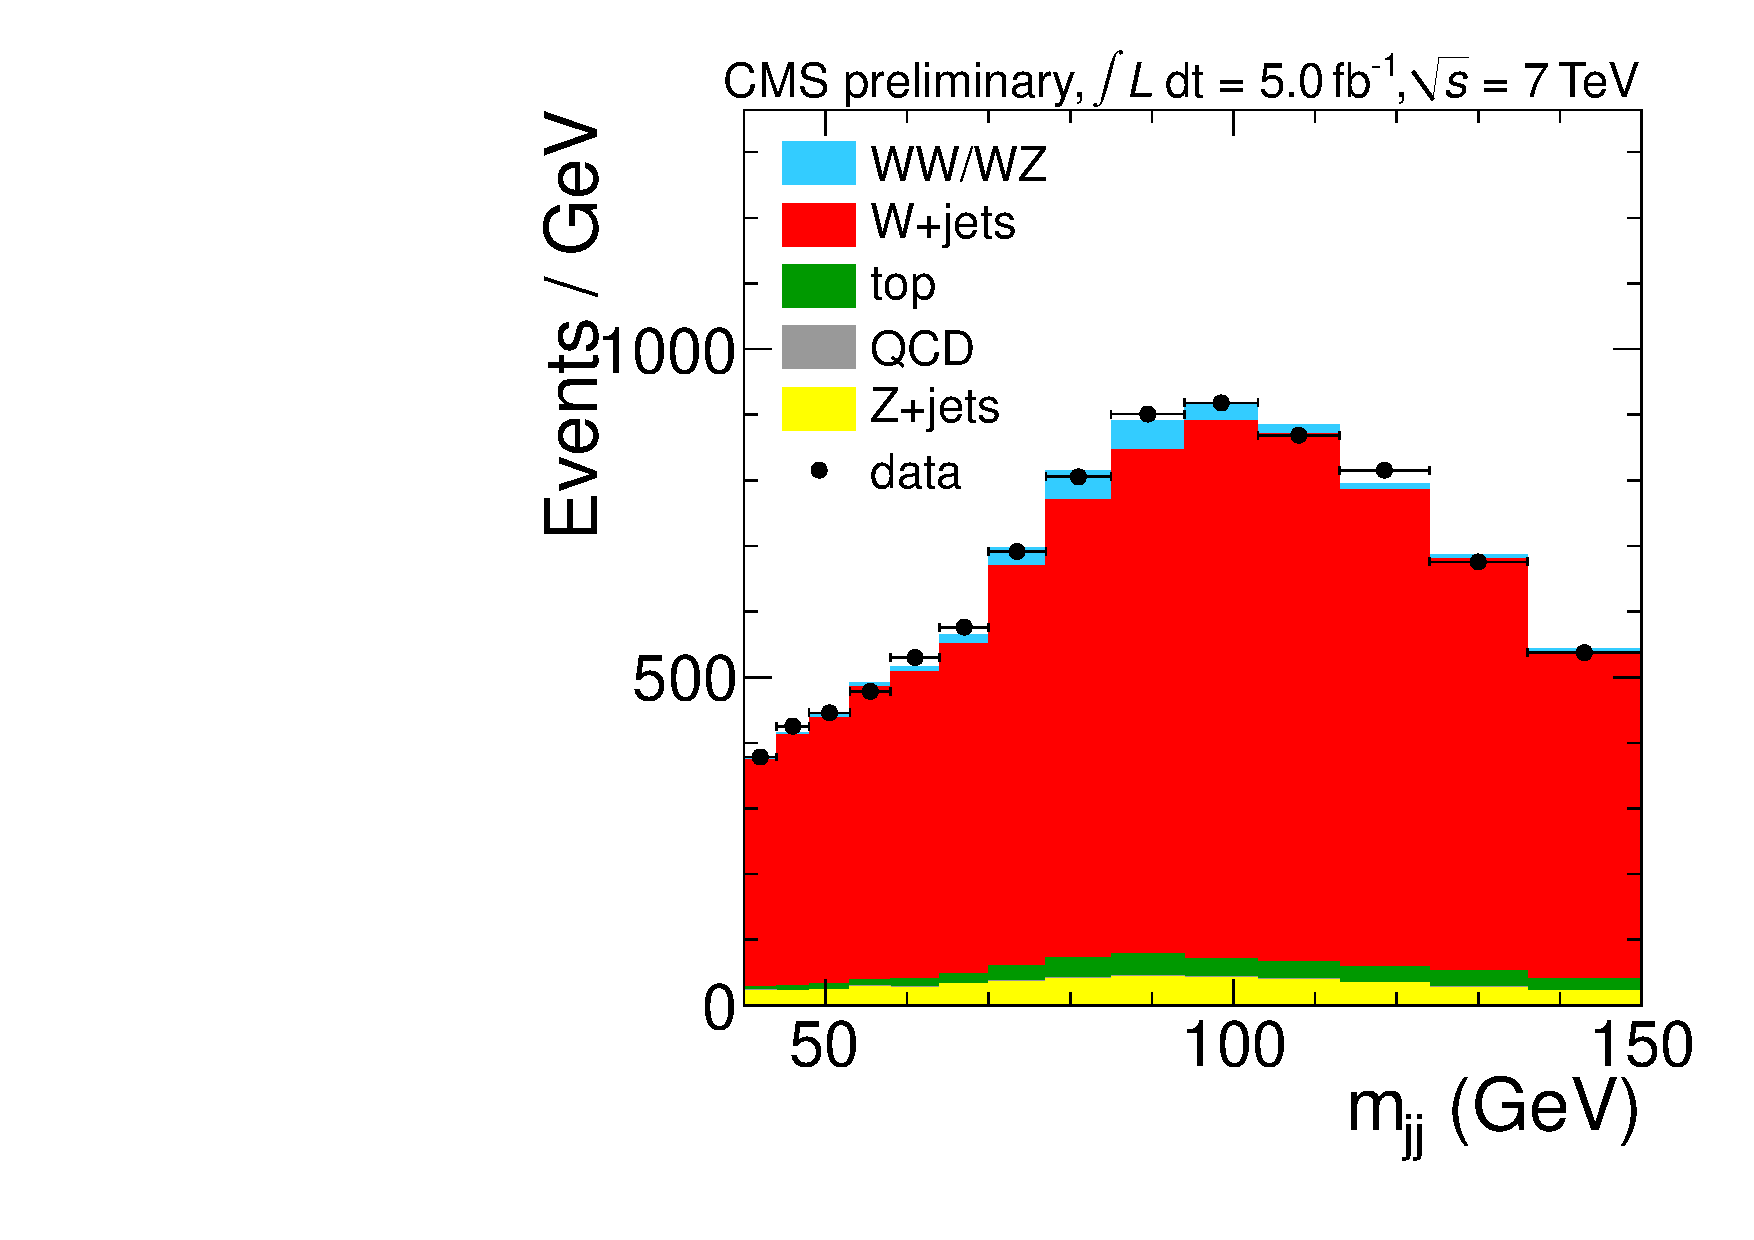
\includegraphics[width=0.49\textwidth]{figs/mjjfit_2jetsample/Wjj_Diboson_Muon_2jets_Stacked.pdf}
    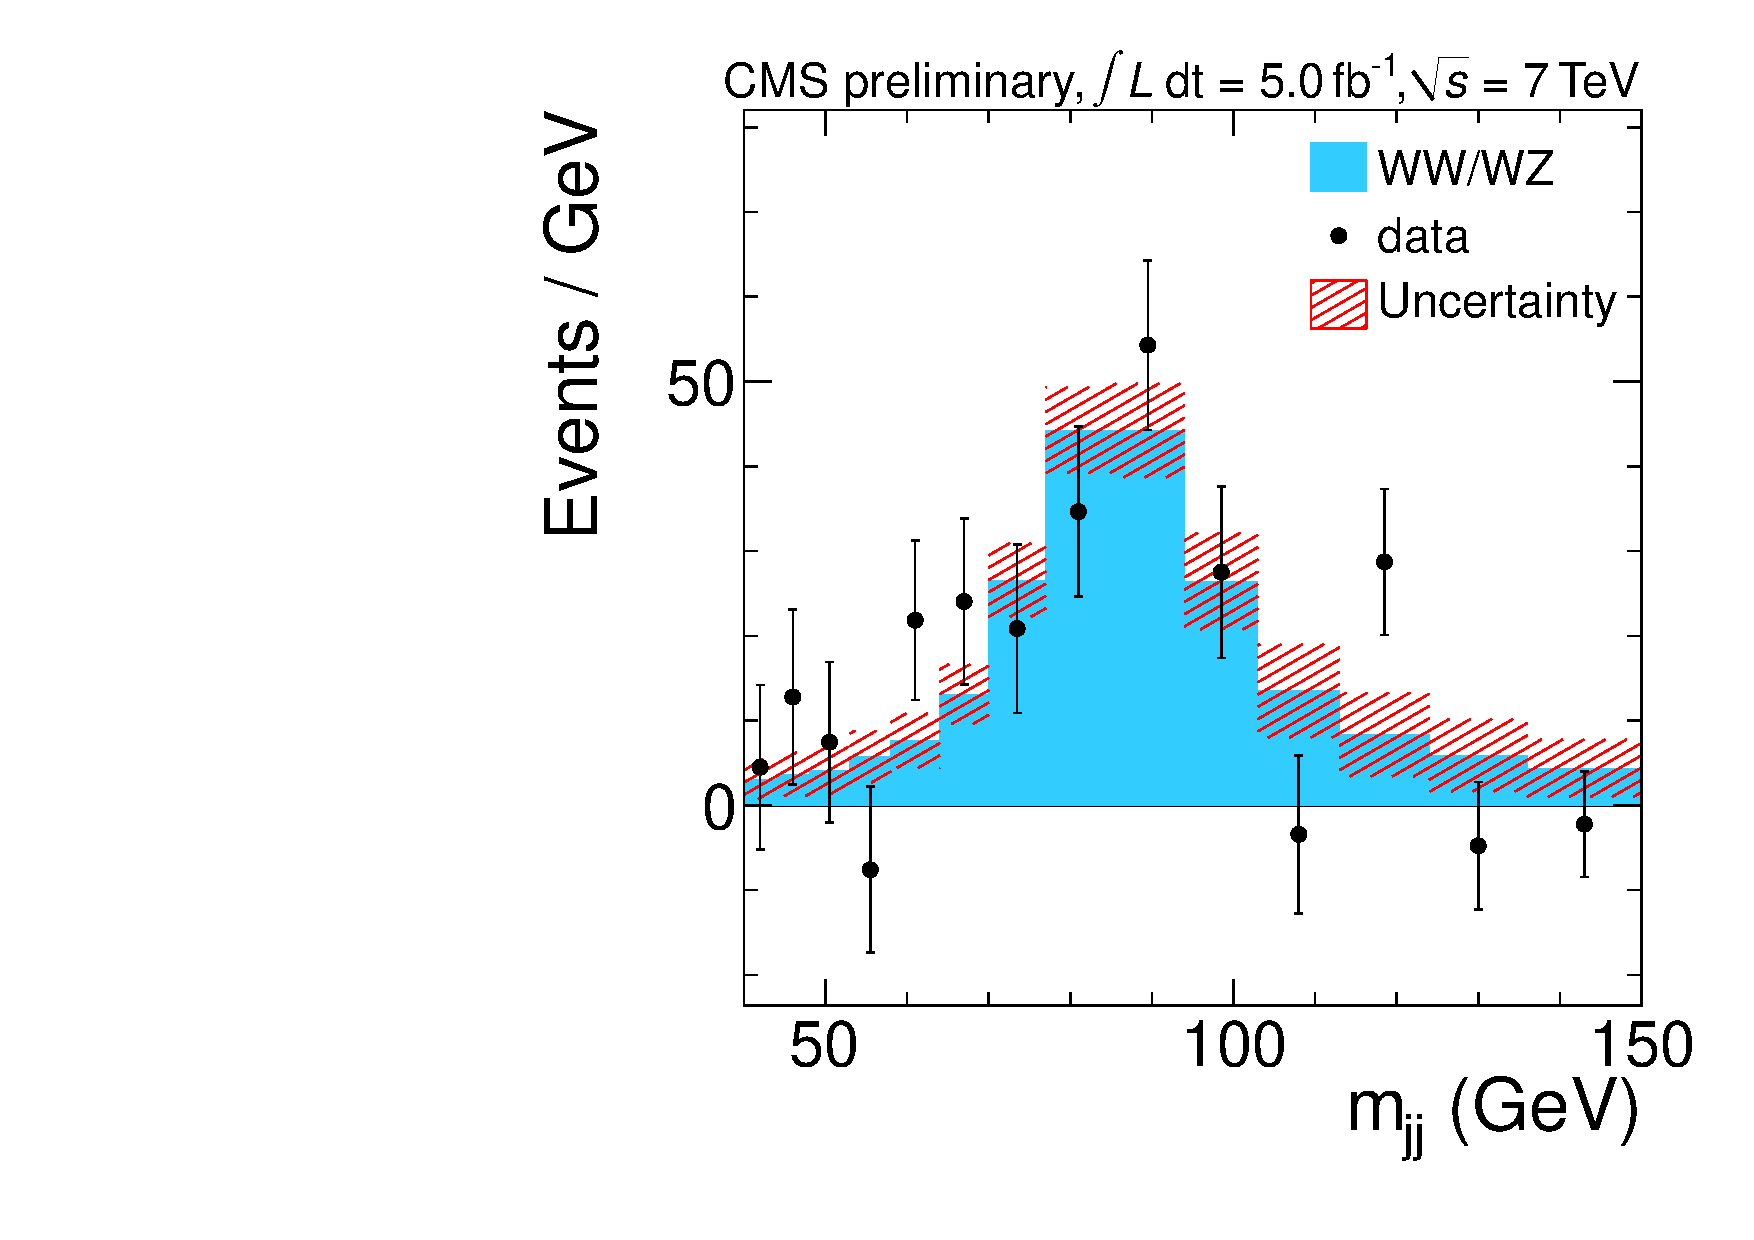
\includegraphics[width=0.49\textwidth]{figs/mjjfit_2jetsample/Wjj_Diboson_Muon_2jets_Subtracted.pdf}
    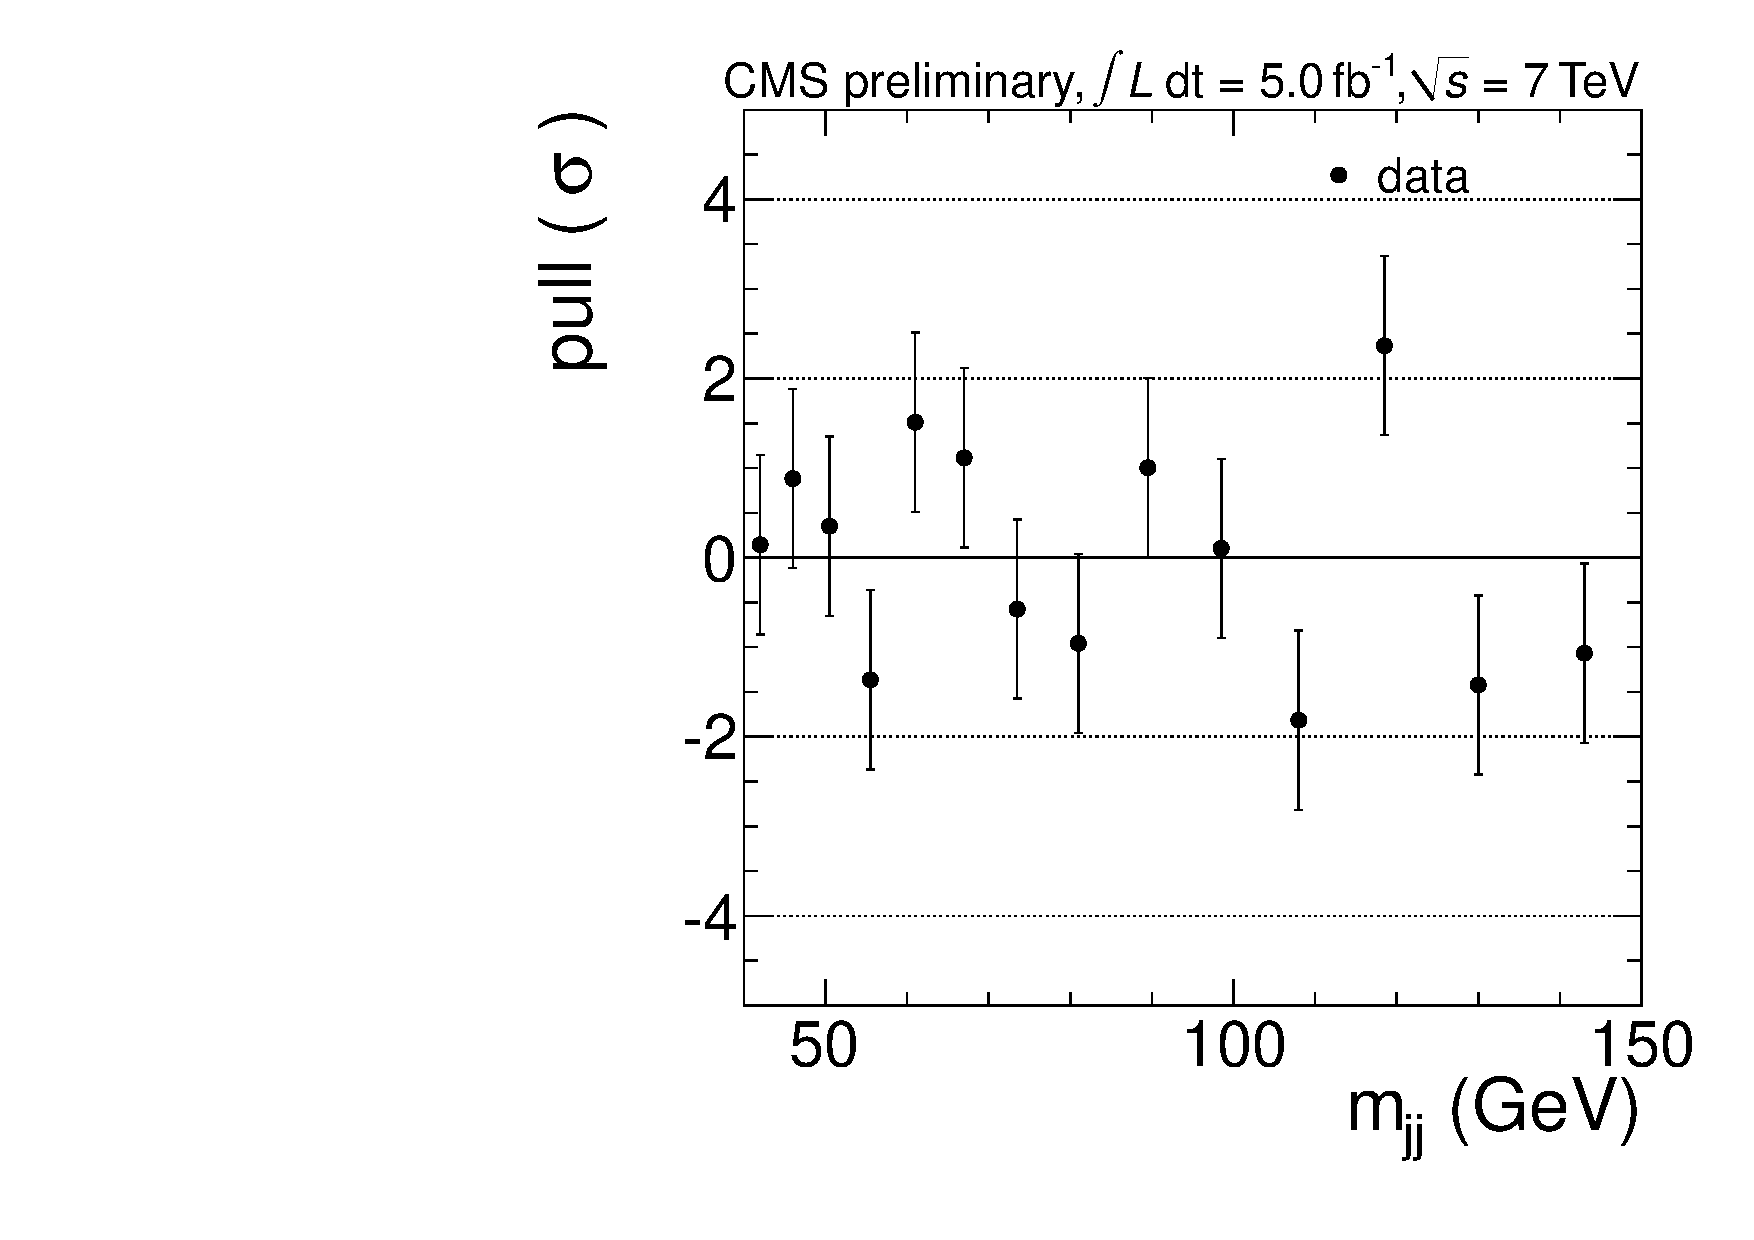
\includegraphics[width=0.49\textwidth]{figs/mjjfit_2jetsample/Wjj_Diboson_Muon_2jets_Pull.pdf}
    \caption{Distribution of the dijet invariant mass for the non-b-tagged 2-jet events in muon data and Monte Carlo: 
      (upper left) All background components stacked together, 
      (upper right) unstacked, (lower left) [Data minus all backgrounds except diboson],  
      (lower right) normalized residual between data and MC. The vertical dotted lines
      indicate the mass interval excluded from the fit.}
    \label{fig:mjj_2jet_mu}}
\end{figure}
%%%%%%%%%%%%%%%%%%%%
%%%%%%%%%%%%%%%%%%%%
\begin{figure}[h!]
  {\centering
    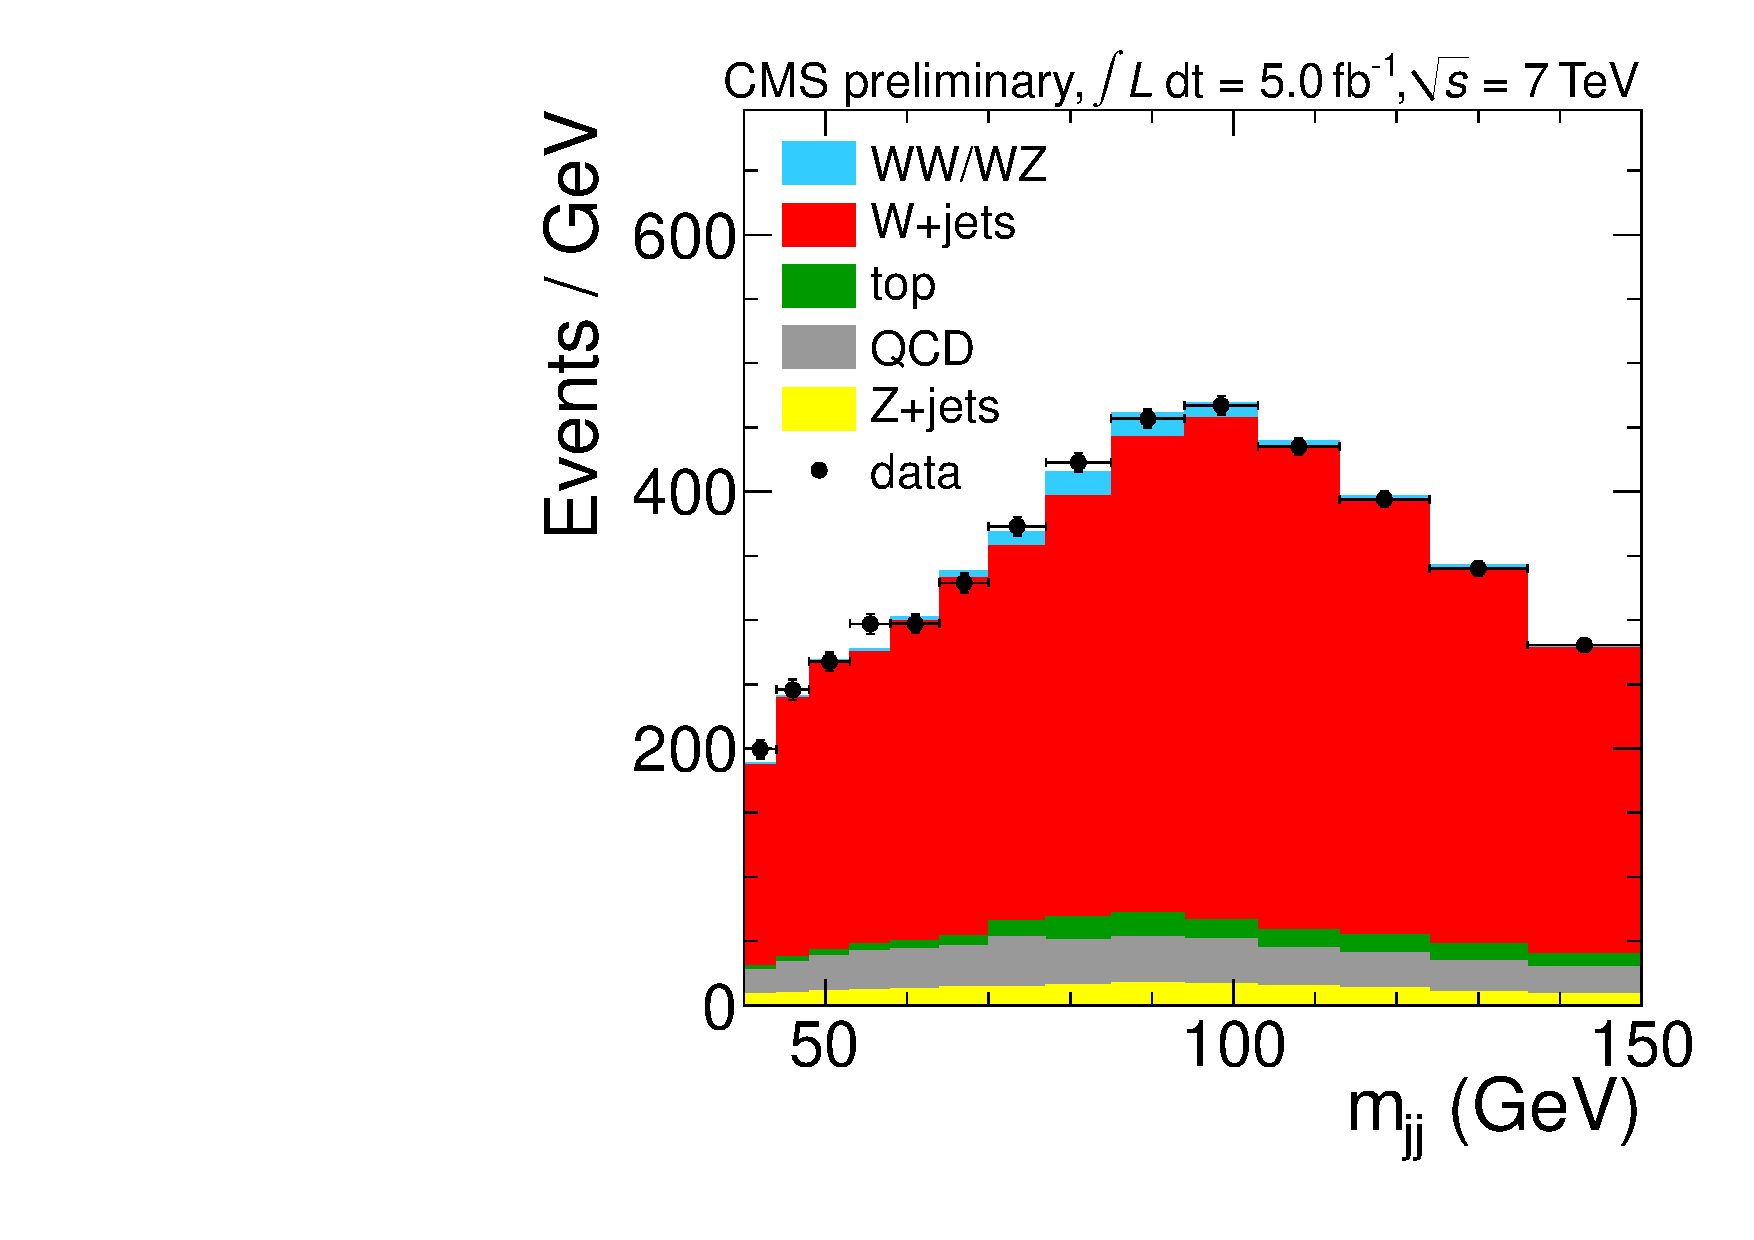
\includegraphics[width=0.49\textwidth]{figs/mjjfit_2jetsample/Wjj_Diboson_Electron_2jets_Stacked.pdf}
    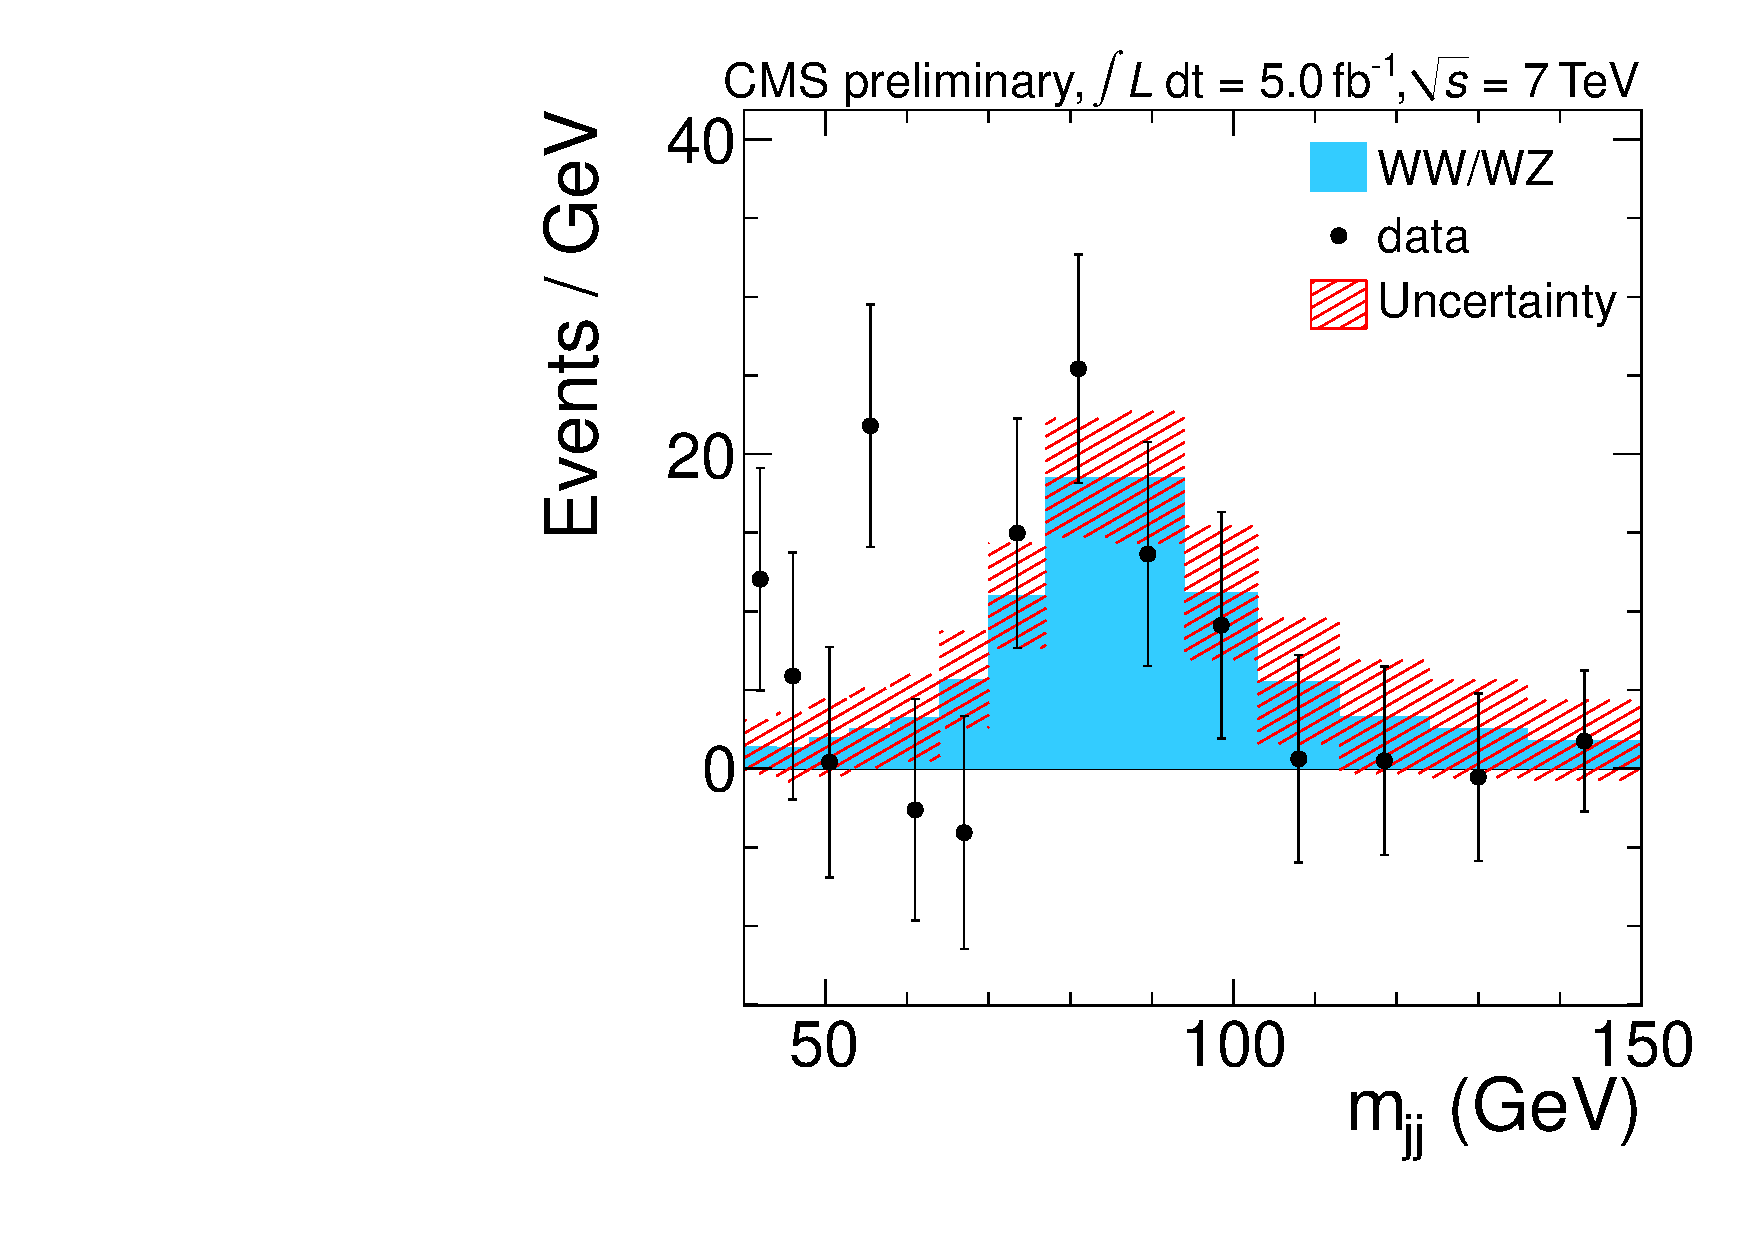
\includegraphics[width=0.49\textwidth]{figs/mjjfit_2jetsample/Wjj_Diboson_Electron_2jets_Subtracted.pdf}
    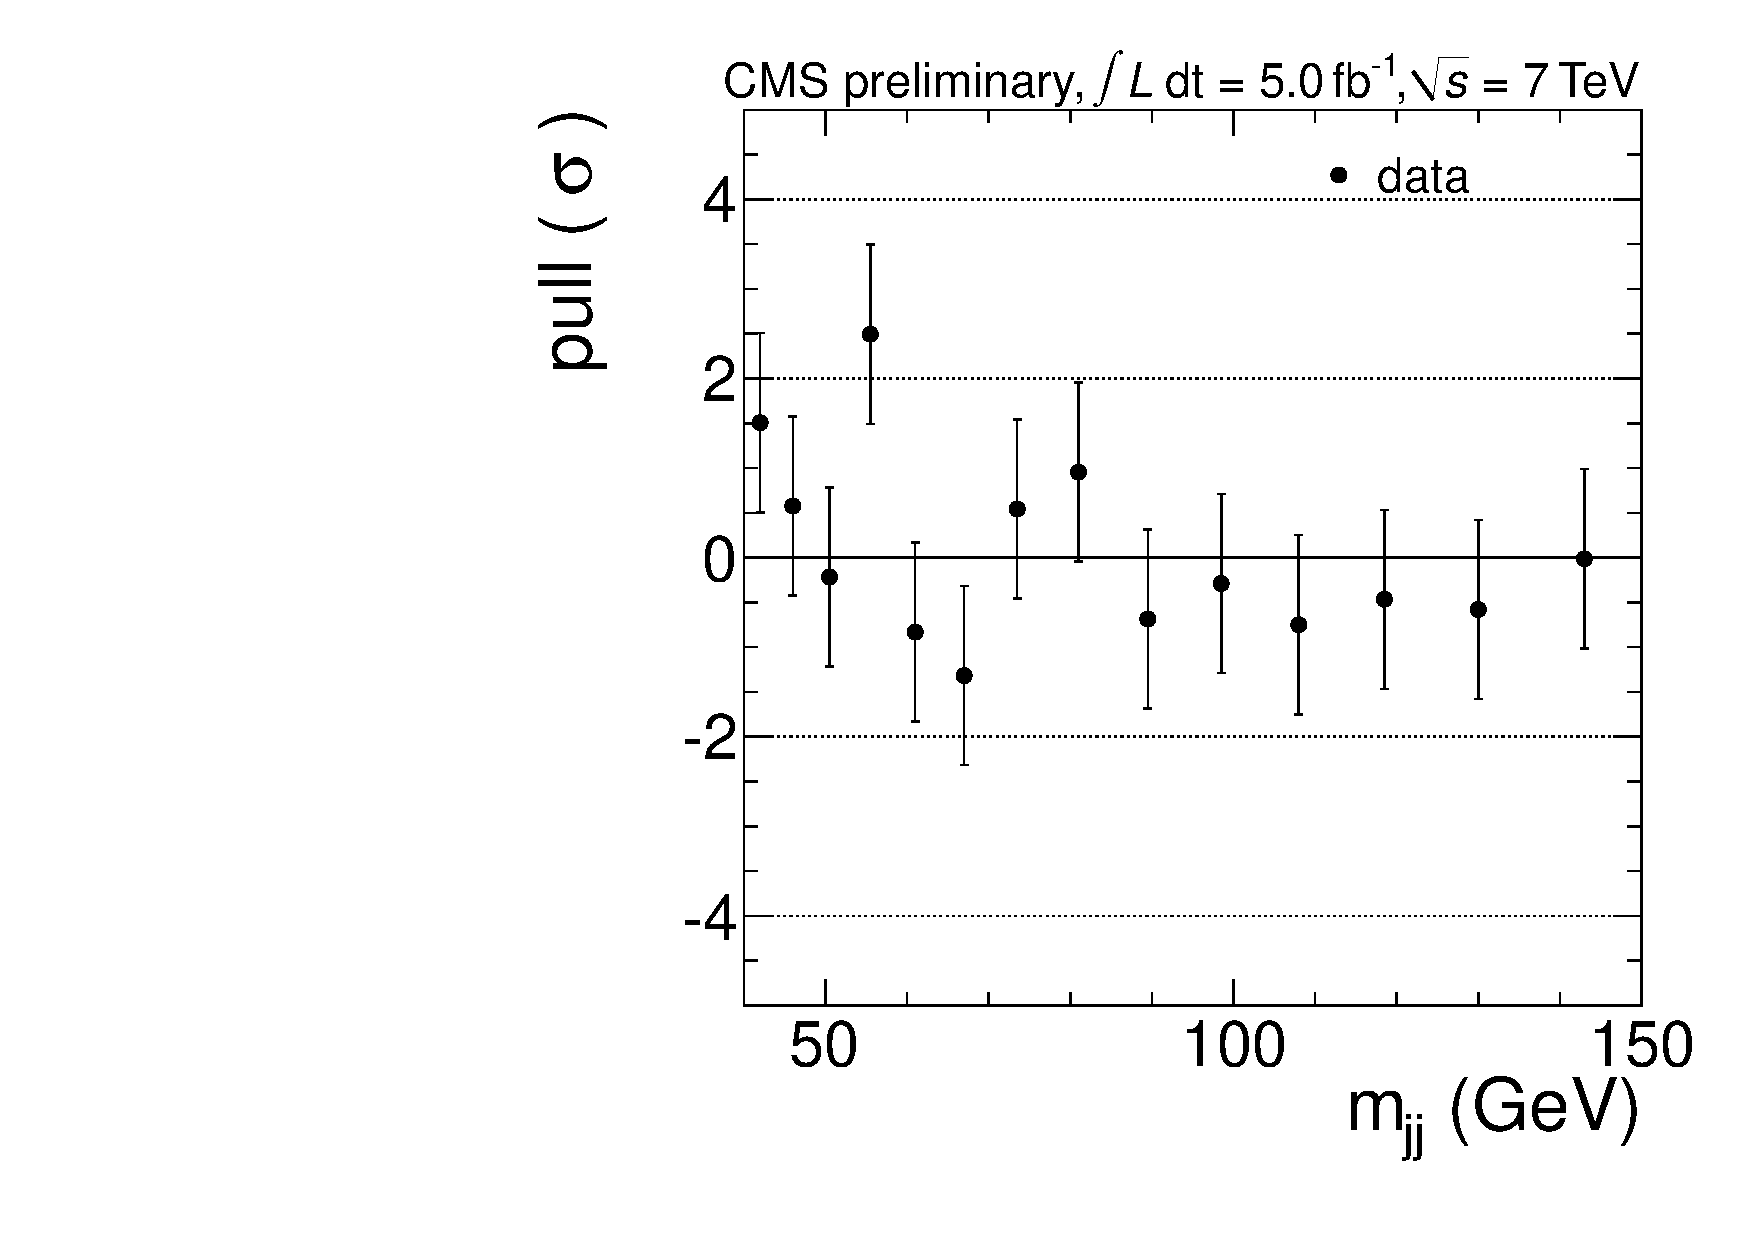
\includegraphics[width=0.49\textwidth]{figs/mjjfit_2jetsample/Wjj_Diboson_Electron_2jets_Pull.pdf}
    \caption{Distribution of the dijet invariant mass for the non-b-tagged 2-jet events in electron data and Monte Carlo: 
      (upper left) All background components stacked together, 
      (upper right) unstacked, (lower left) [Data minus all backgrounds except diboson],  
      (lower right) normalized residual between data and MC. The vertical dotted lines
      indicate the mass interval excluded from the fit.}
    \label{fig:mjj_2jet_el}}
\end{figure}
%%%%%%%%%%%%%%%%%%%%
%%%%%%%%%%%%%%%%%%%%
\begin{figure}[h!]
  {\centering
    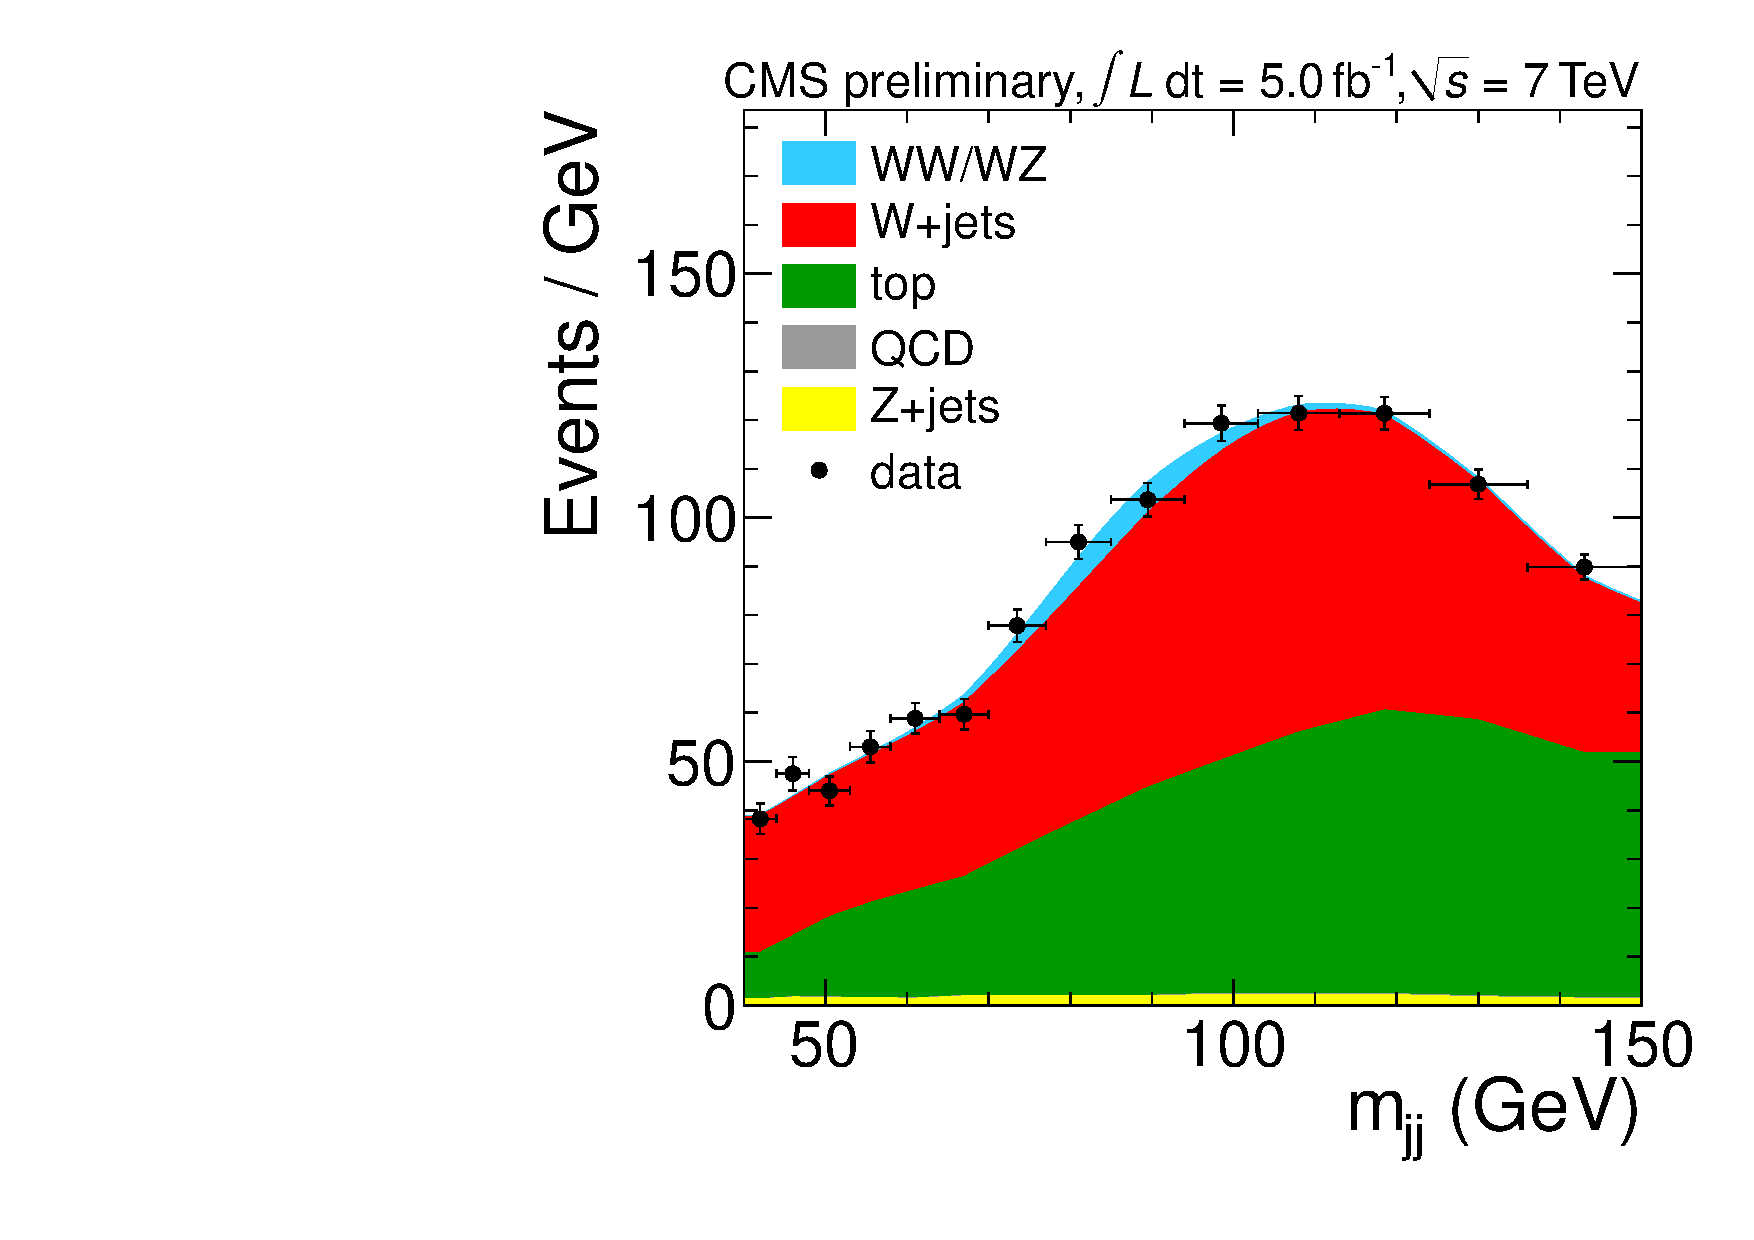
\includegraphics[width=0.49\textwidth]{figs/mjjfit_2jetsample/Wjj_Diboson_btag_Muon_2jets_Stacked.pdf}
    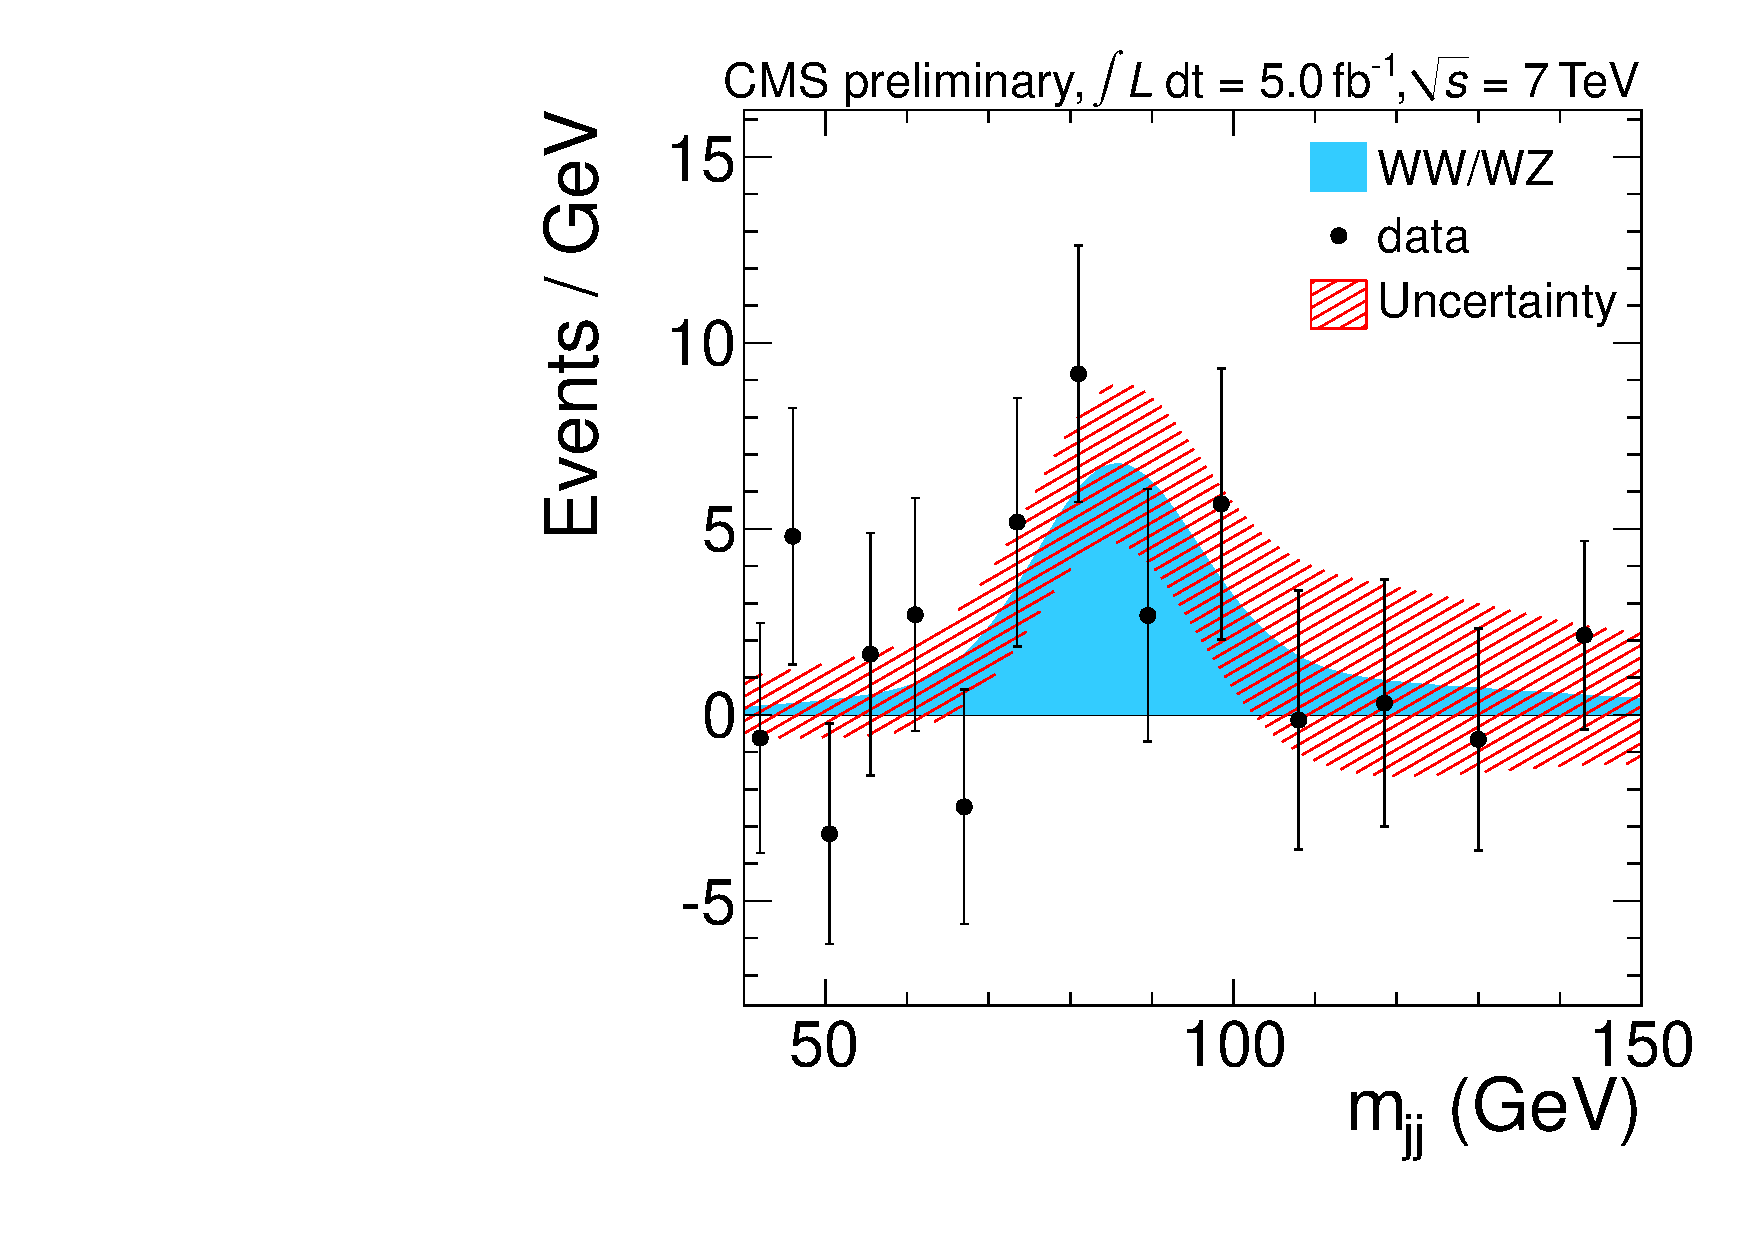
\includegraphics[width=0.49\textwidth]{figs/mjjfit_2jetsample/Wjj_Diboson_btag_Muon_2jets_Subtracted.pdf}
    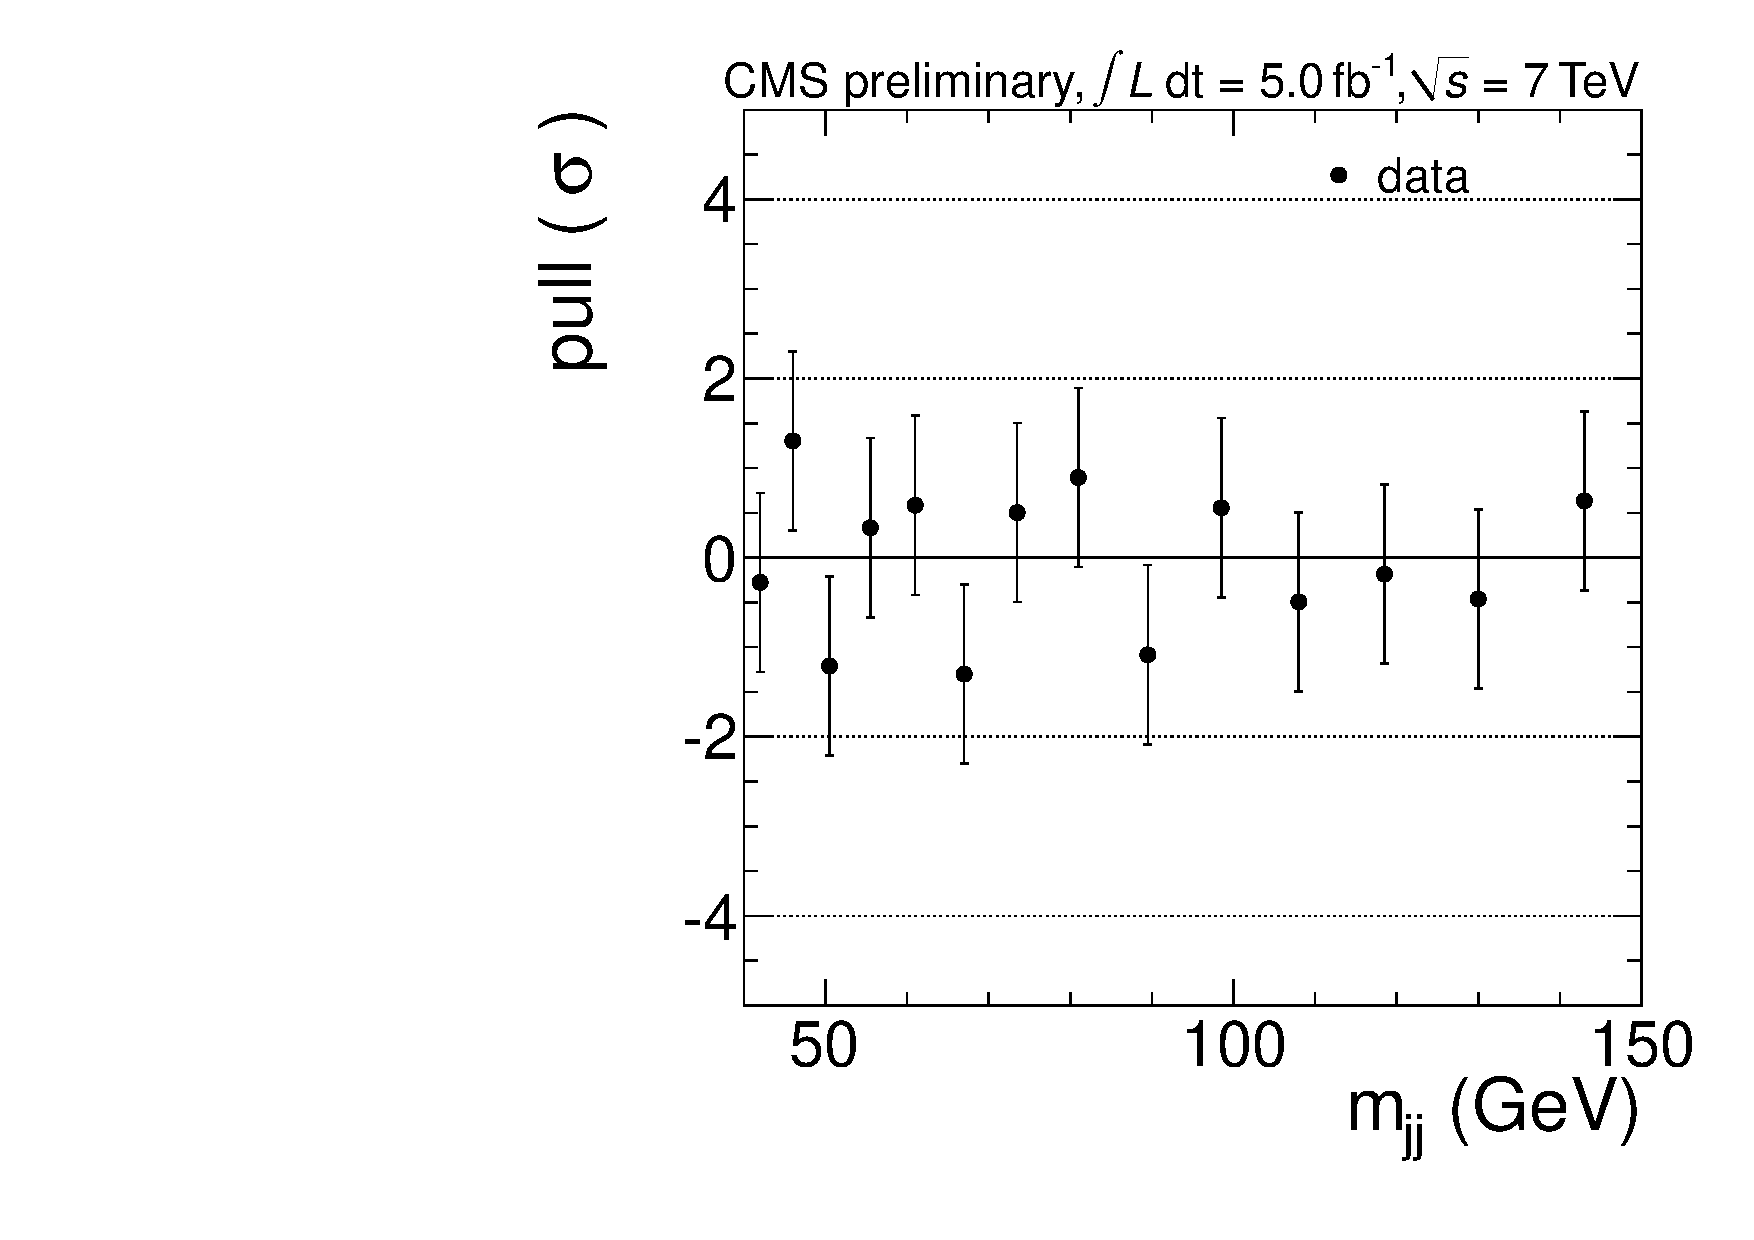
\includegraphics[width=0.49\textwidth]{figs/mjjfit_2jetsample/Wjj_Diboson_btag_Muon_2jets_Pull.pdf}
    \caption{Distribution of the dijet invariant mass for the b-tagged 2-jet events in muon data and Monte Carlo: 
      (upper left) All background components stacked together, 
      (upper right) unstacked, (lower left) [Data minus all backgrounds except diboson],  
      (lower right) normalized residual between data and MC. The vertical dotted lines
      indicate the mass interval excluded from the fit.}
    \label{fig:mjj_2jet_mu_btag}}
\end{figure}
%%%%%%%%%%%%%%%%%%%%
%%%%%%%%%%%%%%%%%%%%
\begin{figure}[h!]
  {\centering
    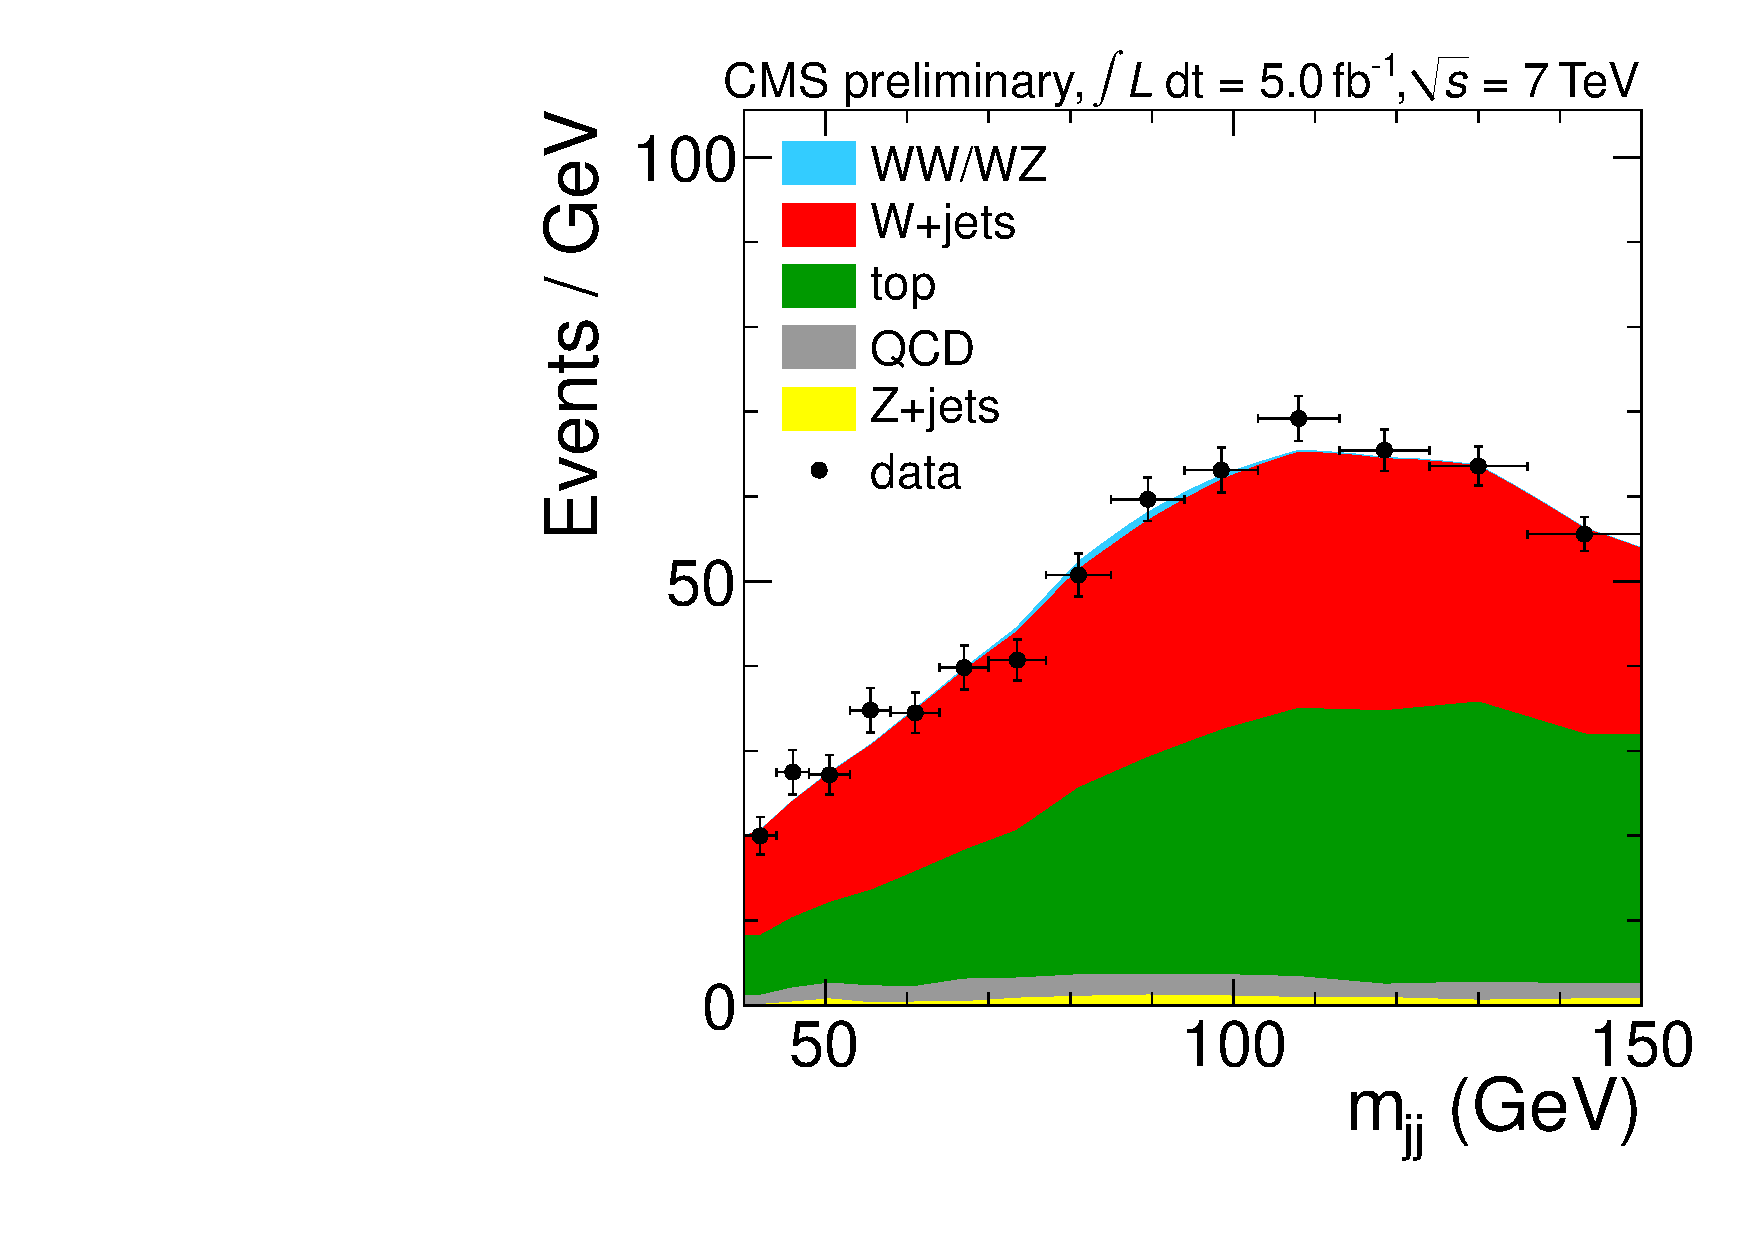
\includegraphics[width=0.49\textwidth]{figs/mjjfit_2jetsample/Wjj_Diboson_btag_Electron_2jets_Stacked.pdf}
    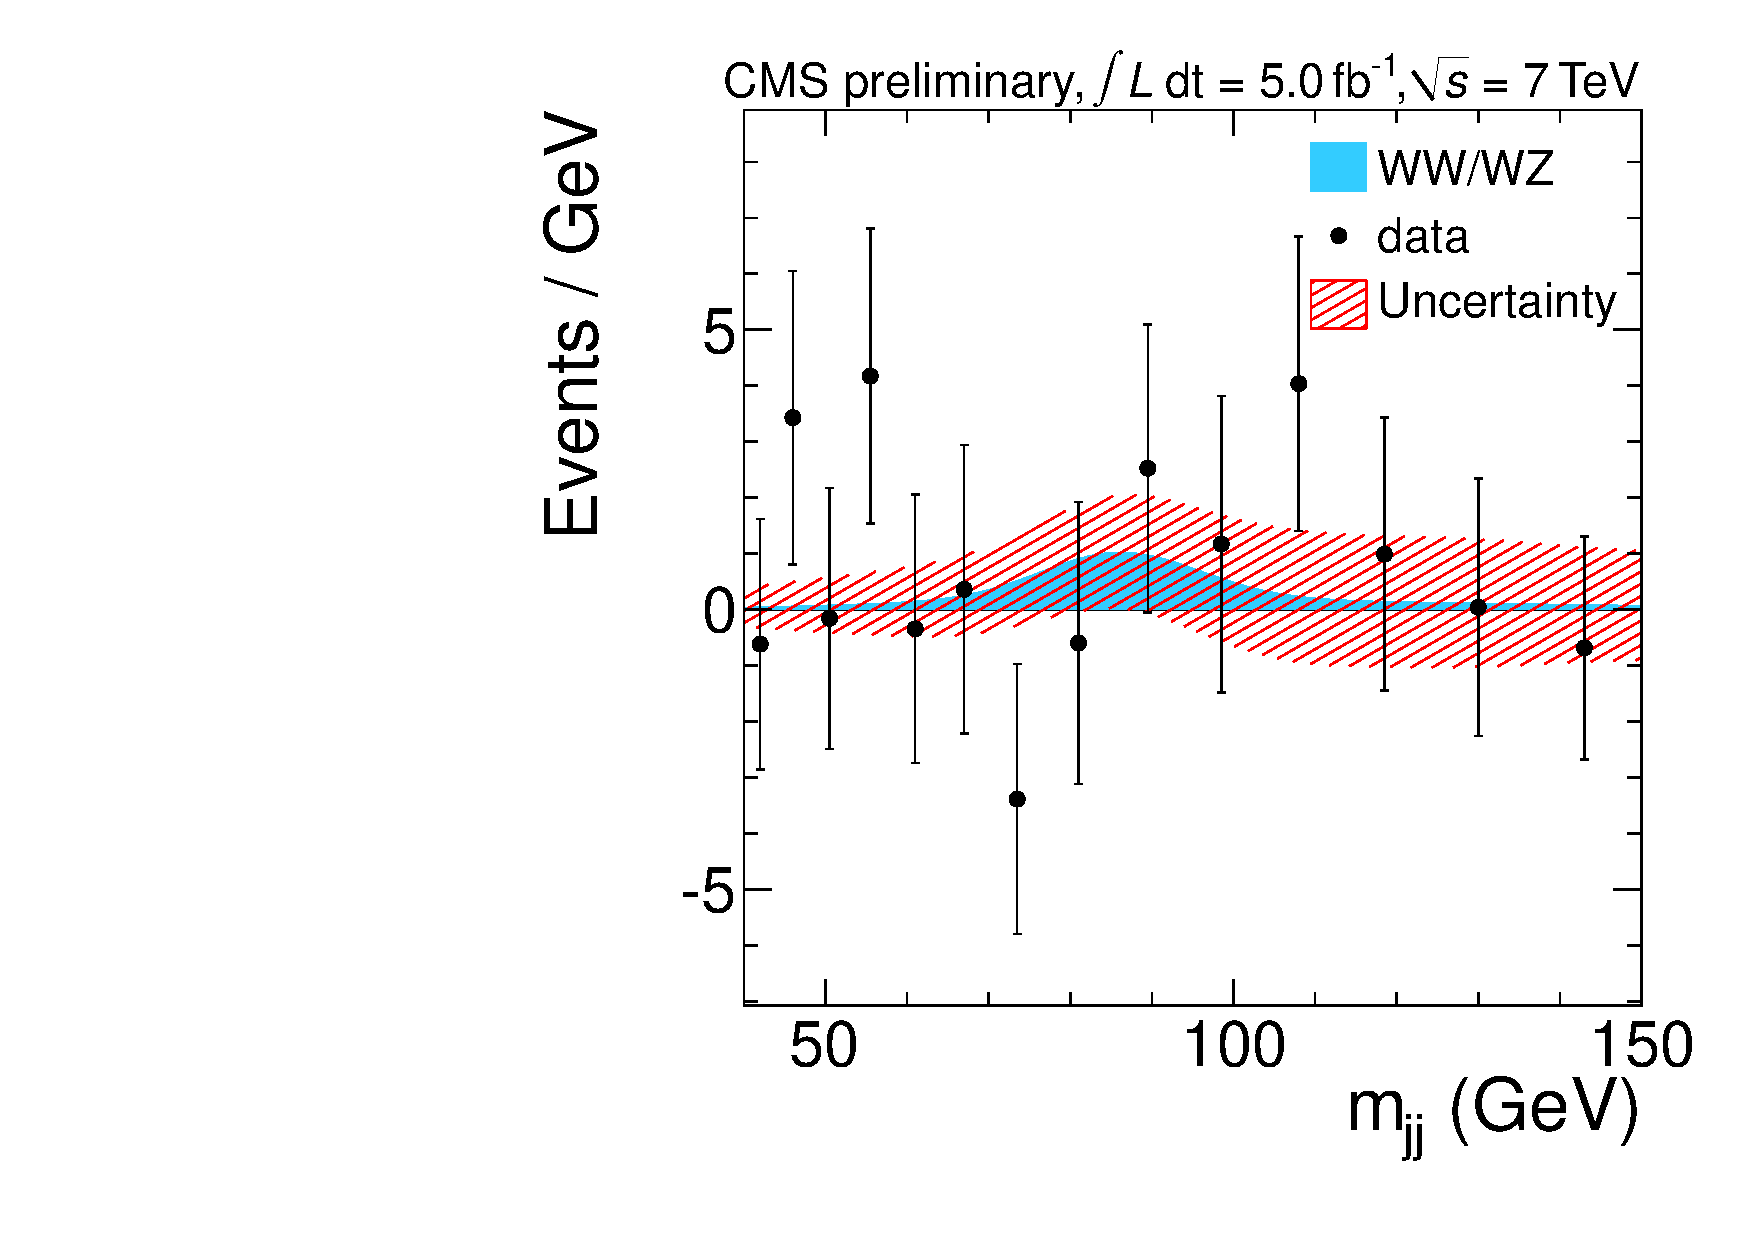
\includegraphics[width=0.49\textwidth]{figs/mjjfit_2jetsample/Wjj_Diboson_btag_Electron_2jets_Subtracted.pdf}
    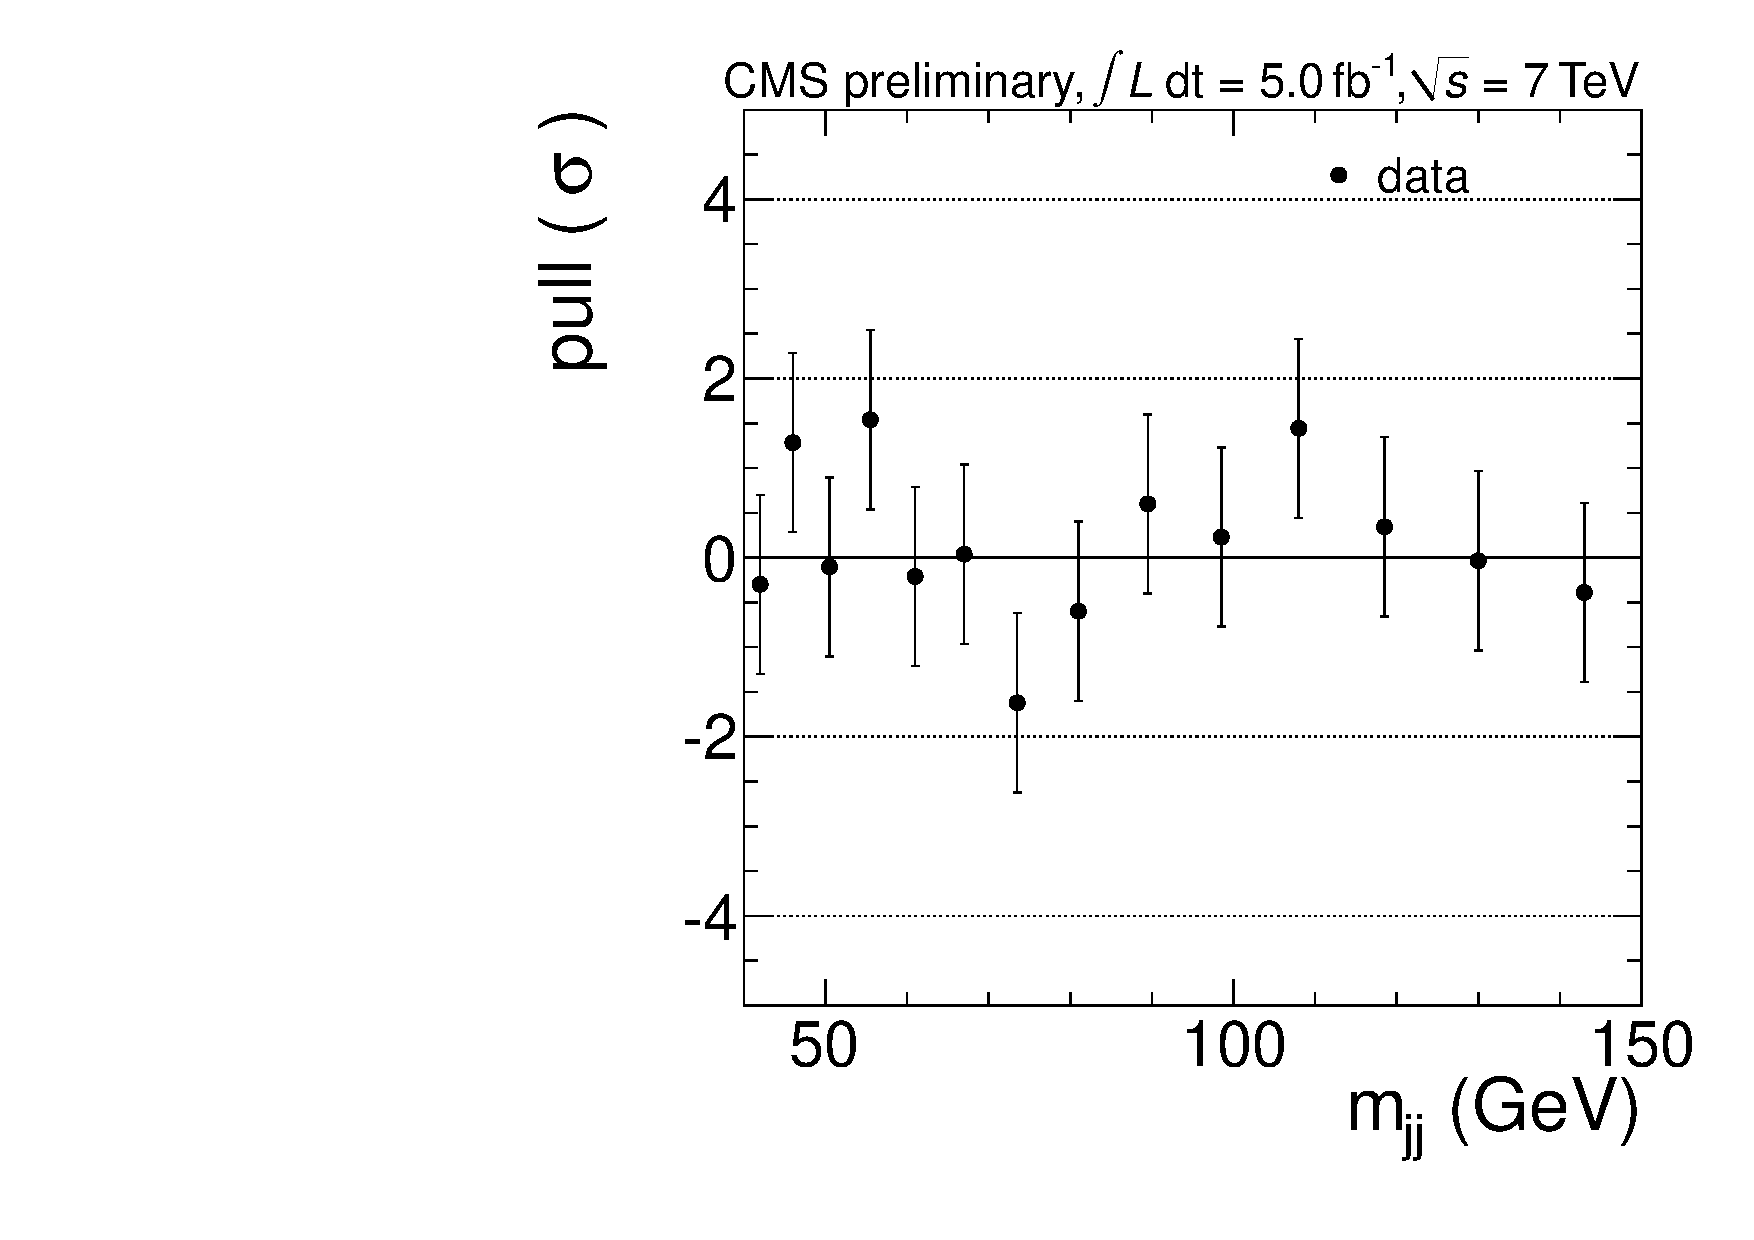
\includegraphics[width=0.49\textwidth]{figs/mjjfit_2jetsample/Wjj_Diboson_btag_Electron_2jets_Pull.pdf}
    \caption{Distribution of the dijet invariant mass for the b-tagged 2-jet events in electron data and Monte Carlo: 
      (upper left) All background components stacked together, 
      (upper right) unstacked, (lower left) [Data minus all backgrounds except diboson],  
      (lower right) normalized residual between data and MC. The vertical dotted lines
      indicate the mass interval excluded from the fit.}
    \label{fig:mjj_2jet_el_btag}}
\end{figure}
%%%%%%%%%%%%%%%%%%%%
%%%%%%%%%%%%%%%%%%%%
%%%%%%%%%%%%%%%
%%%%%%%%%%%%%%%
\begin{table}[tbht!]
\begin{center}
\caption{Event yields determined from a likelihood fit to the data, their expected values and the Diboson Yield corrected for the fit bias.}
 \label{table:FitTotalsAndComparisons}
\vspace{0.5cm}
 \begin{tabular} {l  c  c c c }
   \hline \hline
Bin            &  \multicolumn{2}{c}{Muons, non-b-tagged} & \multicolumn{2}{c}{Electrons, non-b-tagged} \\  
\hline
               & Predicted &   Extracted     &  Predicted &  Extracted \\
\hline
Dibosons       &   1697    &  1736 $\pm$ 389 &    867     &  727 $\pm$ 302 \\
Multijet       &    123    &   119 $\pm$ 317 &   2610     & 3204 $\pm$ 867 \\
Single Top     &    653    &   652 $\pm$ 33  &    332     &  332 $\pm$  17 \\
$\ttbar$       &   1679    &  1666 $\pm$ 117 &    963     &  953 $\pm$  67 \\
W+Jets         &  76129    & 67674 $\pm$ 586 &  37137     & 32706 $\pm$ 850 \\
Drell-Yan+Jets &   3610    &  3613 $\pm$ 155 &   1487     &  1485 $\pm$ 64 \\
Total Yields   &  83891    &  75460          &  43396     &  39407 \\ 
\hline 
Corrected Diboson & 1697   &   1899$\pm$389  &    867     &   783$\pm$302  \\
\hline 
Data           &    ---    &  75419          &    ---     &  39365 \\ 
\hline
\\
\hline
\hline
Bin            &  \multicolumn{2}{c}{Muons, b-tagged} & \multicolumn{2}{c}{Electrons, b-tagged} \\  
\hline
               & Predicted &   Extracted     &  Predicted &  Extracted \\
\hline
Diboson        &    211    &   226 $\pm$ 203 &    110     &   35 $\pm$ 86 \\
Multijet       &     16    &    16 $\pm$ 42  &    171     &  231 $\pm$ 78 \\
Single Top     &   1220    &  1219 $\pm$ 60  &    618     &  626 $\pm$ 31 \\
$\ttbar$       &   3206    &  3192 $\pm$ 191 &   1846     & 1976 $\pm$ 104 \\
W+Jets         &   5082    &  5082 $\pm$ 206 &   2551     & 2693 $\pm$ 107 \\
Drell-Yan+Jets &    206    &   206 $\pm$ 9   &    857     &   858 $\pm$ 37 \\
Total Yields   &    9941   &  9941          &    6153     &  5648 \\ 
\hline 
Corrected Diboson &    211 &    247$\pm$203  &    110     &    38$\pm$86  \\
\hline 
Data           &    ---    &  9940          &    ---      &  5695 \\ 
\hline \hline
\end{tabular}
\end{center}
\end{table}

\begin{table}[bthp]
\begin{center}
\caption{\label{tab:dibosonYield} Diboson signal yields with the statistical contribution and the systematic contribution to the uncertainties broken out.  The first uncertainty arises chiefly from statistics the second is from systematic sources.}
\begin{tabular}{rcc}
\hline\hline
& muons, non-b-tagged & electrons, non-b-tagged \\
\hline
Diboson & $1899 \pm 275 \pm 275$ & $795 \pm 198 \pm 227$ \\
\hline
& muon, b-tagged & electrons, non-b-tagged \\
\hline
Diboson & $247 \pm 100 \pm 176$ & $38 \pm 75 \pm 42$ \\
\hline\hline
\end{tabular}
\end{center}
\end{table}
%%%%%%%%%%%%%%%
%%%%%%%%%%%%%%%
%%%%%%%%%%%%%%%%%%%%%%%%%%%%%%%%%%%%%%%%%%%%%%%%%%%%%%%%%%%%


%%%%%%%%%%%%%%%%%%%%%%%%%%%%%%%%%%%%%%%%%%%%%%%%%%%%%%%%%%%%
%%%%%%%%%%%%%%%%%%%%%%%%%%%%%%%%%%%%%%%%%%%%%%%%%%%%%%%%%%%%
\clearpage
\subsection{Fit Validation}

We verify that the signal extraction procedure is unbiased and that 
statistical uncertainties reported have good coverage by constructing
and fitting toy datasets. Since our fit procedure is the same in both
electron and muon channels, we validate and perform a number of cross-checks
using muons; with the electron results subsequently listed. 
The specific steps are:
\begin{enumerate}
\item Perform the default fit and obtain the expected yields 
(Table~\ref{table:FitValidation_mu_NoBTag}).
\item Generate toy Monte Carlo for each process from the corresponding MC distributions.
\item Construct 1000 sample datasets. The excpected yield are first smeared by the fit 
errors, with correlations taken into account, by computing the errors in a coordinate frame 
where they are uncorrelated and rotating back (Sec.~\ref{sec:FitValidation_ExpectedEventGeneration}). 
Afterwards, we smear the expected yields by the Poisson Errors.
\item Perform the fit for each sample dataset.
\item Examine the resultant Yields and Pulls.
\end{enumerate}


\subsubsection{Expected Event Generation}
\label{sec:FitValidation_ExpectedEventGeneration}
Due to the constraints imposed by the data, the fitted event yields are strongly correlated
(Sec.~\ref{sec:mjj_2jetfit}). This fact is taken into account 
when smearing the expected values. In short we perform a transformation to 
the coordinate system where the yields are uncorrelated, smear and transform back. Specifically,
for each toy dataset we:
\begin{enumerate}
\item Diagonalize the Covariance Matrix ($\Sigma$) obtained from the original fit to the 
data (Sec.~\ref{sec:mjj_2jetfit}). I.e. find $M$ such that $M\Sigma M^{-1}$ is 
diagonal (Rows of $M$ are in fact the eigenvectors of $\Sigma$).
\item Produce the errors ($z_i$) in a frame where there is no correlation between the fitted 
'yields' (i.e. in a frame where the Covariance Matrix is diagonal). Namely, $z_i$ are randomly 
selected from a Gaussian distribution with $\sigma_i^2=(M\Sigma M^{-1})_{ii}$ and mean$=0$.
\item Transform back to the orignal frame and obtain the yields ($x_i$) smeared by the fit error: 
$x_i=\mu_i+(M^{-1}Z)_i$, where $\mu$ is the expected value from the default fit.
\item Poisson-smear $x_i$ and generate the dataset with the obtained values.
\item Perform the fit.
\end{enumerate}


\subsubsection{Diboson Fit Validation}
The bias and pull distributions for the Diboson are shown in
Fig~\ref{fig:DibosonValidation_mu_NoBTag},
with gaussian fit parameters are given in
Table~\ref{table:FitValidation_mu_NoBTag}. It should be noted that
we have a significant correlation
between the Diboson and W+Jets yields (Sec.~\ref{sec:mjj_2jetfit}) (as well as a limited amount
of Monte Carlo, particularly in the case of alternate choices of W+Jets scale and matching).
On average, the fitter returns a diboson event count which is $1.094$ times ($163$ evts.) higher 
than expected. As described in Section~\ref{sec:FitValidation_fixedfMUfSU}, the shift is a result of 
allowing the relative fractions
of the alternate (factorization and matching) samples to float during fitting.
The fit error is accurately estimated. The fitted yields after correcting for the corresponding biases
 are listed in Table~\ref{table:BiasCorrectedFitTotalsAndComparisons}.


%%%%%%%%%%%%%%%
\begin{table}[tbht!]
\begin{center}
\caption{Event yields determined from a likelihood fit to the data and corrected for the fit bias.}
 \label{table:BiasCorrectedFitTotalsAndComparisons}
\vspace{0.5cm}
 \begin{tabular} {l  c  c c c }
   \hline \hline
Bin            &  \multicolumn{2}{c}{Muons, non-b-tagged} & \multicolumn{2}{c}{Electrons, non-b-tagged} \\  
\hline
               & Predicted &   Extracted     &  Predicted &  Extracted \\
\hline
Dibosons       &   1697    &   1899          &    867     &  783 \\
Multijet       &    123    &   296           &   2610     &  4195  \\
Single Top     &    653    &   650           &    332     &  308 \\
$\ttbar$       &   1679    &   1662          &    963     &  946  \\
W+Jets         &  76129    &   67384         &  37137     &  31644 \\
Drell-Yan+Jets &   3610    &   3609          &   1487     &  1408 \\
Total Yields   &  83891    &   75420         &  43396     &  39371 \\ 
\hline 
Data           &    ---    &   75419         &    ---     &  39365 \\ 
\hline \hline
\end{tabular}
\end{center}
\end{table}
%%%%%%%%%%%%%%%

\subsubsection{Non-Diboson Parameters}
For reference, we examine all of the variables allowed to float in the fit (Figs.~\ref{fig:Validation_Yields_mu_NoBTag_2j},~\ref{fig:Validation_Pulls_mu_NoBTag_2j}). 
The results are summarized in Table~\ref{table:FitValidation_mu_NoBTag}, where
the variation in the gaussian widths is due to differing
constraints imposed when fitting
(Table~\ref{tab:mjj_shapes_and_normalization}). Besides QCD (which is difficult 
to model \& validate and has a large correlation with W+Jets), 
the yields returned by the fitter are consistent with the
expectation within a few percent. Since the W+Jets shape, as well as its yield, 
are able to vary we obtain a somewhat more centered pull values 
($\sigma_{Pull}=0.8$). Likewise, a large degree of correlation allows the Diboson
to compensate for the discrepancies between given and extracted W+Jets counts thus
leading to a very narrow ($\sigma<<1$) Total Pull Distribution.

The expected values and pulls for the fraction of Matrix Element -
Parton Shower Matching MC ($fMU$) and fraction of Factorization Scale
MC ($fSU$) in the W+jets sample are displayed in
Fig~\ref{fig:Validation_fMUfSU_mu_NoBTag_2j}.
As usual, $fMU<0$ ($fSU<0$) denotes the fact that we're using a
Matching Down (Scale Down) sample instead; which can lead to different
(pull and yield) distributions when these fractions are $>0$ vs
$<0$. Insufficient discriminating ability between Up and
Down templates (shown in
Fig~\ref{fig:Validation_fMUfSU_ShapeComparisonUpVsDown}) creates additional
challenges. However, as shown in the previous
section, the above complications do not have a major impact on the fit results and the (average) 
extracted Diboson Yield is within $\sim 10\%$ of the expected value.


\subsubsection{Electron Validation}
We repeat the above validation procedure for the electron fit. As expected, the results mirror those in the
 muon channel with strong correlations observed between Dibosons, W+Jets and QCD
values. Our fit underestimates the Diboson Yield by $\sim 8\%$, while accurately gauging the corresponding error (Fig.~\ref{fig:DibosonValidation_el_NoBTag}). 
The yield (pull) distributions for the remaining parameters are shown in Fig.~\ref{fig:Validation_Yields_el_NoBTag_2j} (Fig.~\ref{fig:Validation_Pulls_el_NoBTag_2j}). 
We correct for the corresponding biases and summarize the results in Table~\ref{table:BiasCorrectedFitTotalsAndComparisons}.


\subsubsection{Fixed Scaling And Matching Fractions}
\label{sec:FitValidation_fixedfMUfSU}
As was previously discussed (Sec.~\ref{sec:wjetsShapeMatchingQ2}), the default fit allows the relative
fractions of the samples generated with alternate Factorization and ME-PS Matching scales to float. In order to
examine the impact of this approach, we repeat the validation procedure with the relative fractions fixed
to their expected values (both when generating the 1000 toy datasets as well as when fitting). The corresponding
Yield and Pull distributions are shown in Figs.~\ref{fig:Validation_Yields_NoBTag_2j_fixedfMUfSU},
\ref{fig:Validation_Pulls_NoBTag_2j_fixedfMUfSU}. By keeping the fractions fixed we
are insuring that the shape of the W+Jets distribution is no longer allowed to vary and are reducing
the impact that the degeneracies \& limited statistics of the alternative samples have on our fit.
As a result, the bias in the W+Jets yield is significantly reduced, while the bias in the Diboson Yield 
(which is now $<2\%$) is essentially eliminated.


\subsubsection{Injecting Varying Diboson Yield}
As an additional cross-check we repeat the validation procedure by
\begin{enumerate}
\item Removing the fit error smearing. The yields from the data are only
 Poisson-smeared and then used when constructing the toy datasets.
\item Shifting the Diboson Yield within $20\%$ of the expected value. 
\end{enumerate}
Specifically, we inject $0.8\times$,$\0.9\times$,$1.0\times$,$1.1\times$,$1.2\times$ the default yield by
generating $1000$ toy datasets for each configuration and repeating the validation procedure. The Diboson
Yield and Pull Distributions are displayed in Fig.~\ref{fig:Validation_fixedCentralYields_Diboson_mu_NoBTag_2j}, while the bias vs injected amount is shown in
Fig.~\ref{fig:Validation_fixedCentralYields_BiasScan_mu_NoBTag_2j}. As can be observed, the bias remains constant in the current parameter range .


%%%%%%%%%%%%%%%%%%%%%%%%%%%%
%%%%%%%
\begin{table}[tb]
\caption{Validation Parameter Values}
\begin{center}
\begin{tabular}{|c|c|c|c|c|c|}
\hline
   Parameter
 & From Data
 & $\mu_{Fitted-Given}$
 & $\sigma_{Fitted-Given}$ 
 & Pull $\mu$
 & Pull $\sigma$ \cr
\hline
\vspace{-0.5cm} & & \cr
{Diboson} & $1735$ & $-163.0\pm 12.0$ & $373.6\pm 8.3$ & $-0.407\pm 0.031$ & $0.958\pm 0.022$  \cr
\hline
{W+jets} & $67674$ & $289.9\pm 14.8$ & $460.4\pm 11.3$ & $0.494\pm 0.025$ & $0.789\pm 0.020$  \cr 
\hline
{Z+jets} & $3614$ & $3.9\pm 5.5$ & $172.1\pm 4.3$ & $0.030\pm 0.036$ & $1.108\pm 0.028$  \cr 
\hline
{Total} & $75460$ & $40.0\pm 0.1$ & $3.0\pm 0.1$ & $0.144\pm 0.000$ & $0.012\pm 0.000$  \cr 
\hline
{$t\bar{t}$} & $1666$ & $3.5\pm 3.9$ & $119.520\pm 3.134$ & $0.011\pm 0.034$ & $1.034\pm 0.026$  \cr 
\hline
{SingleTop} & $652$ & $2.0\pm 1.3$ & $39.749\pm 1.017$ & $0.044\pm 0.040$ & $1.251\pm 0.032$  \cr 
\hline
{$fMU$} & $-0.075$ & $-0.082\pm 0.002$ & $0.074\pm 0.002$ & $-1.247\pm 0.037$ & $1.140\pm 0.026$  \cr
\hline
{$fSU$} & $0.053$ & $-0.210\pm 0.003$ & $0.104\pm 0.003$ & $-3.238\pm 0.054$ & $1.634\pm 0.041$  \cr
\hline
\end{tabular}
\end{center}
\caption{The first column shows inputs to generate pseudo experiments for the muon fit validation studies, while the next two show the (fitted) mean and sigma for the 1000 Toy experiments.} 
\label{table:FitValidation_mu_NoBTag}
\end{table}
%%%%%%%


%%%%%%%%%%%%%%%%%%%%%%%%%%%%
%%%%%%%
\begin{figure}[h!] {\centering
\unitlength=0.33\linewidth
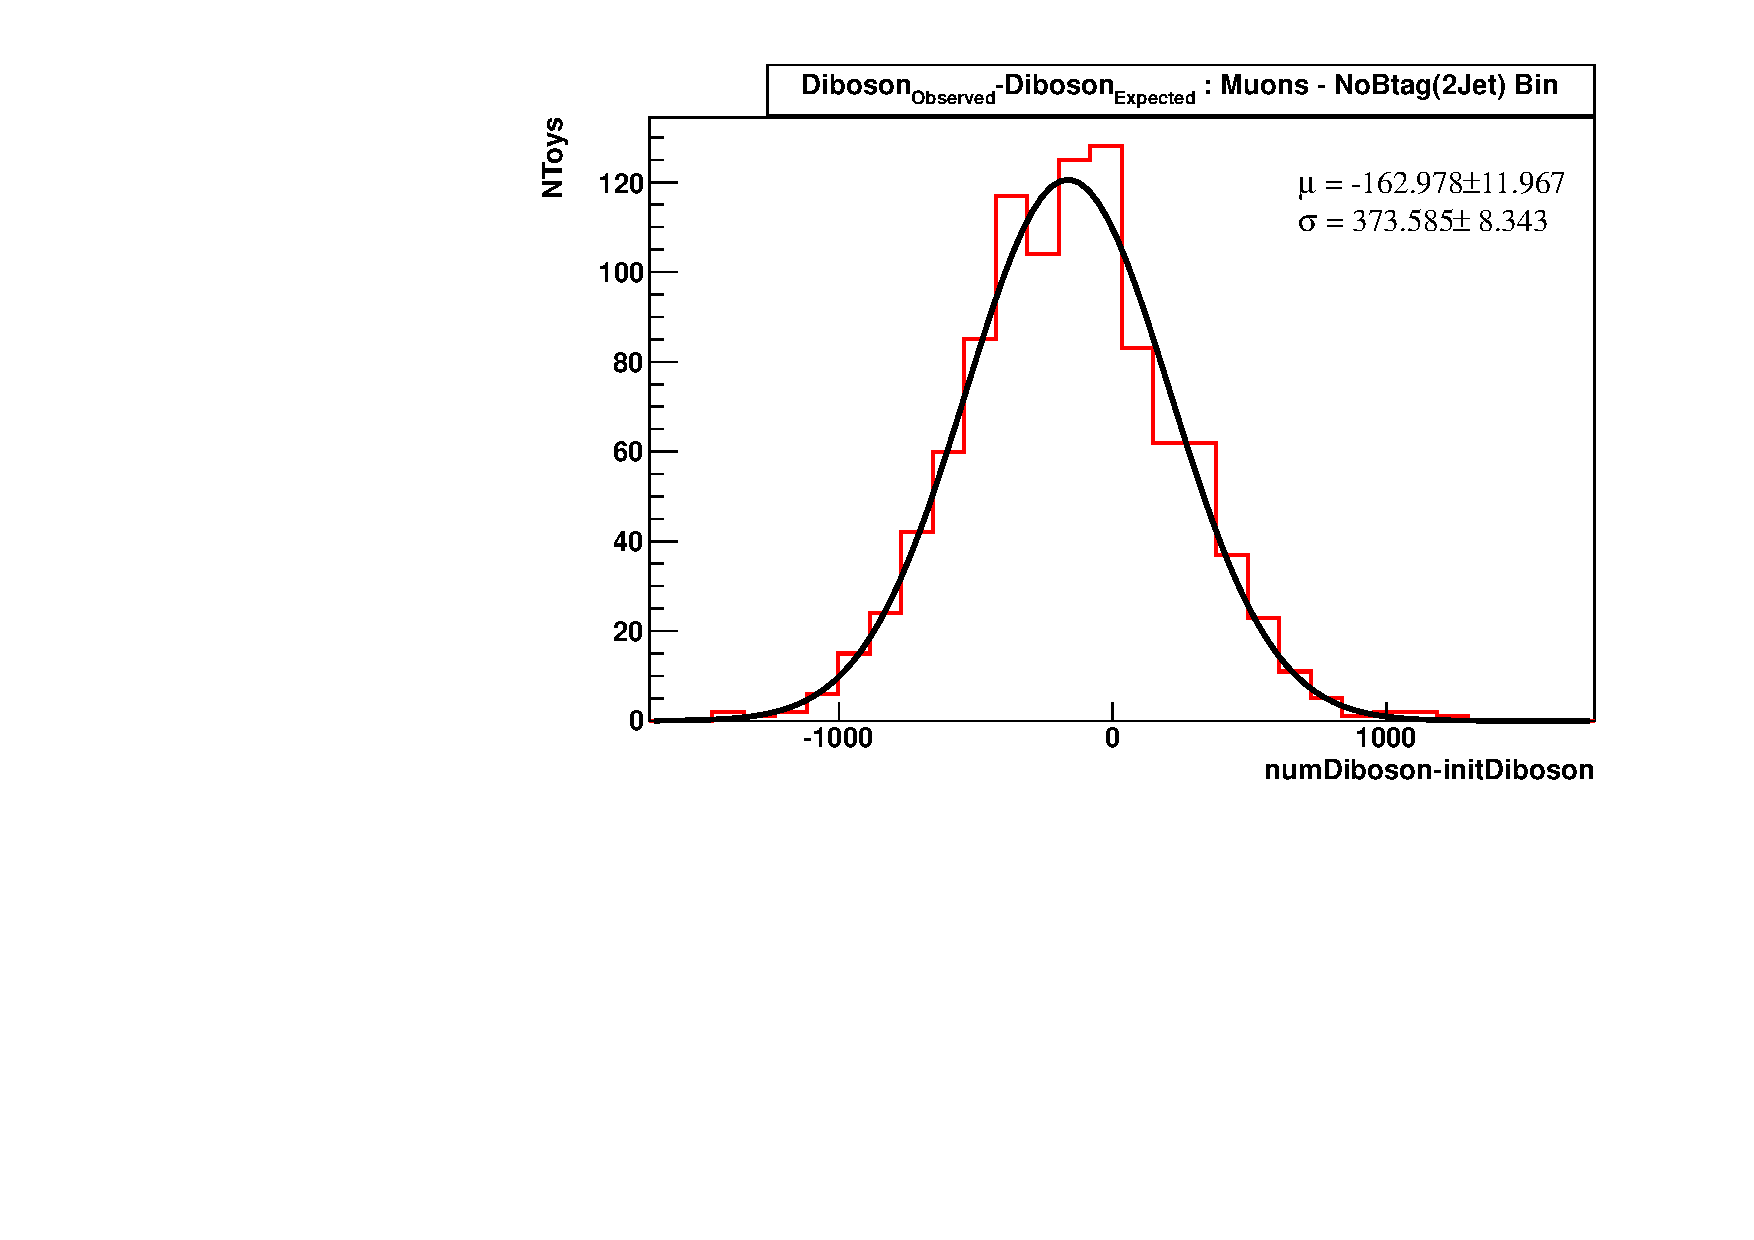
\includegraphics[width=0.96\textwidth]{figs/validation/DibosonYield_Validation_mu_NoBtag_2j.pdf}
\put(-1.5,0.0){(a)} \\
\unitlength=0.33\linewidth
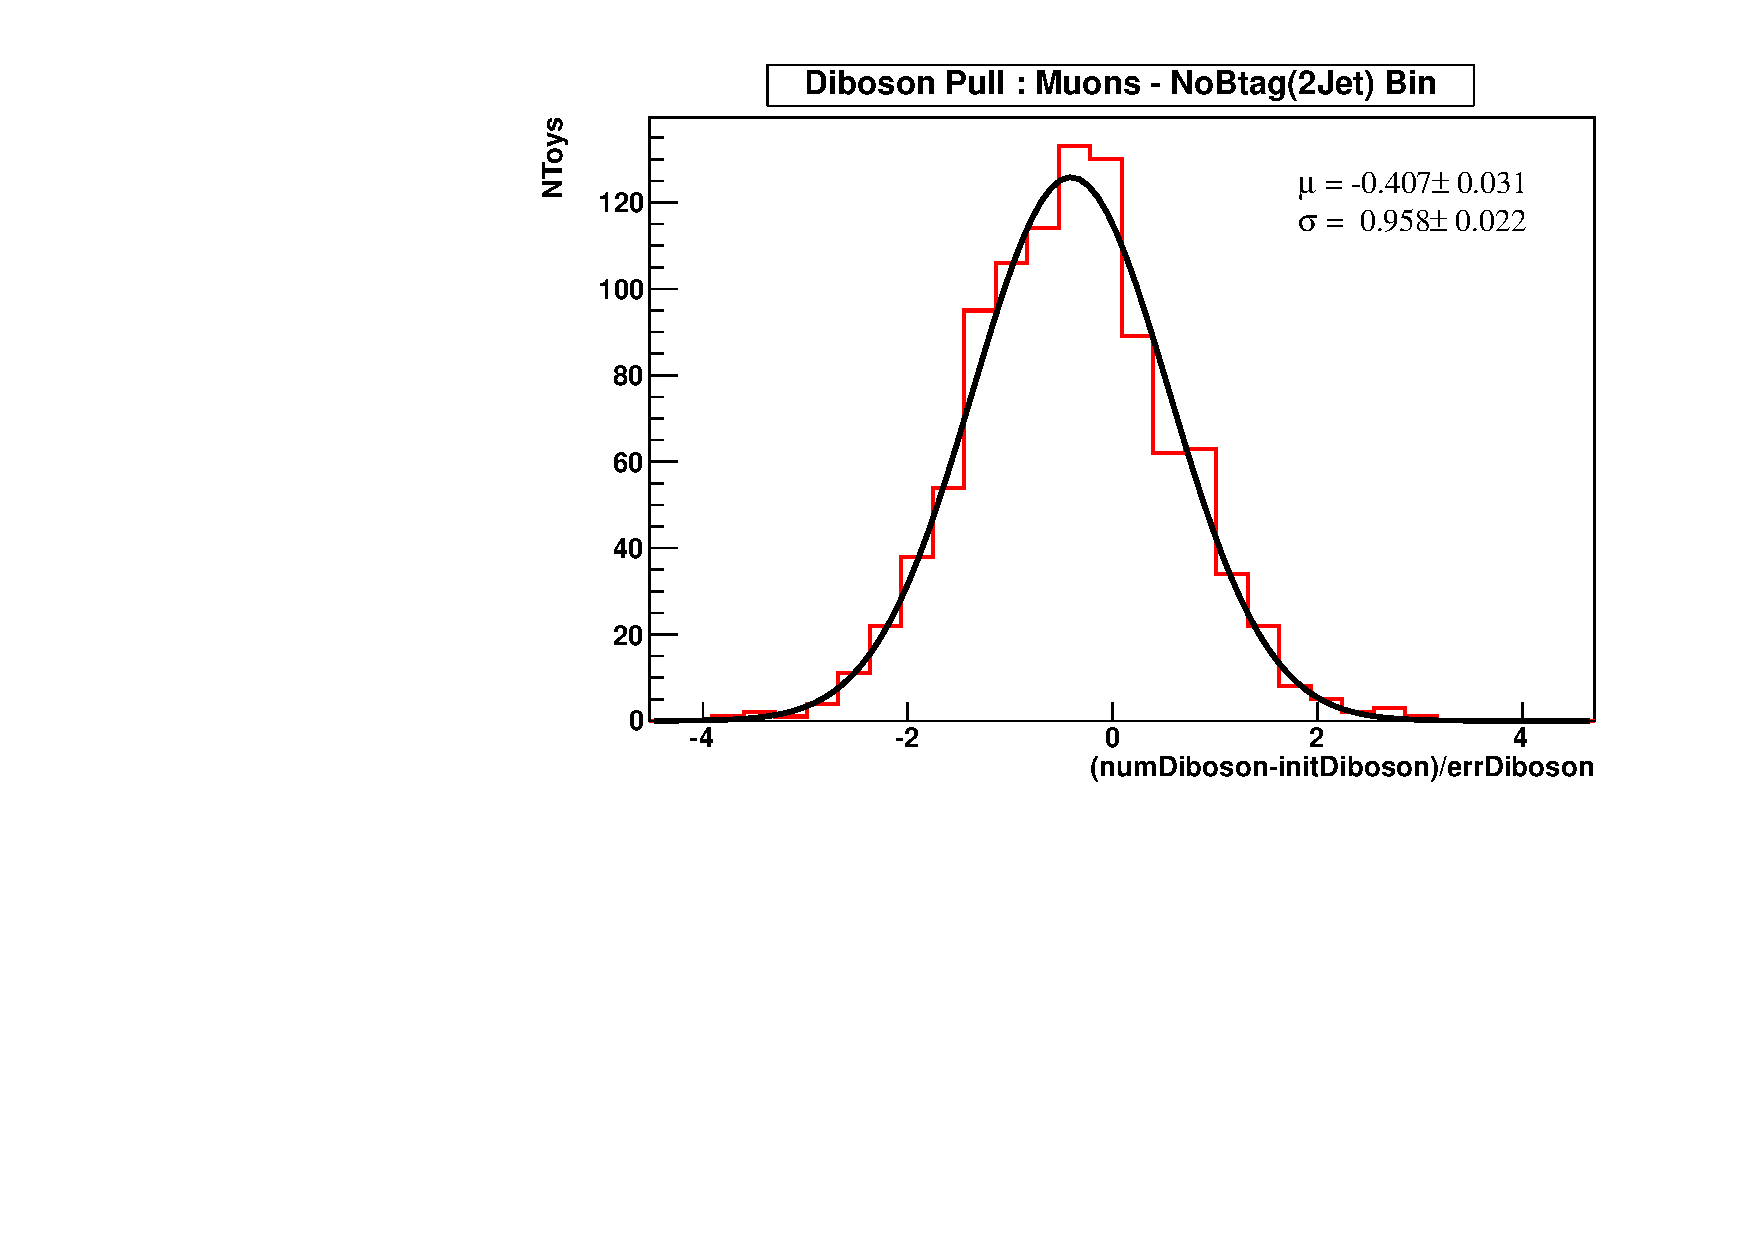
\includegraphics[width=0.96\textwidth]{figs/validation/DibosonPull_Validation_mu_NoBtag_2j.pdf}
\put(-1.5,0.0){(b)} \\
\caption{Fit validation in the untagged (2-jet) bin of the muon channel, using 1000 Toy MC datasets. Diboson (a) Fitted-Given Yield, (b) Pull=(Fitted-Given)/Error.} 
\label{fig:DibosonValidation_mu_NoBTag}}
\end{figure}
%%%%%%%
%%%%%%%
\begin{figure}[h!] {\centering
\unitlength=0.33\linewidth
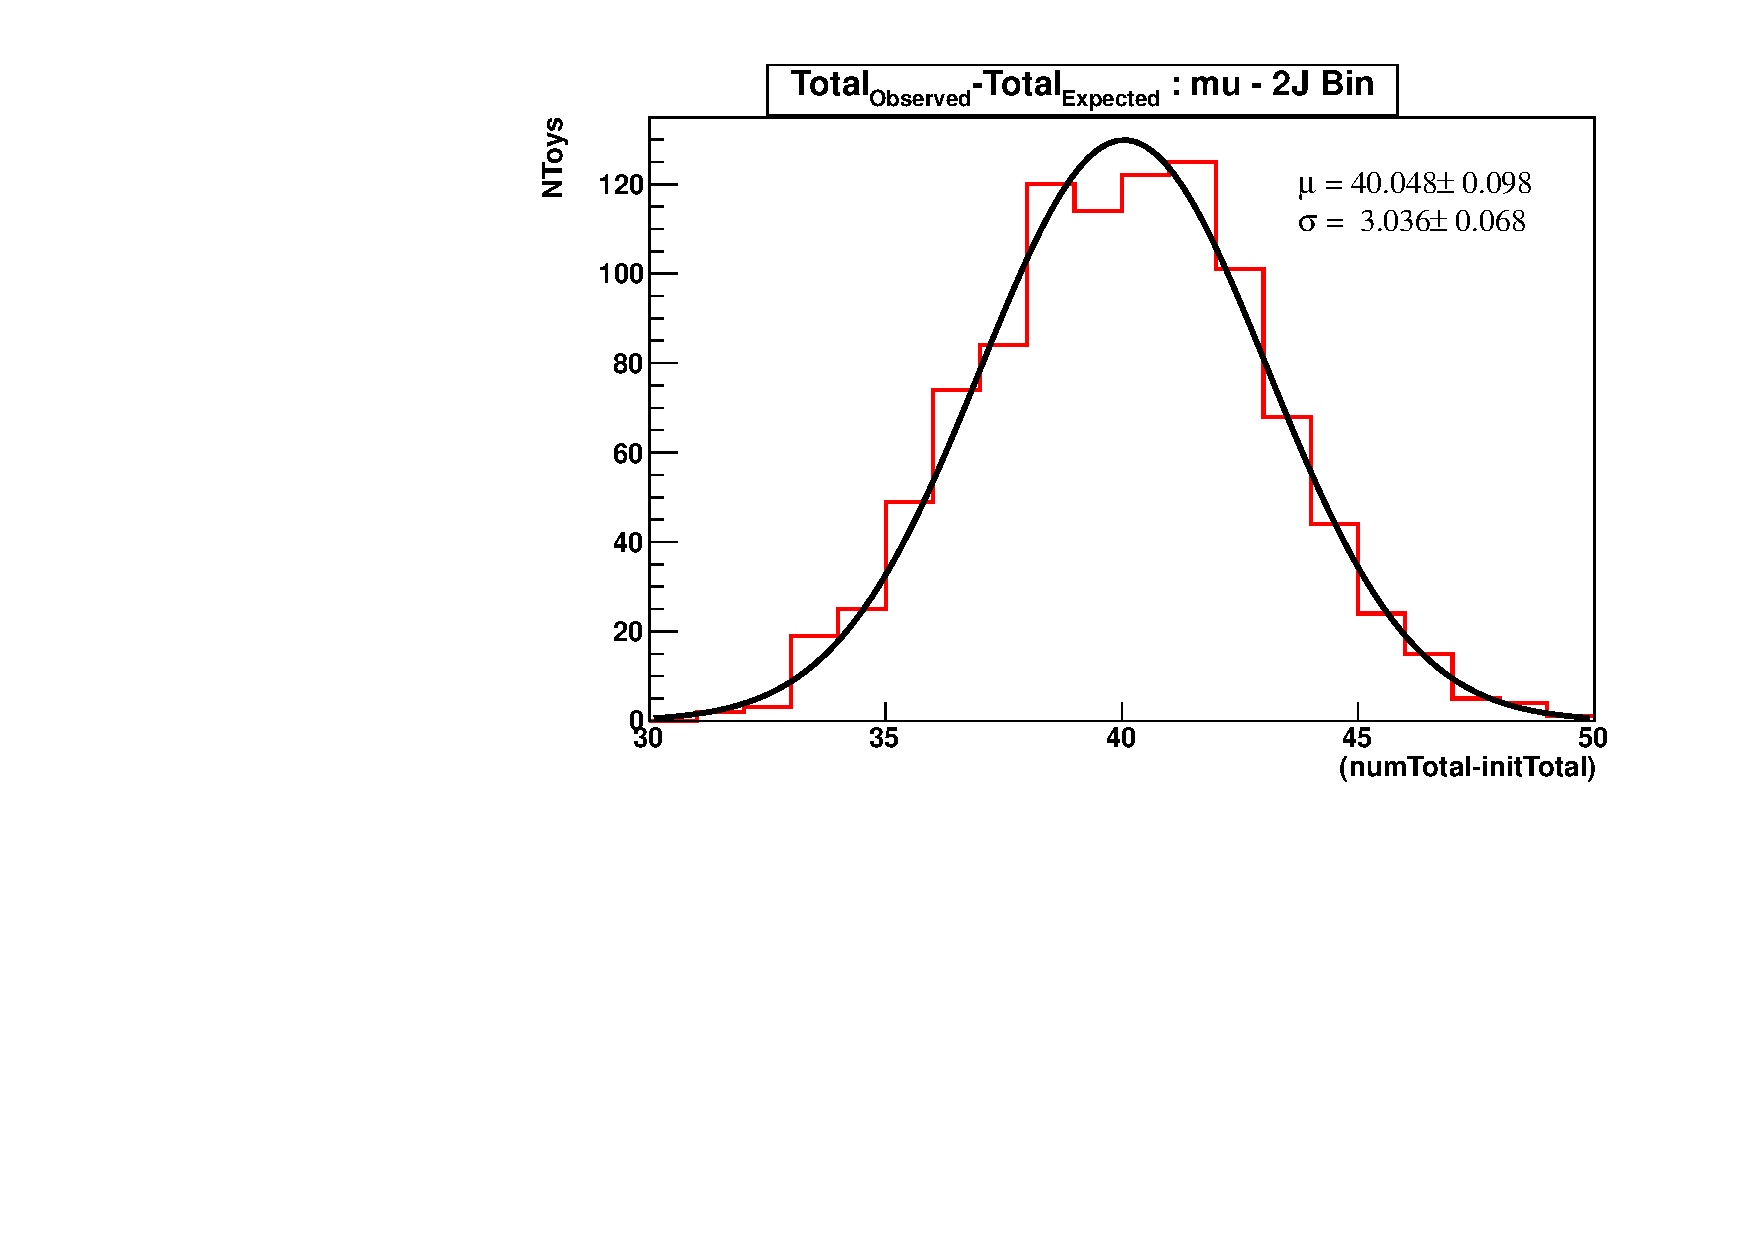
\includegraphics[width=0.48\textwidth]{figs/validation/TotalYield_Validation_mu_NoBtag_2j.pdf}
\put(-0.80,0.0){(a)}\\ 
\unitlength=0.33\linewidth
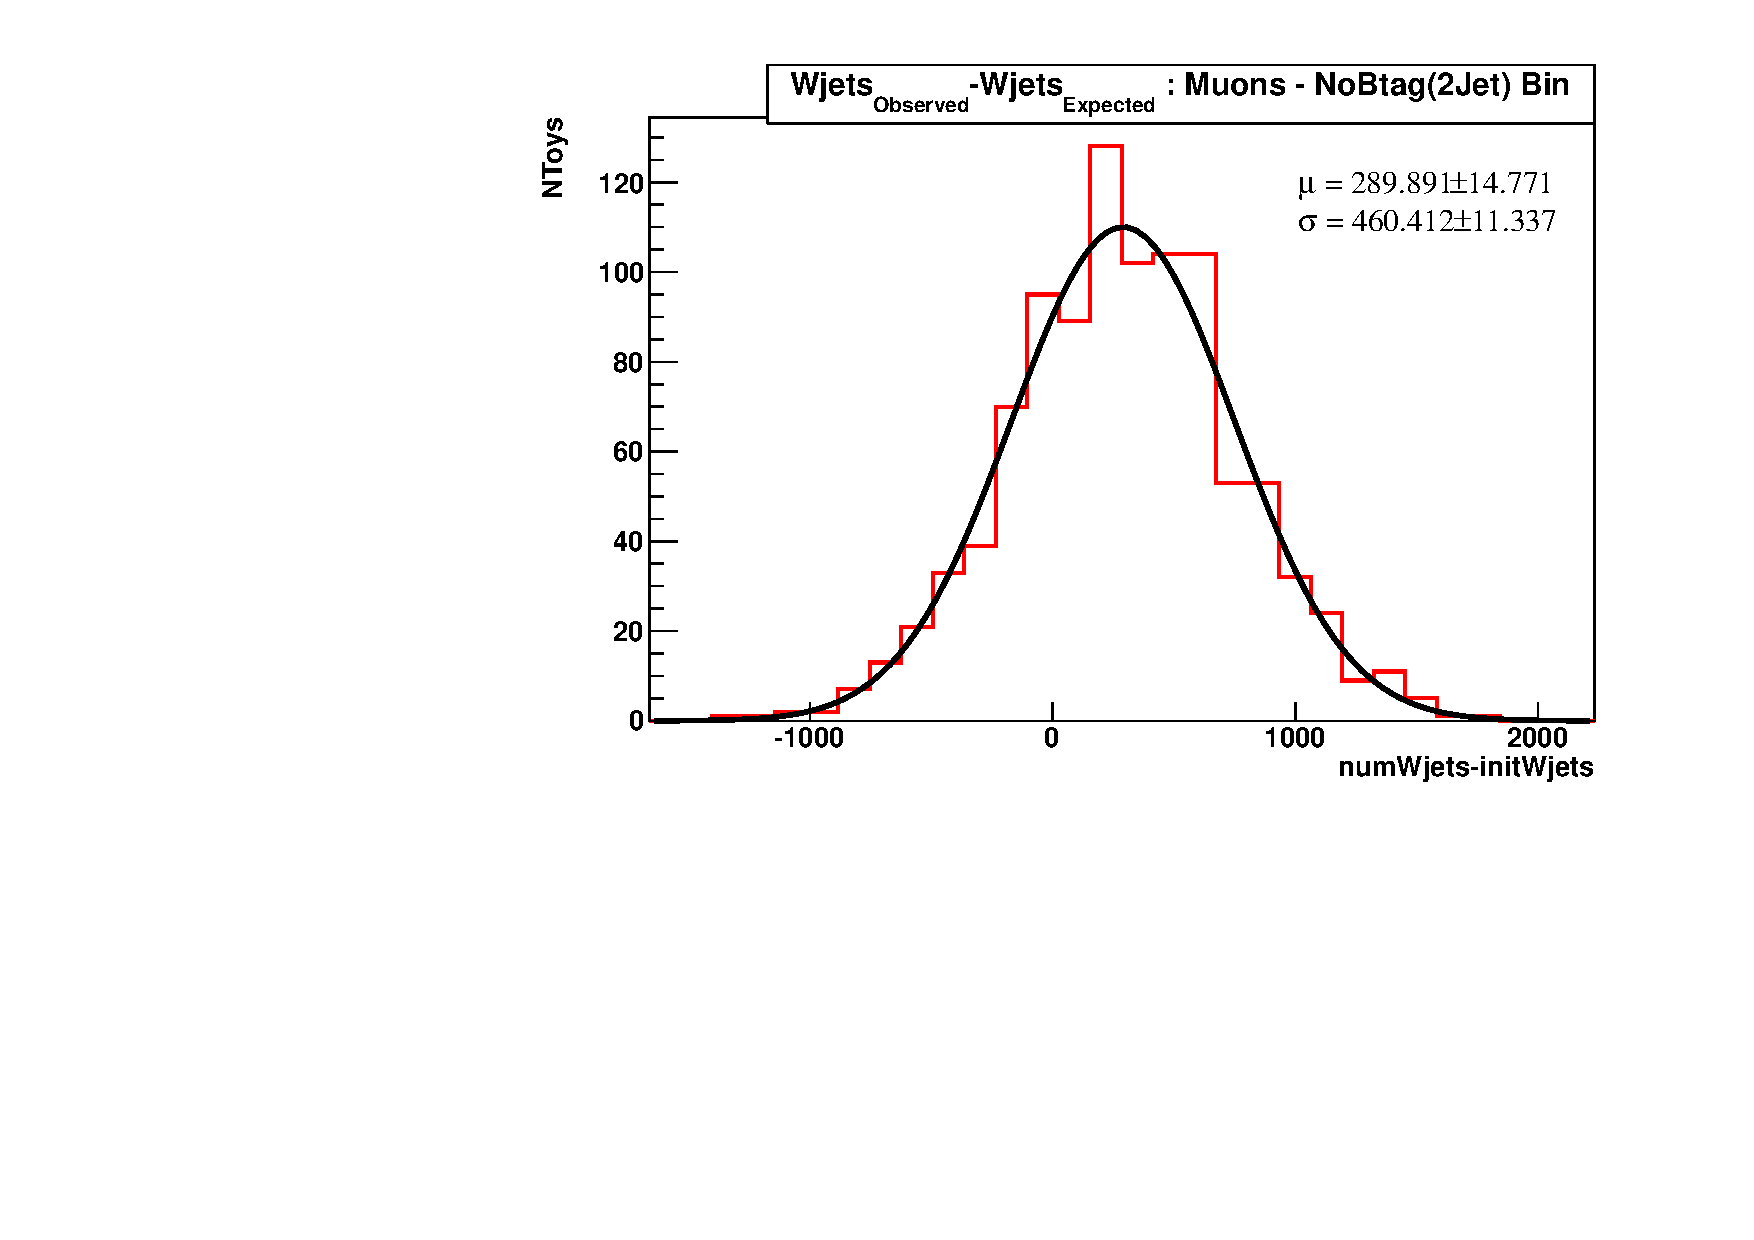
\includegraphics[width=0.48\textwidth]{figs/validation/WjetsYield_Validation_mu_NoBtag_2j.pdf}
\put(-0.80,0.0){(b)} 
\unitlength=0.33\linewidth
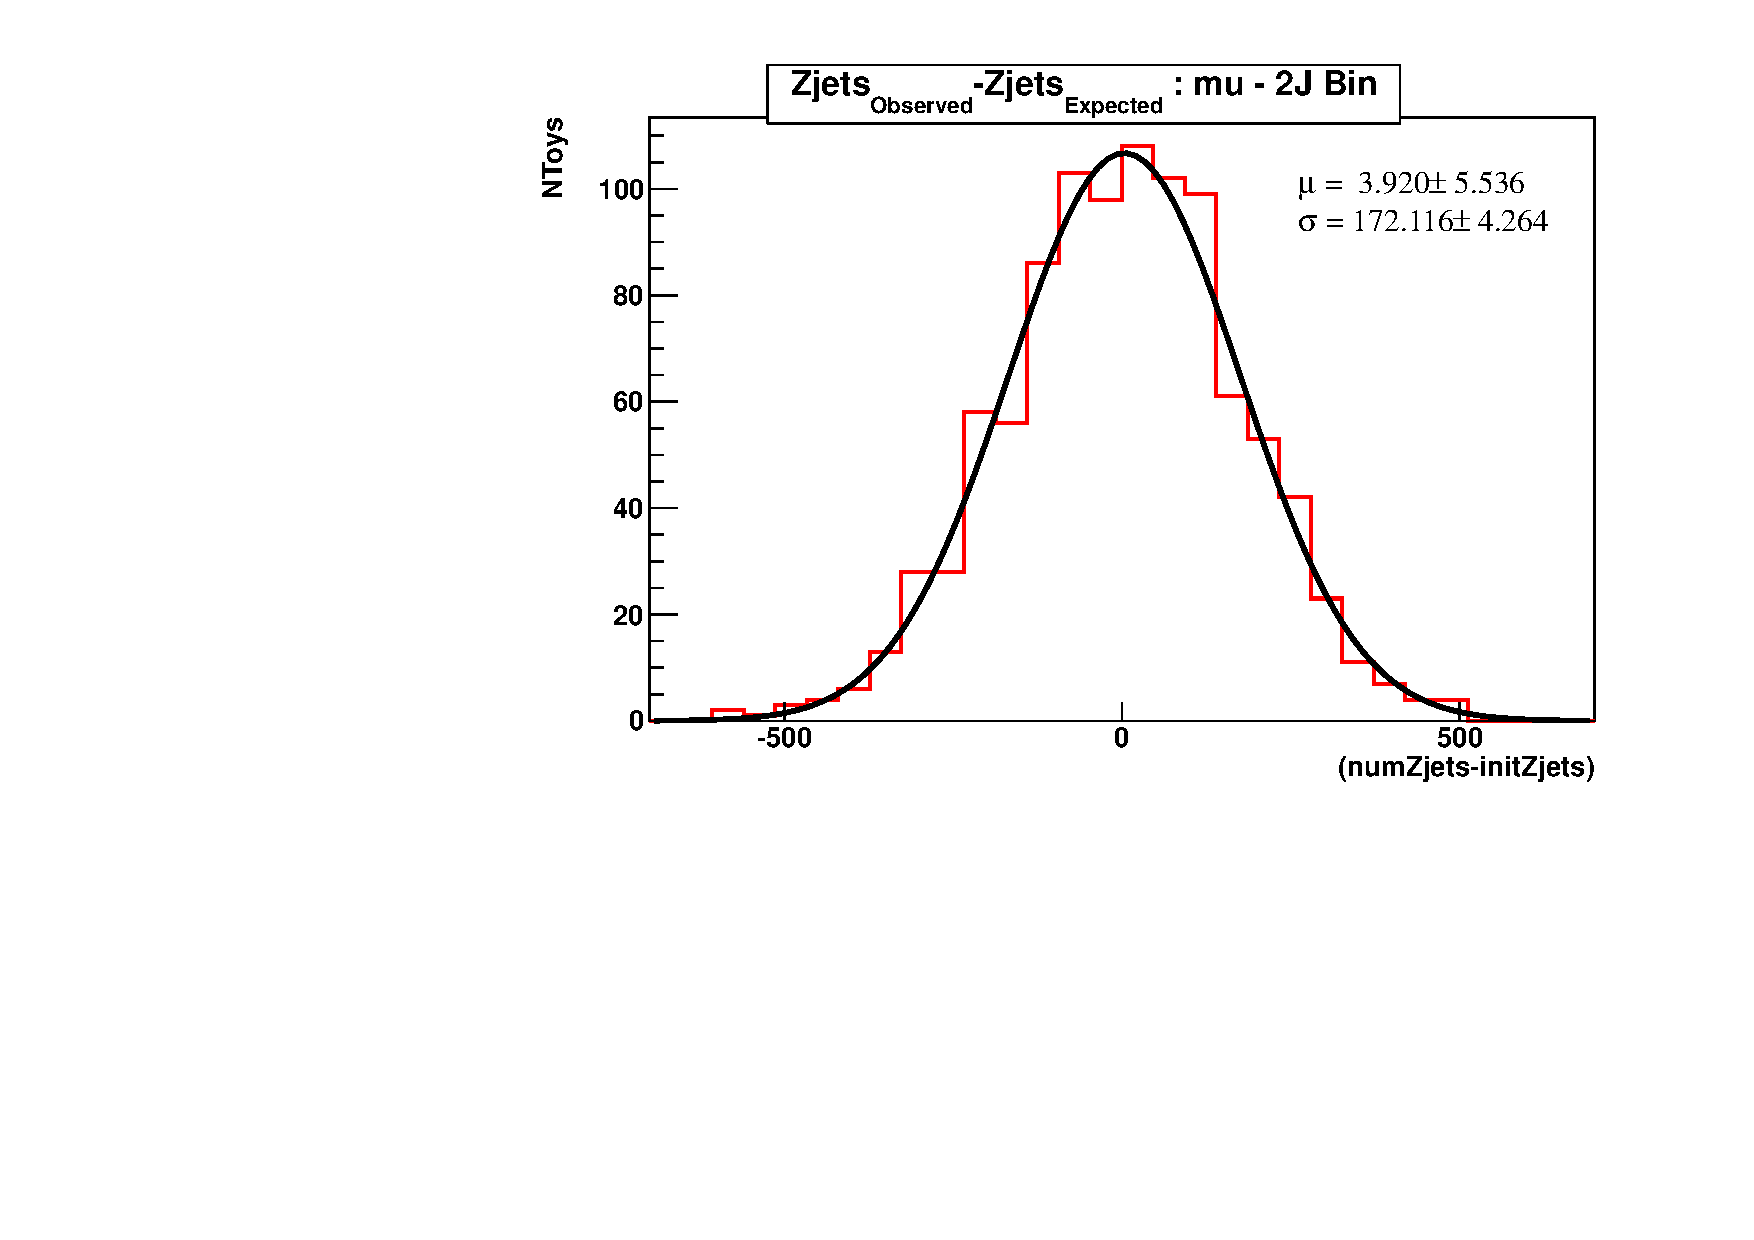
\includegraphics[width=0.48\textwidth]{figs/validation/ZjetsYield_Validation_mu_NoBtag_2j.pdf}
\put(-0.80,0.0){(c)}\\
\unitlength=0.33\linewidth
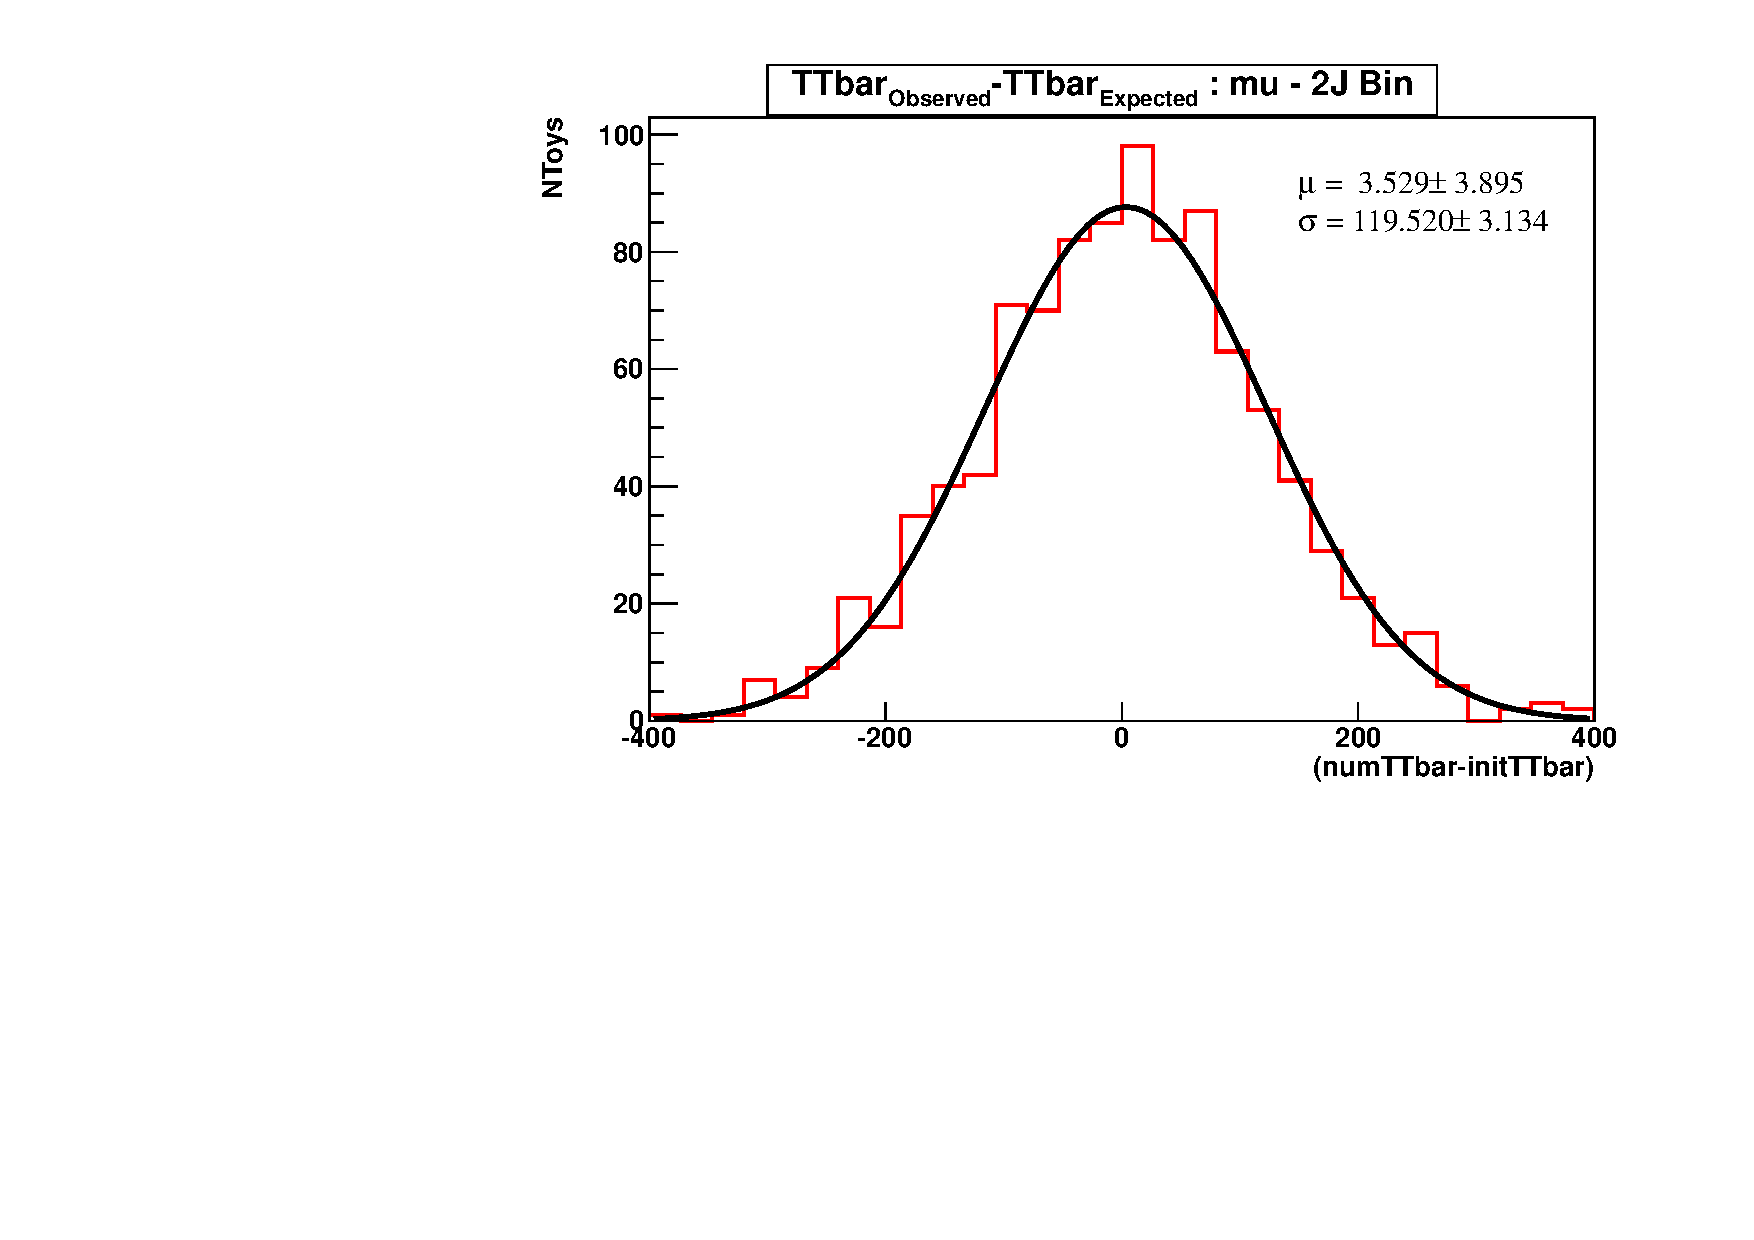
\includegraphics[width=0.48\textwidth]{figs/validation/TTbarYield_Validation_mu_NoBtag_2j.pdf}
\put(-0.80,0.0){(d)} 
\unitlength=0.33\linewidth
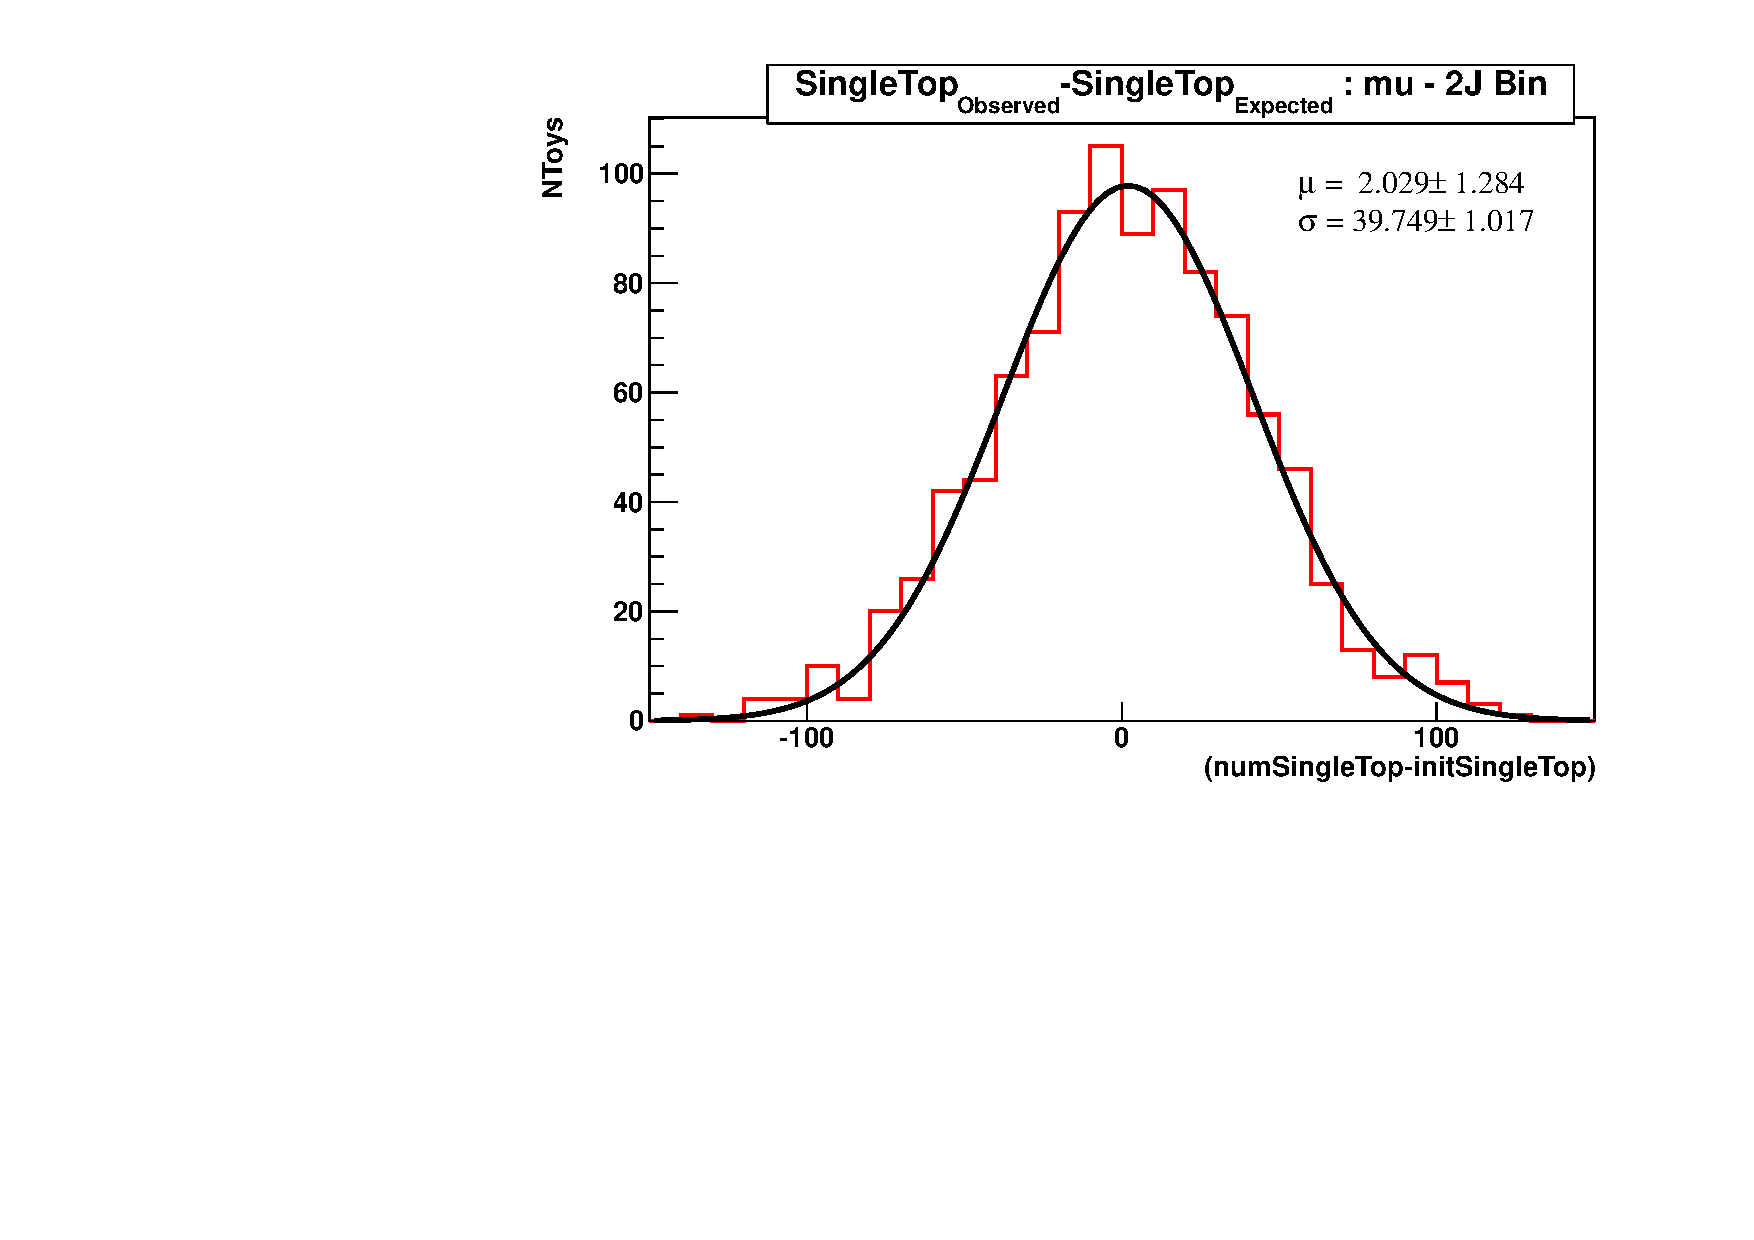
\includegraphics[width=0.48\textwidth]{figs/validation/SingleTopYield_Validation_mu_NoBtag_2j.pdf}
\put(-0.80,0.0){(e)} 
\caption{Fit validation in the  untagged (2-jet) bin of the muon channel, using 1000 Toy MC datasets. Fitted-Given yields for: (a) Total, (b) W+jets, (c) Z+jets, (d) $t\bar{t}$, (e) SingleTop.} 
\label{fig:Validation_Yields_mu_NoBTag_2j}}
\end{figure}
%%%%%%%
%%%%%%%
\begin{figure}[h!] {\centering
\unitlength=0.33\linewidth
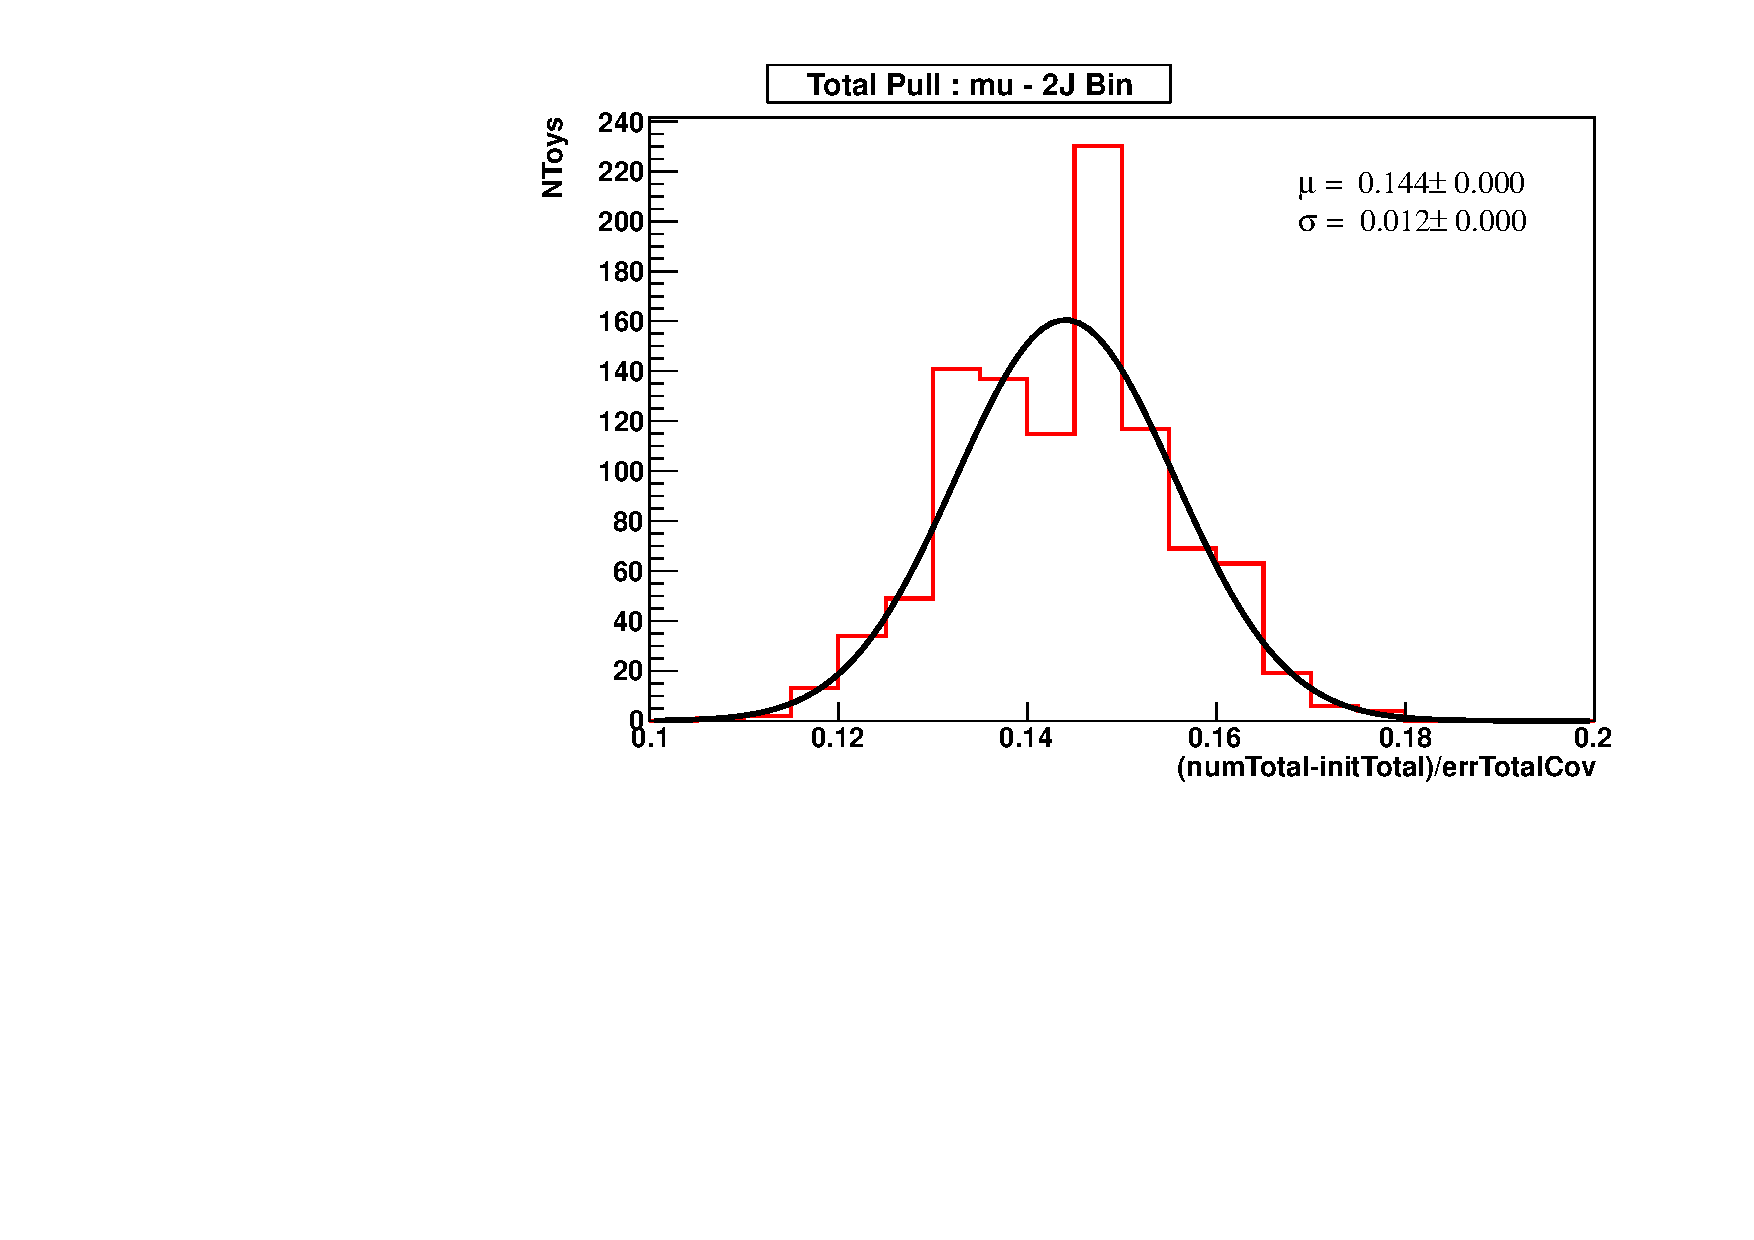
\includegraphics[width=0.48\textwidth]{figs/validation/TotalPull_Validation_mu_NoBtag_2j.pdf}
\put(-0.80,0.0){(a)}\\ 
\unitlength=0.33\linewidth
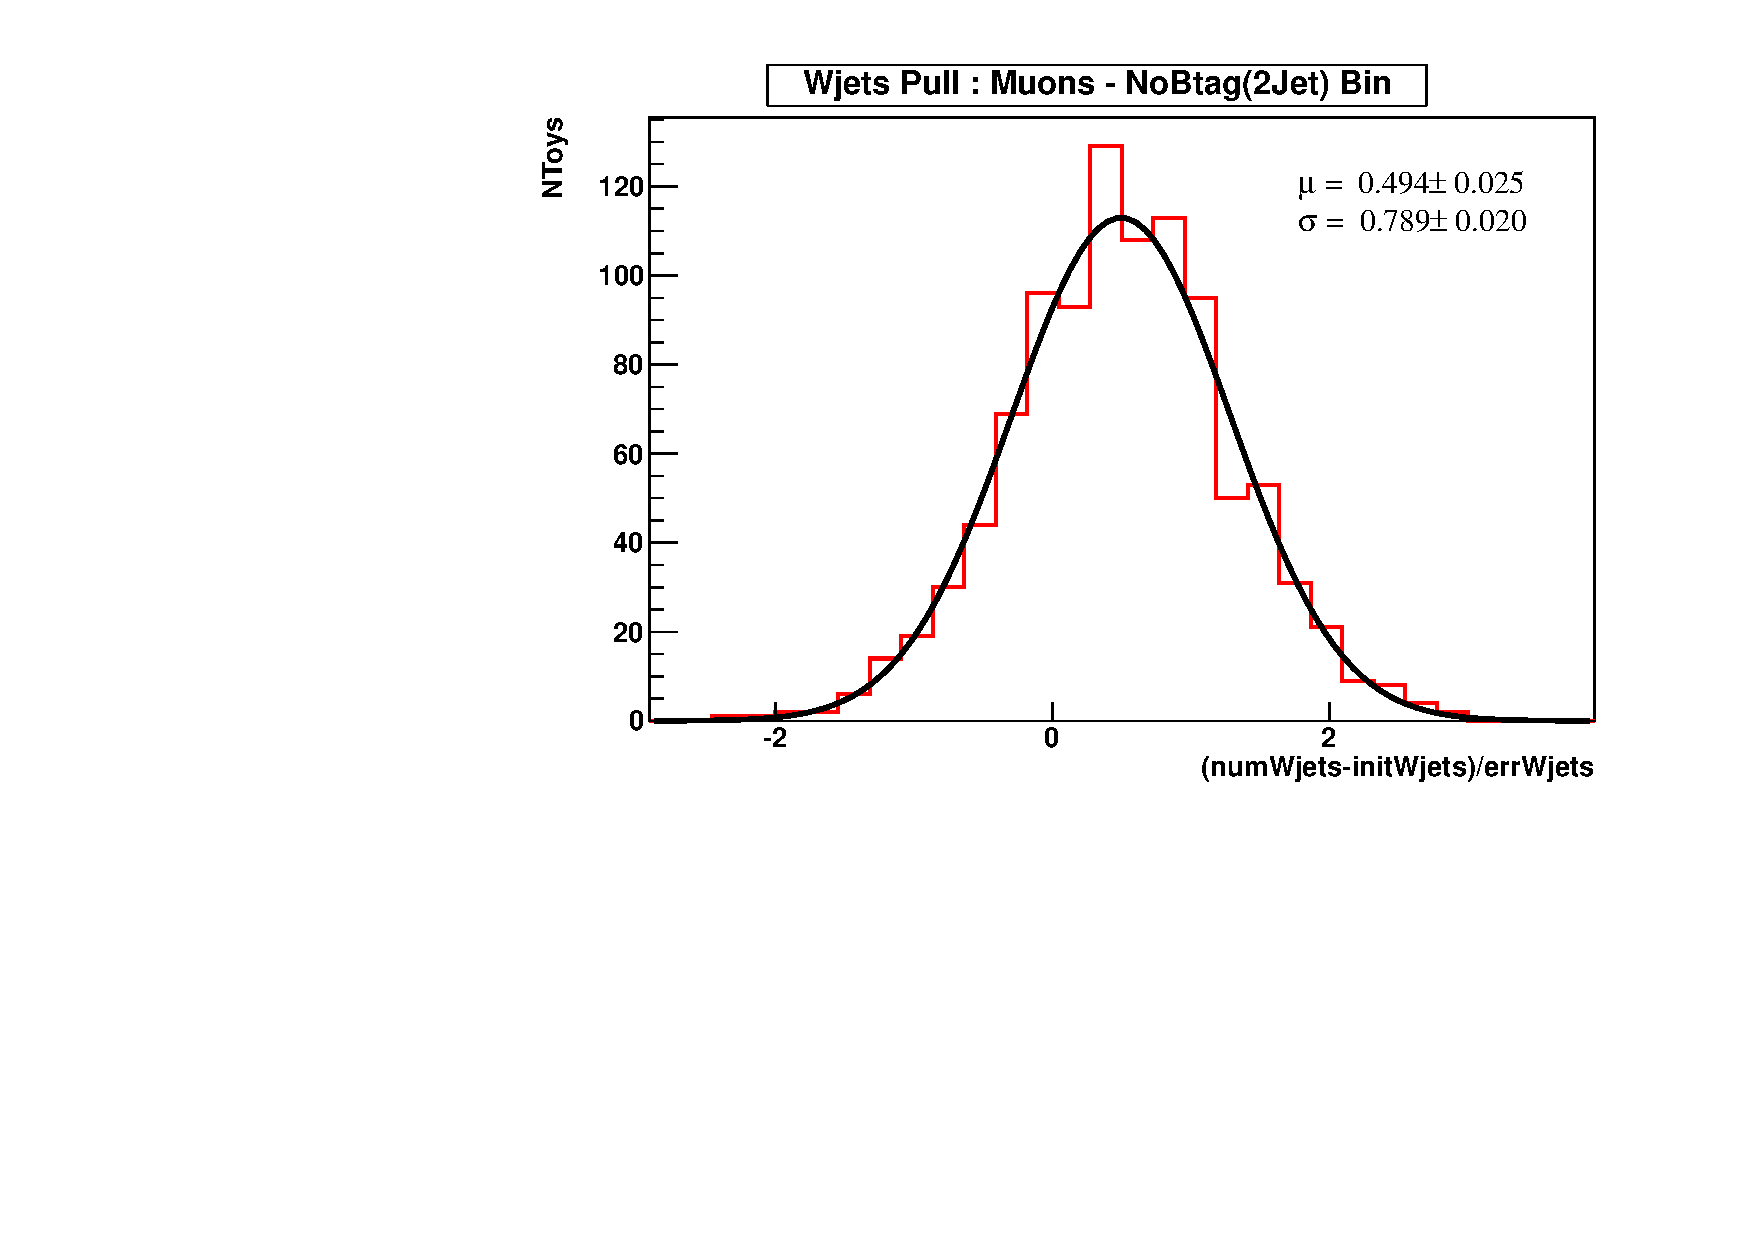
\includegraphics[width=0.48\textwidth]{figs/validation/WjetsPull_Validation_mu_NoBtag_2j.pdf}
\put(-0.80,0.0){(b)}
\unitlength=0.33\linewidth
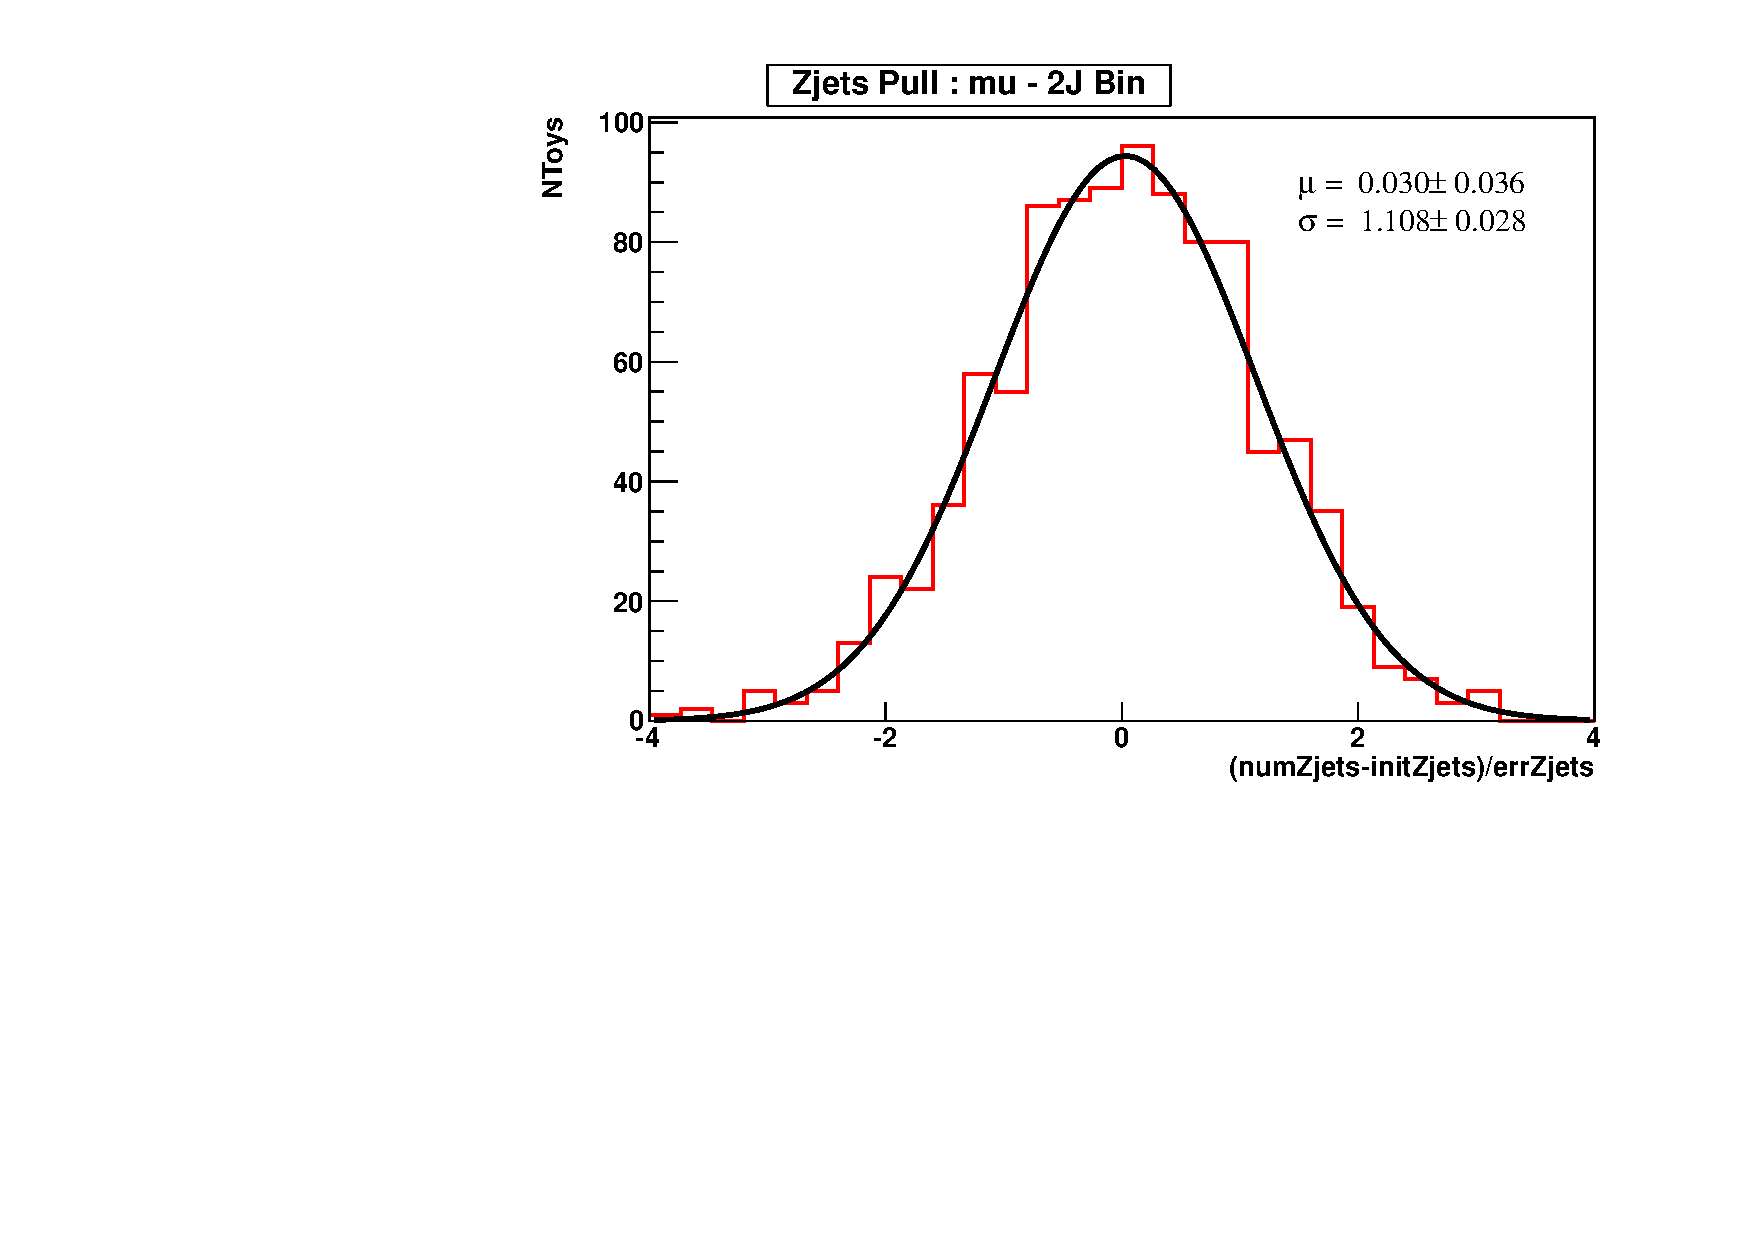
\includegraphics[width=0.48\textwidth]{figs/validation/ZjetsPull_Validation_mu_NoBtag_2j.pdf}
\put(-0.80,0.0){(c)}\\
\unitlength=0.33\linewidth
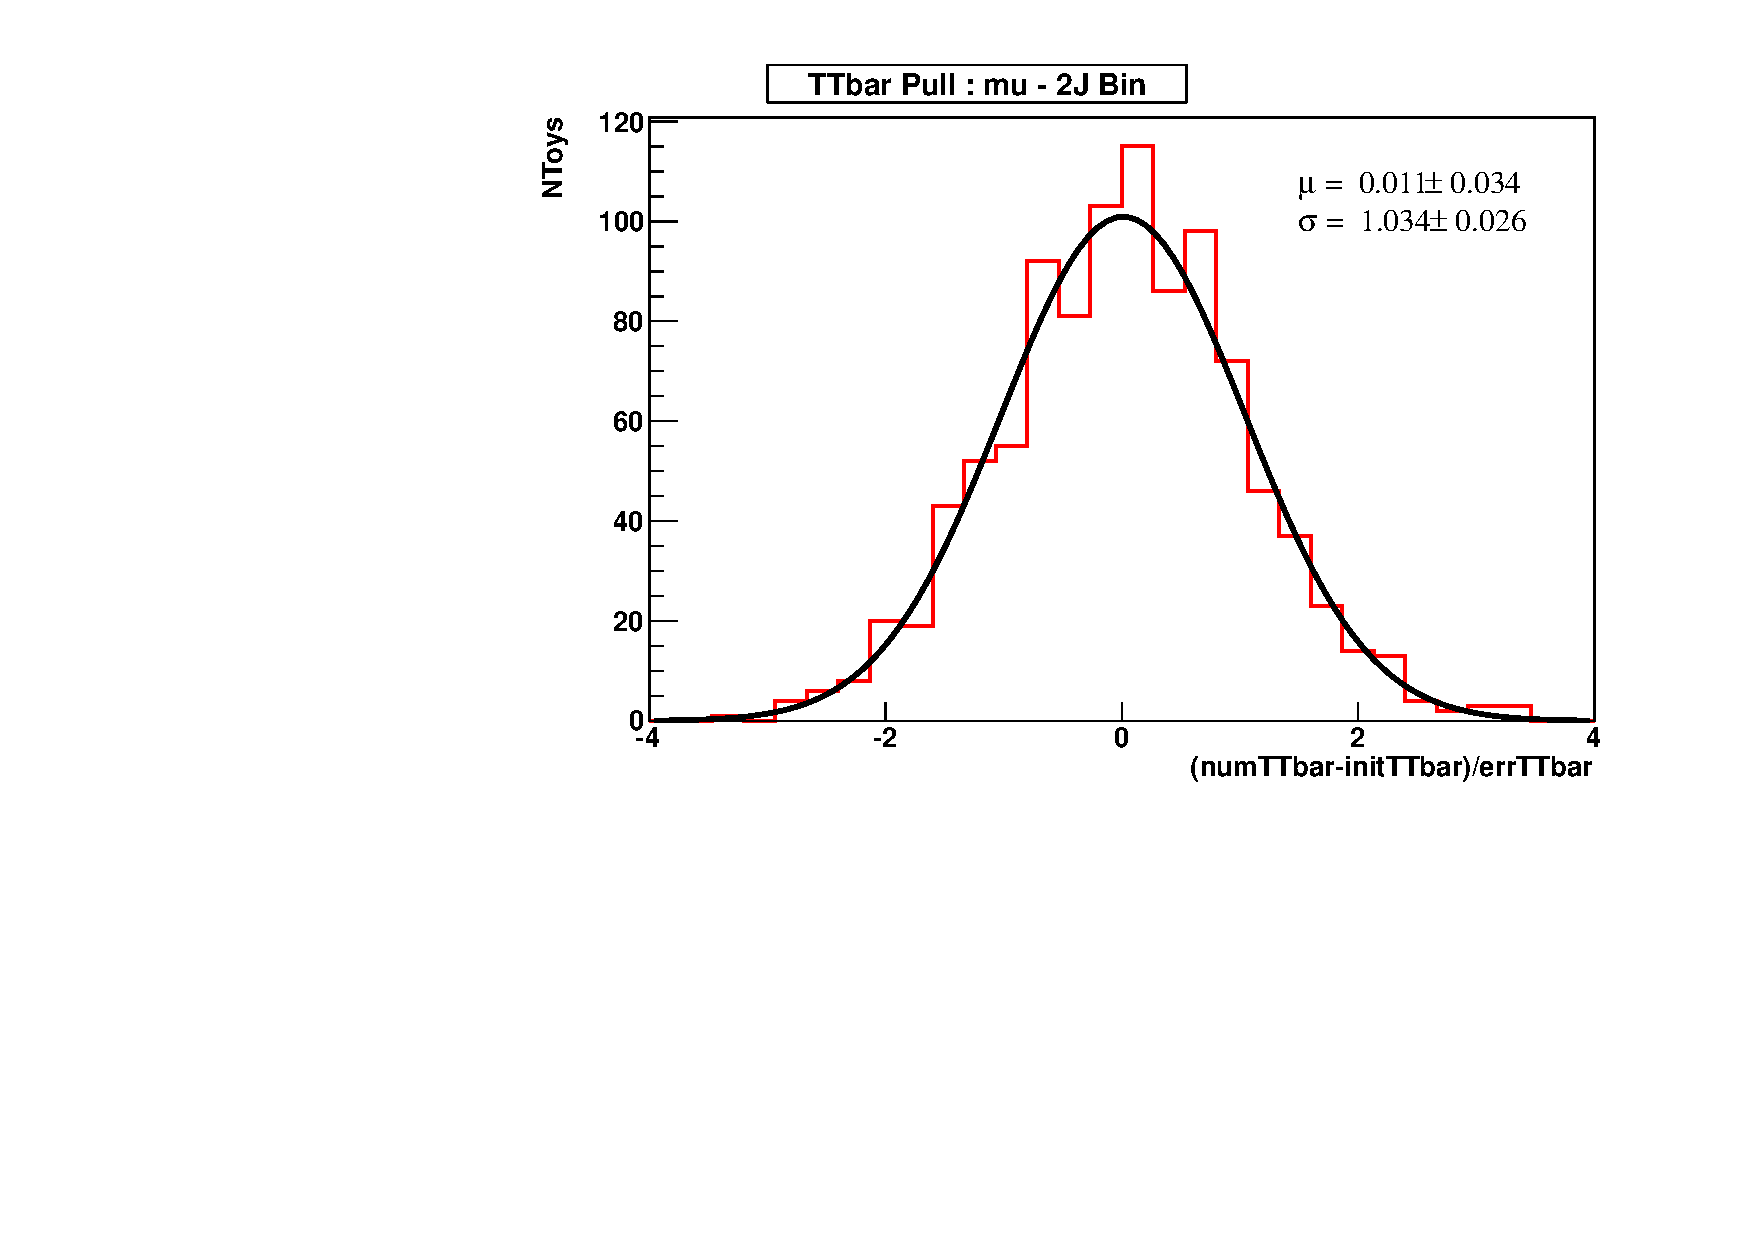
\includegraphics[width=0.48\textwidth]{figs/validation/TTbarPull_Validation_mu_NoBtag_2j.pdf}
\put(-0.80,0.0){(d)} 
\unitlength=0.33\linewidth
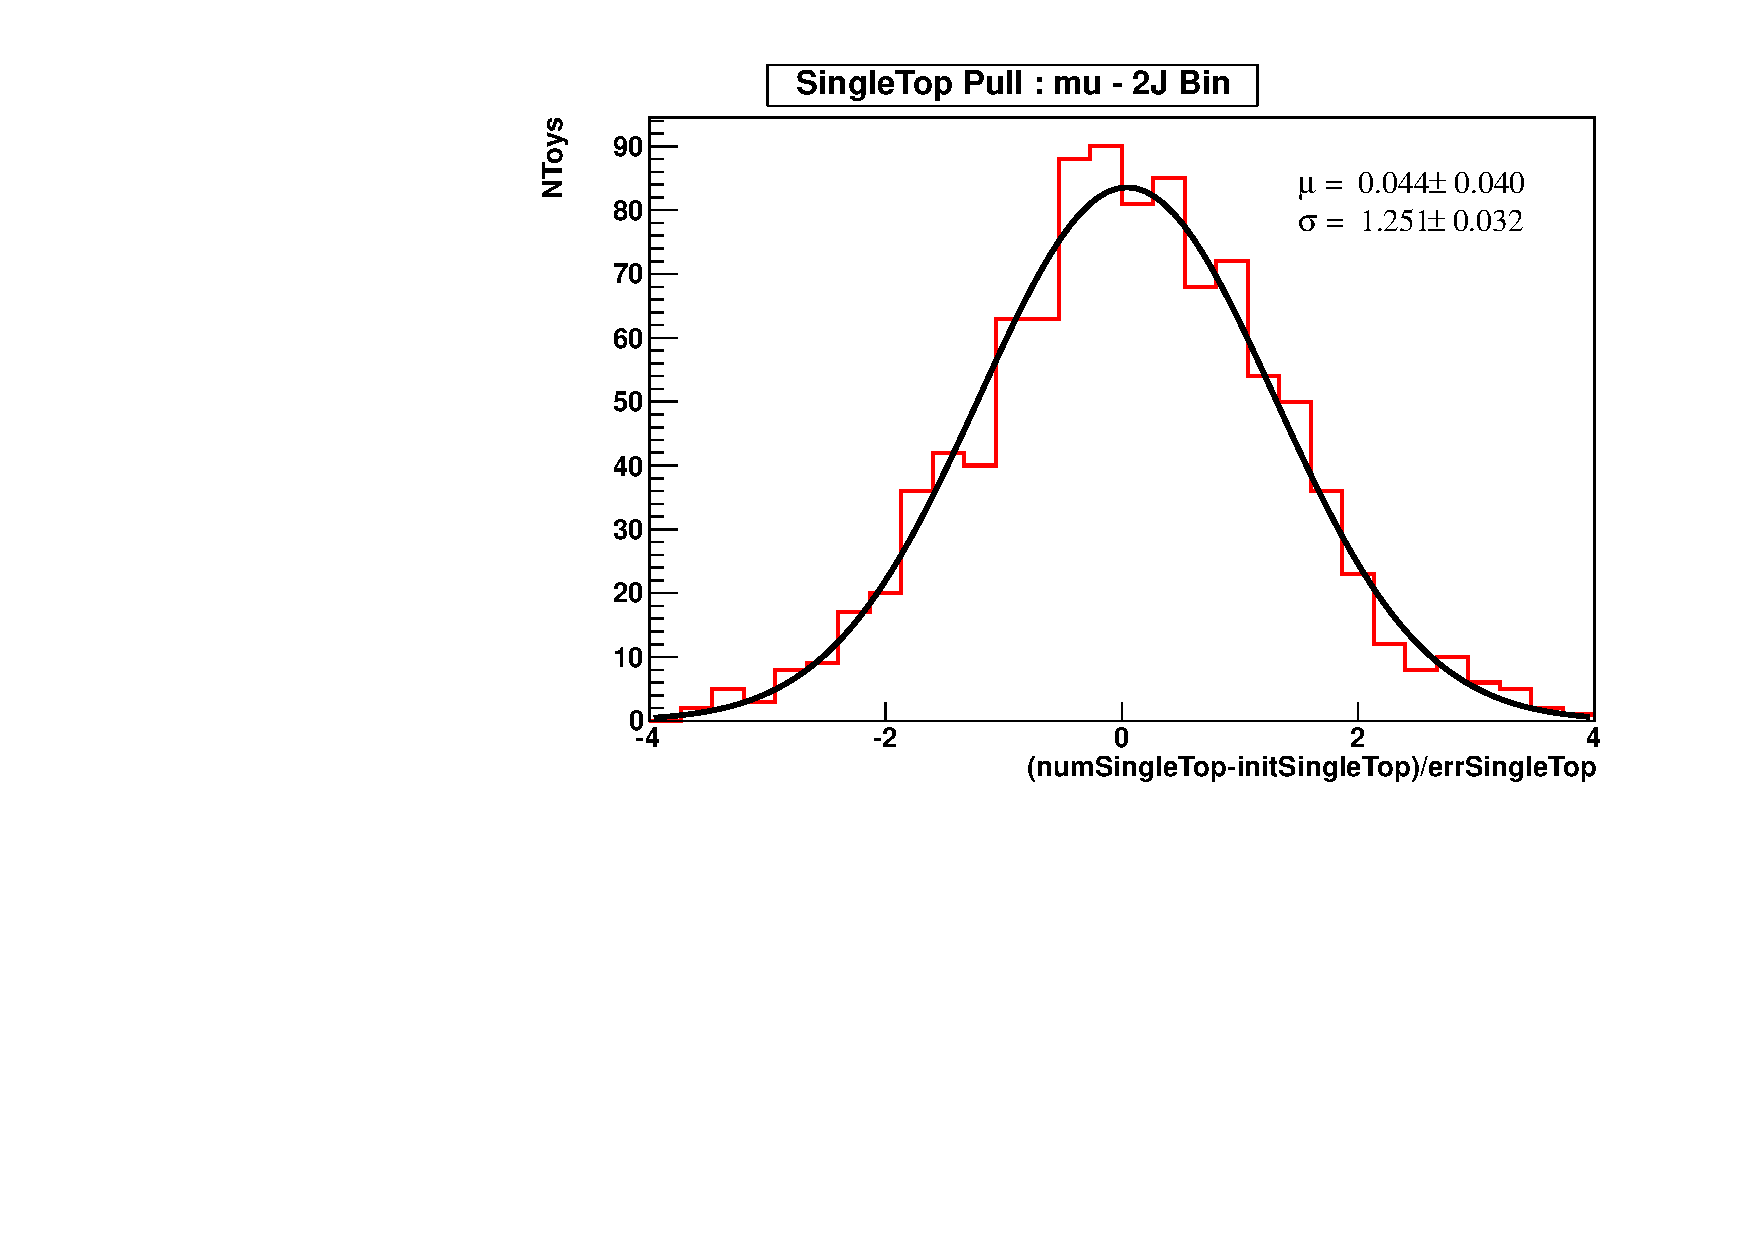
\includegraphics[width=0.48\textwidth]{figs/validation/SingleTopPull_Validation_mu_NoBtag_2j.pdf}
\put(-0.80,0.0){(e)} 
\caption{Fit validation in the  untagged (2-jet) bin of the muon channel, using 1000 Toy MC datasets. Pull=(Fitted-Given)/Error for: (a) Total, (b) W+jets, (c) Z+jets, (d) $t\bar{t}$, (e) SingleTop.} 
\label{fig:Validation_Pulls_mu_NoBTag_2j}}
\end{figure}
%%%%%%%
%%%%%%%
\begin{figure}[h!] {\centering
\unitlength=0.33\linewidth
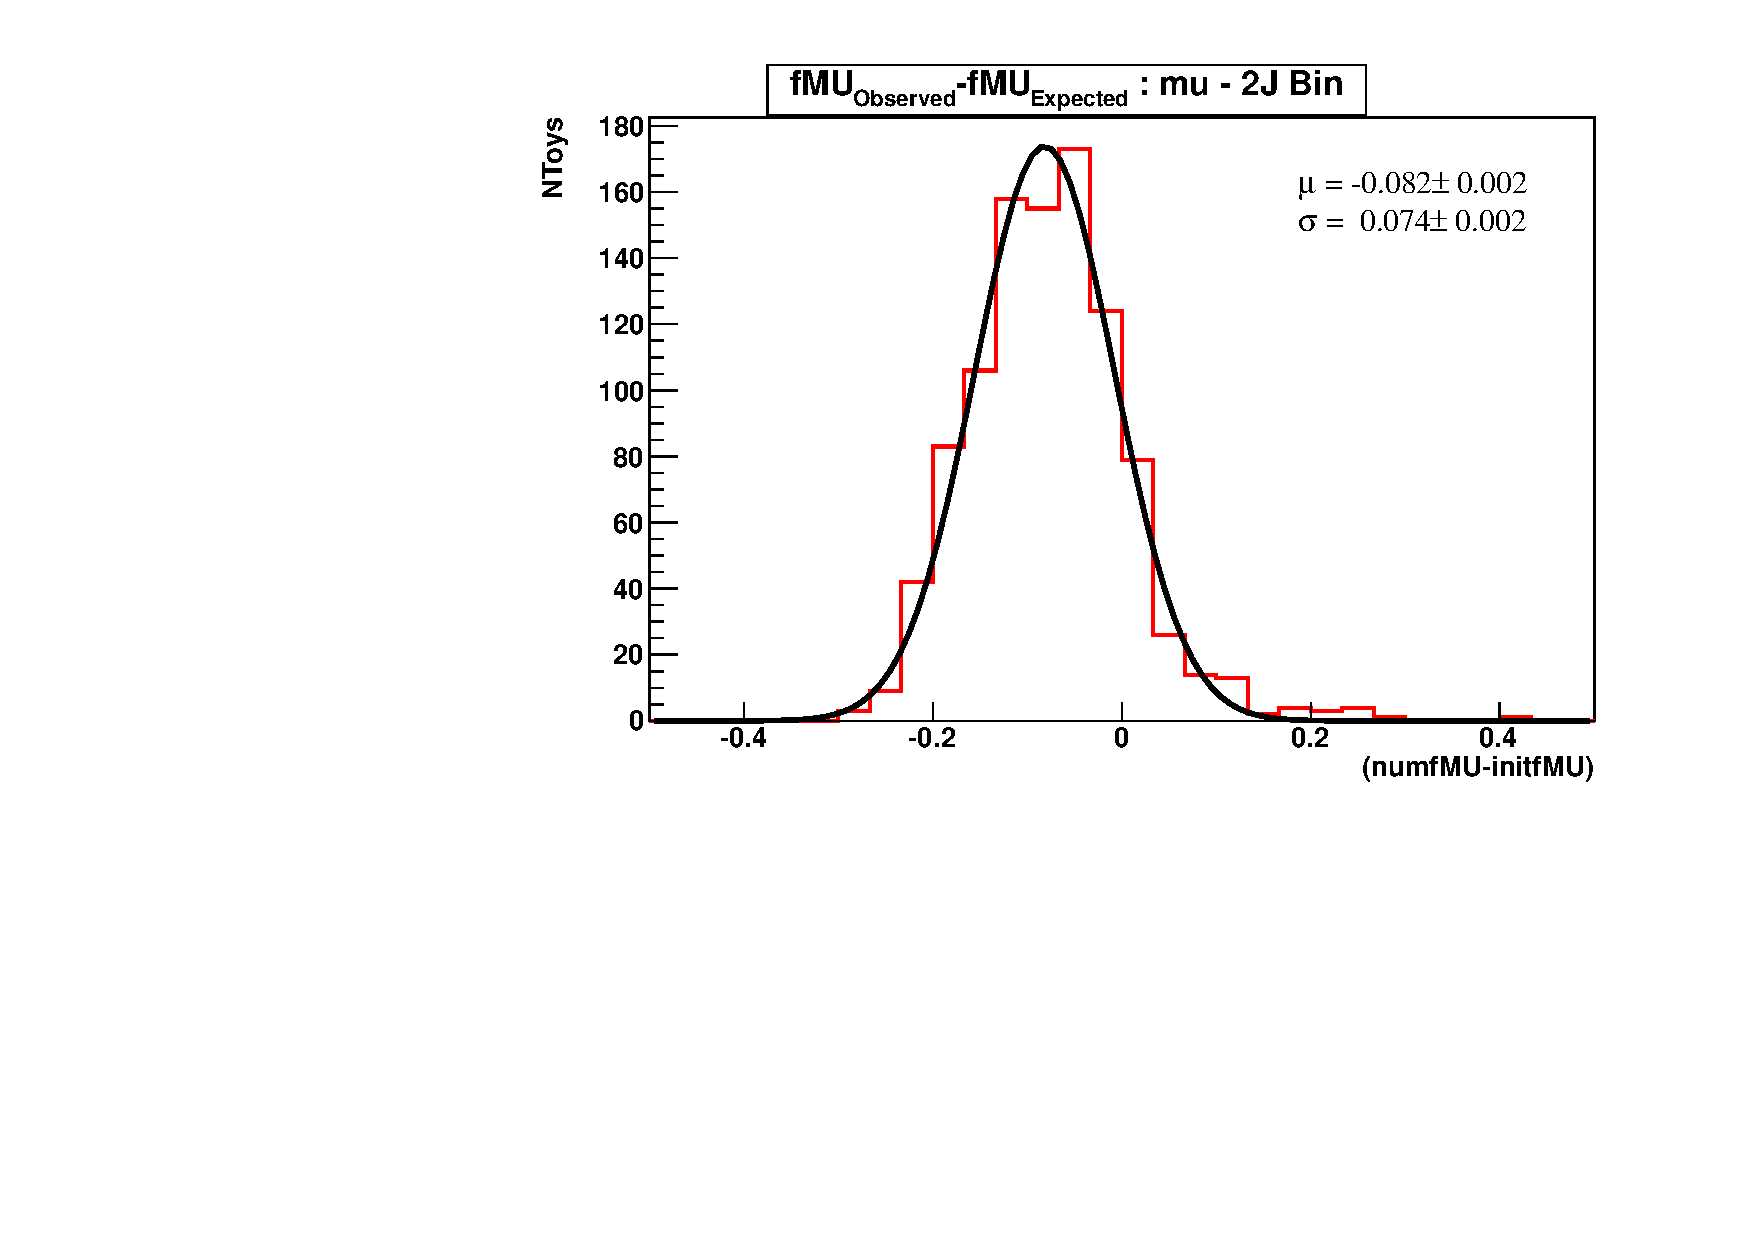
\includegraphics[width=0.48\textwidth]{figs/validation/fMUYield_Validation_mu_NoBtag_2j.pdf}
\put(-0.80,0.0){(a)} 
\unitlength=0.33\linewidth
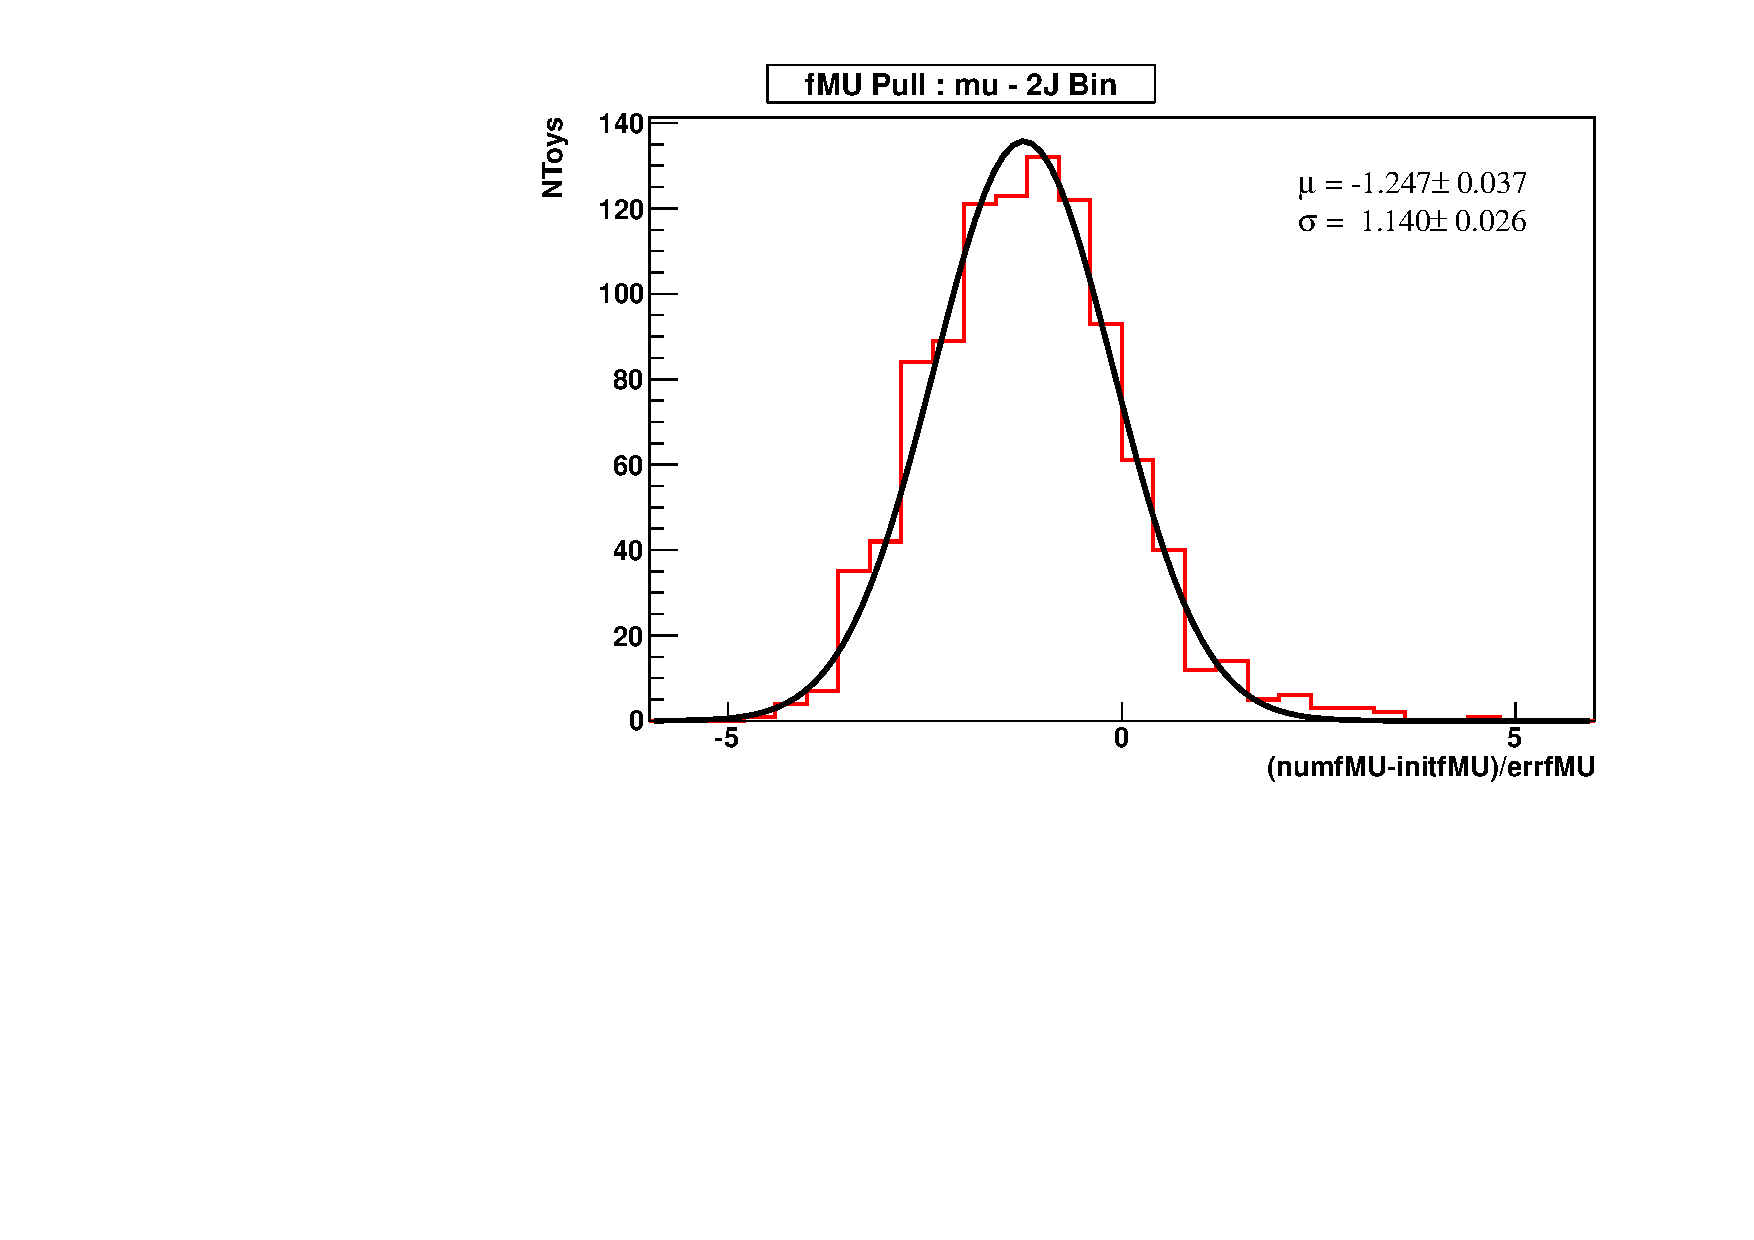
\includegraphics[width=0.48\textwidth]{figs/validation/fMUPull_Validation_mu_NoBtag_2j.pdf}
\put(-0.80,0.0){(b)} \\
\unitlength=0.33\linewidth
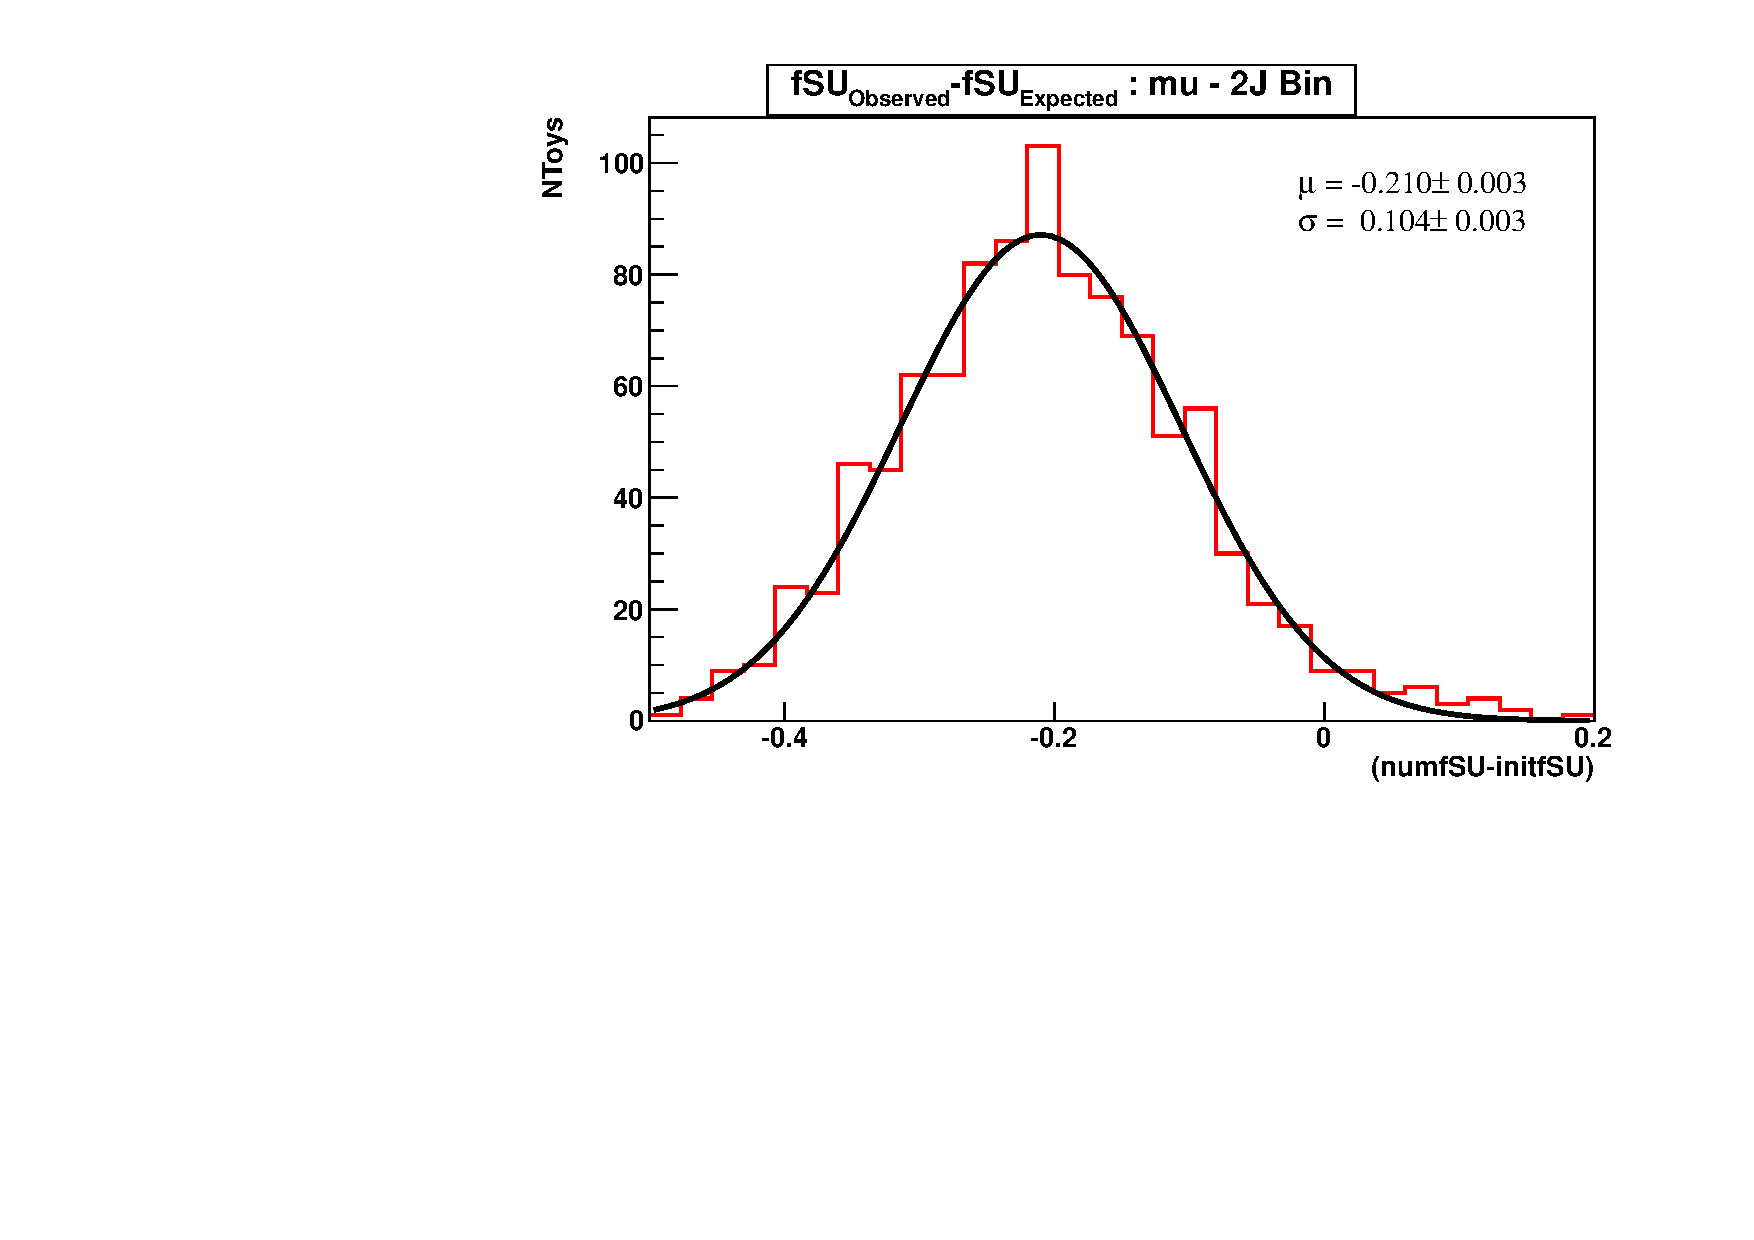
\includegraphics[width=0.48\textwidth]{figs/validation/fSUYield_Validation_mu_NoBtag_2j.pdf}
\put(-0.80,0.0){(c)} 
\unitlength=0.33\linewidth
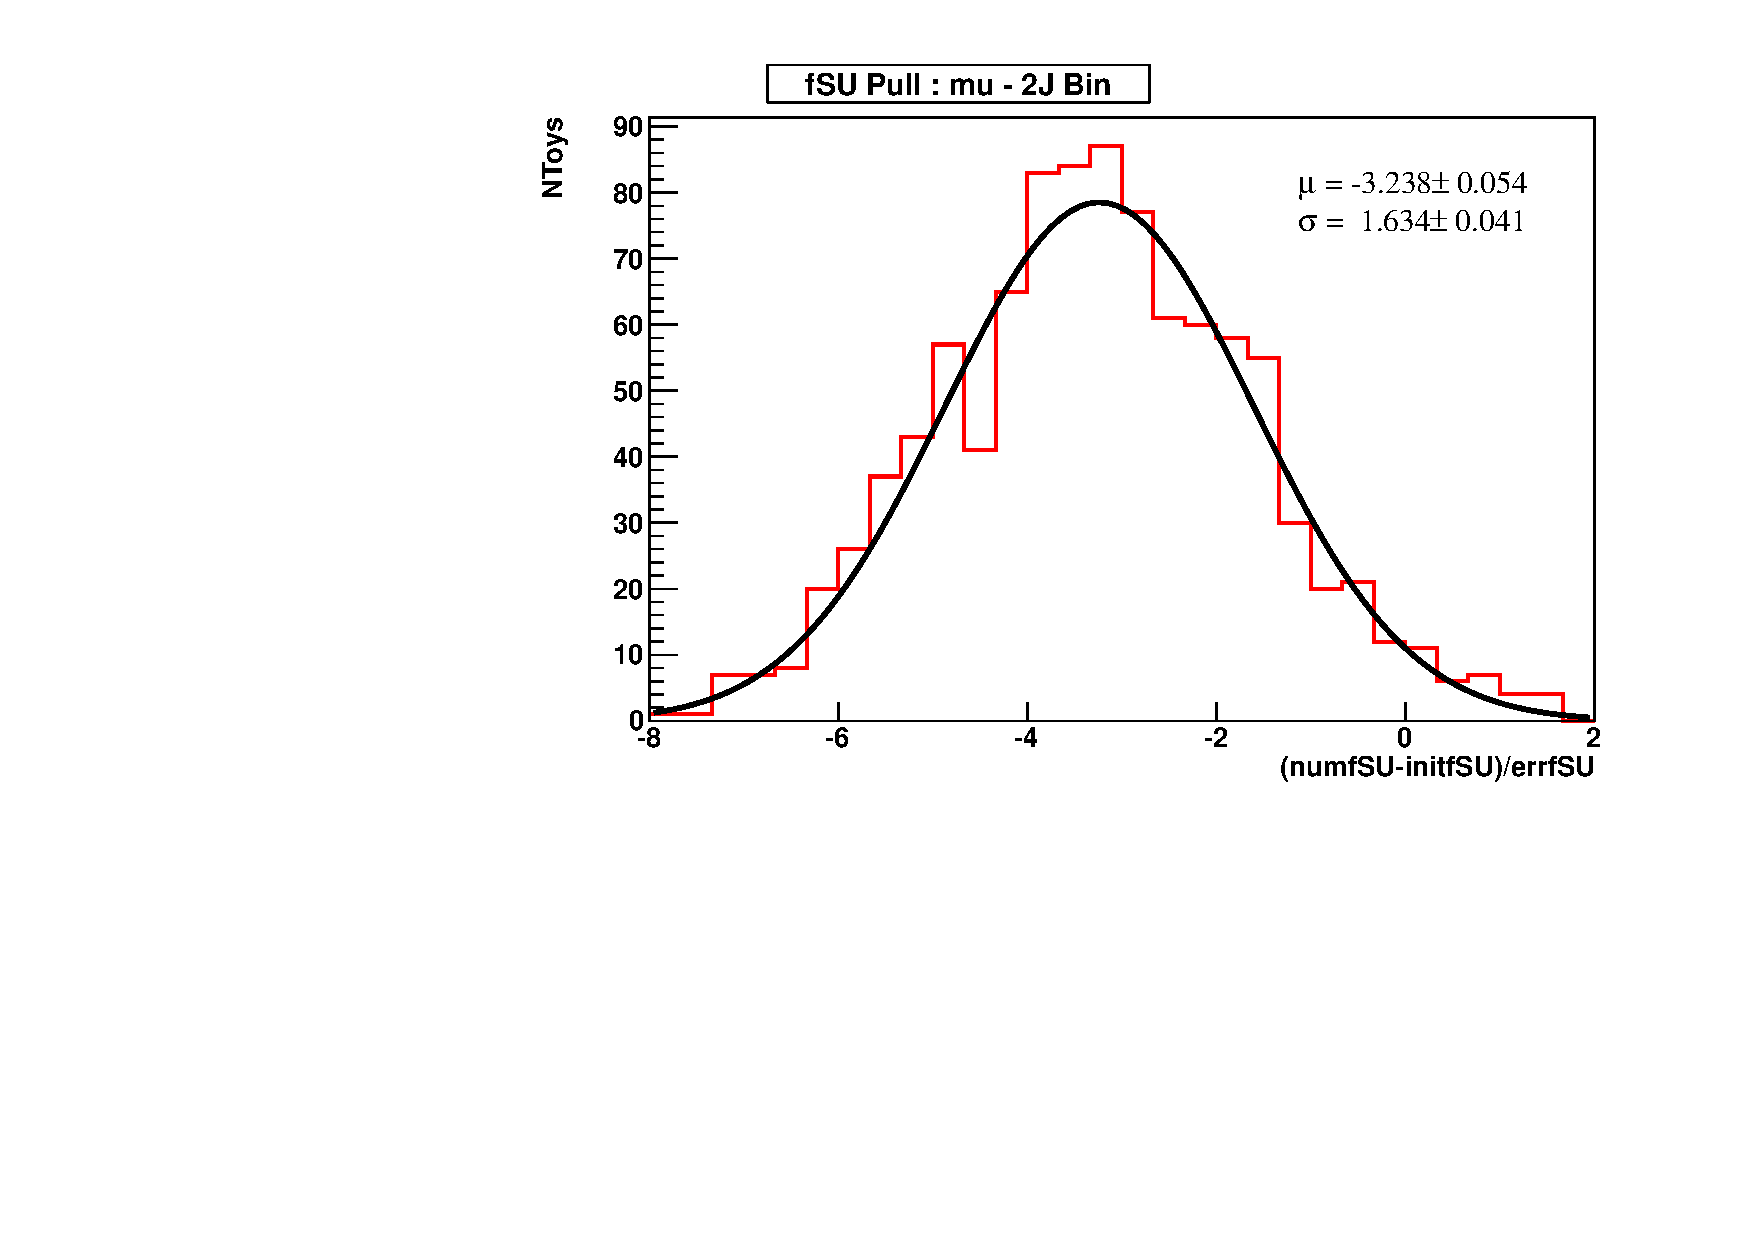
\includegraphics[width=0.48\textwidth]{figs/validation/fSUPull_Validation_mu_NoBtag_2j.pdf}
\put(-0.80,0.0){(d)}
\caption{Fit validation in the untagged (2-jet) bin of the muon channel, using 1000 Toy MC datasets. Matching Up Fraction (a) Fitted-Given (b) Pull distributions; and Scale Up Fraction (c) Fitted-Given (d) Pull distributions. By convention $fMU<0$ ($fSU<0$) denotes that we are using the Matching Down (Scale Down) sample with the fraction $-fMU$ ($-fSU$).} 
\label{fig:Validation_fMUfSU_mu_NoBTag_2j}}
\end{figure}
%%%%%%%
%%%%%%%
\begin{figure}[h!] {\centering
\unitlength=0.33\linewidth
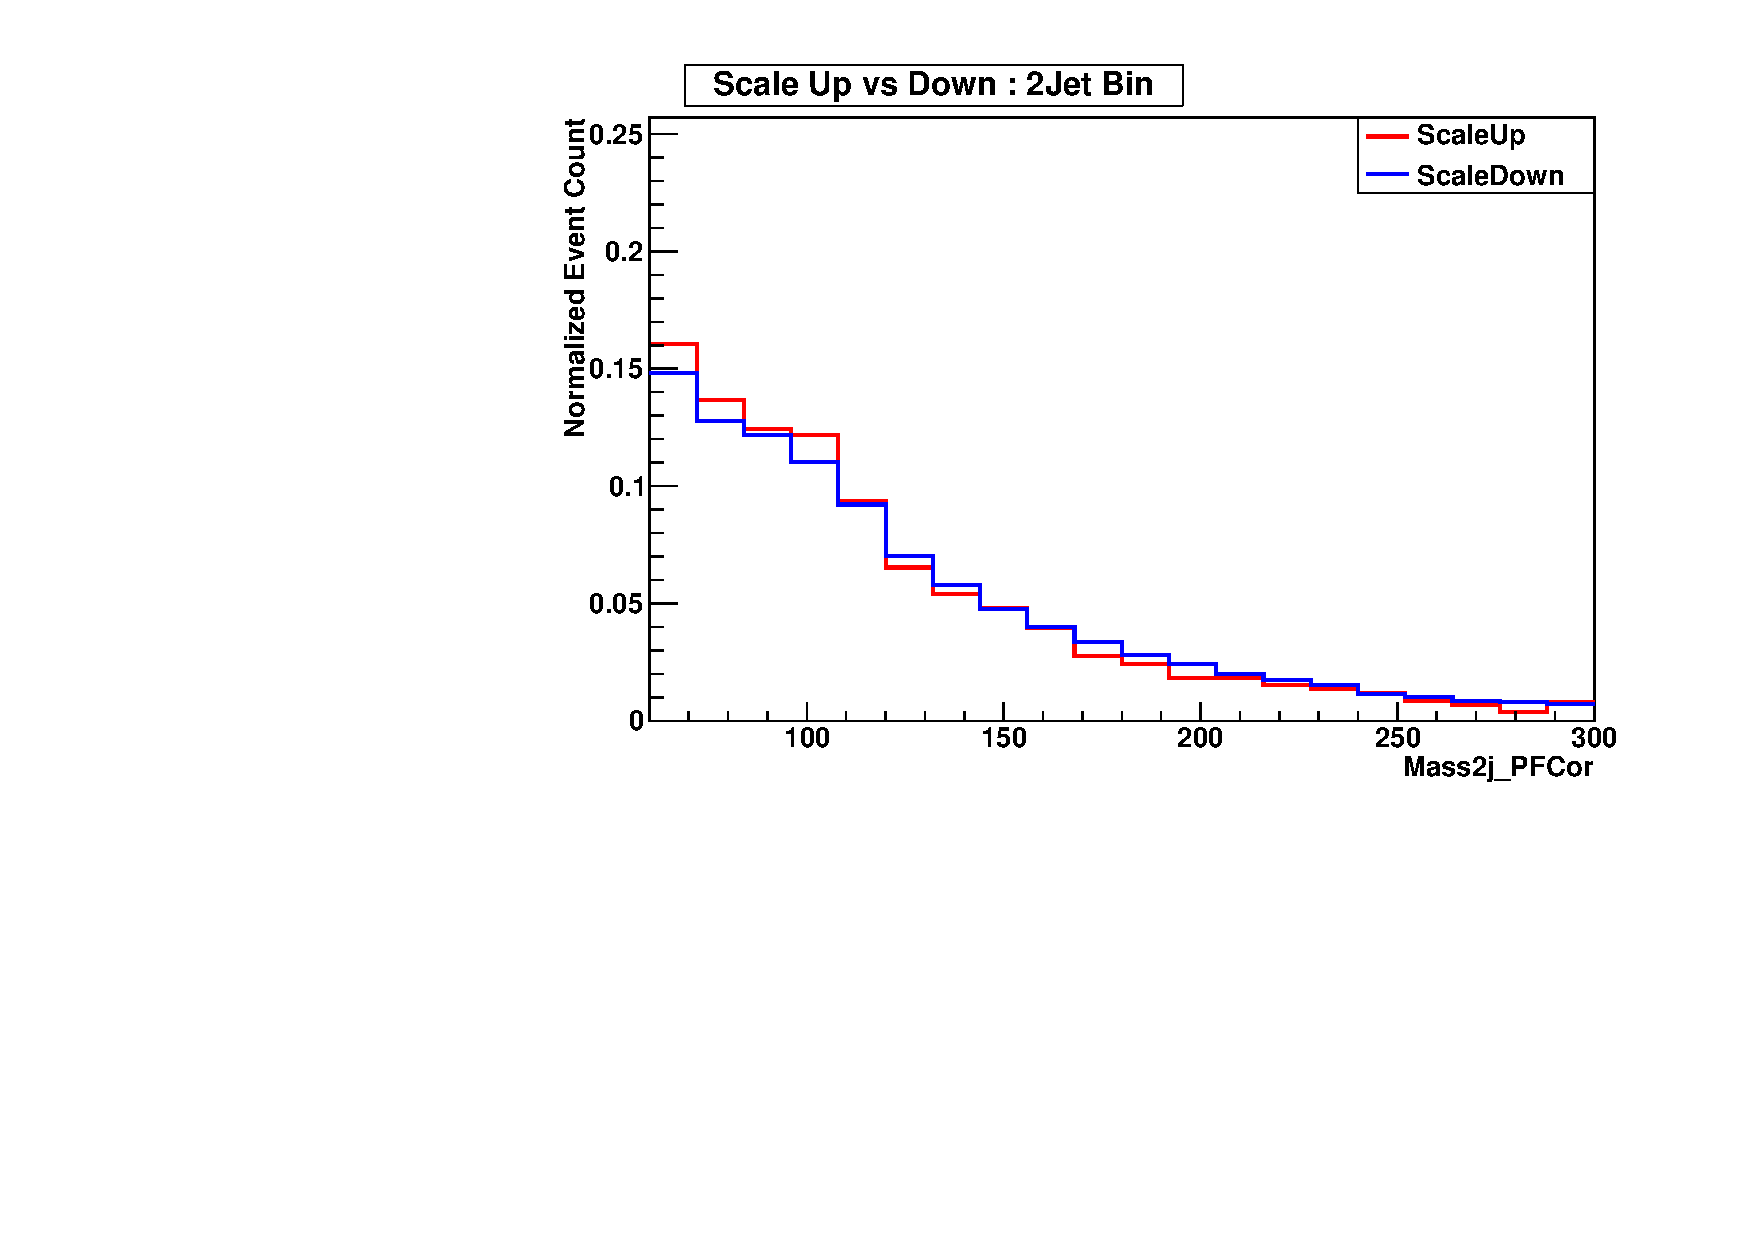
\includegraphics[width=0.48\textwidth]{figs/validation/ShapeComp_Scale2j.pdf}
\put(-0.80,0.0){(a)} 
\unitlength=0.33\linewidth
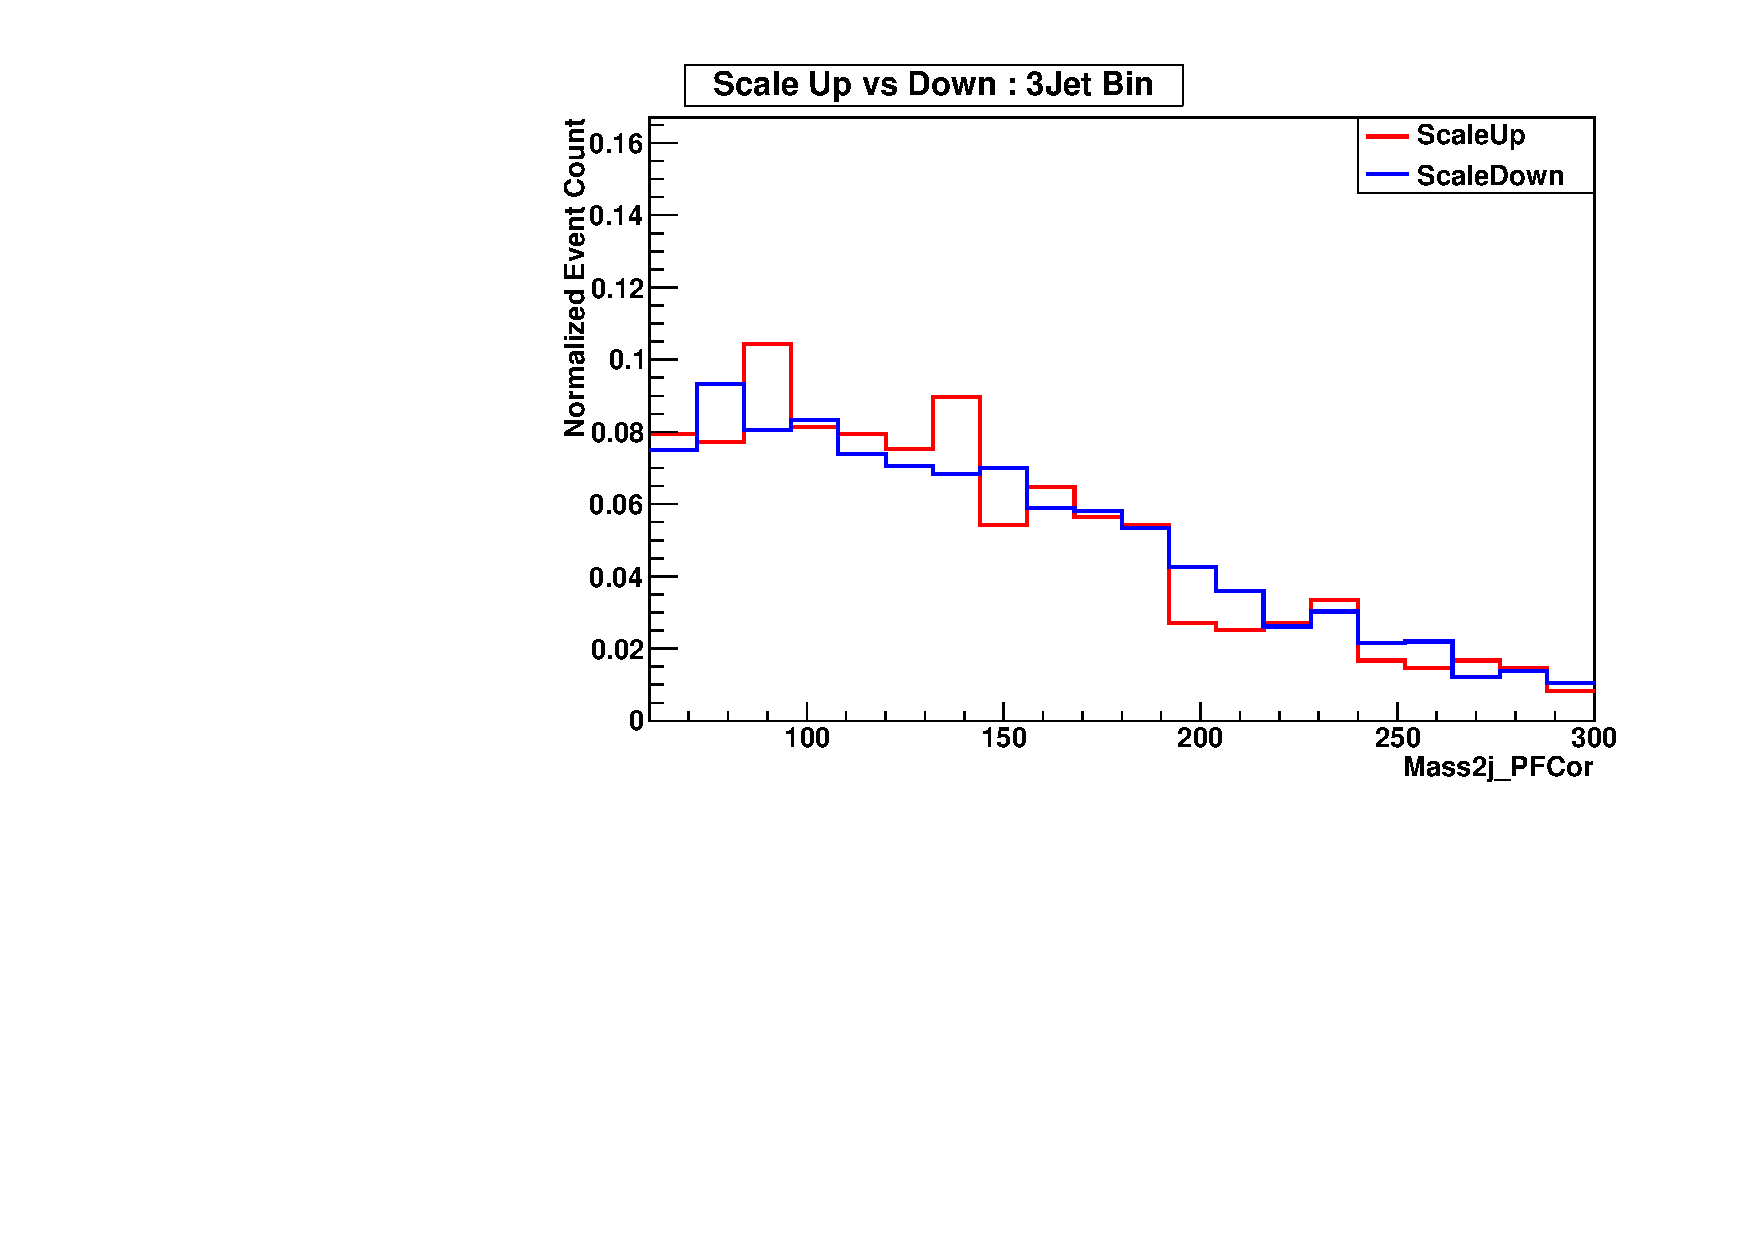
\includegraphics[width=0.48\textwidth]{figs/validation/ShapeComp_Scale3j.pdf}
\put(-0.80,0.0){(b)} \\
\unitlength=0.33\linewidth
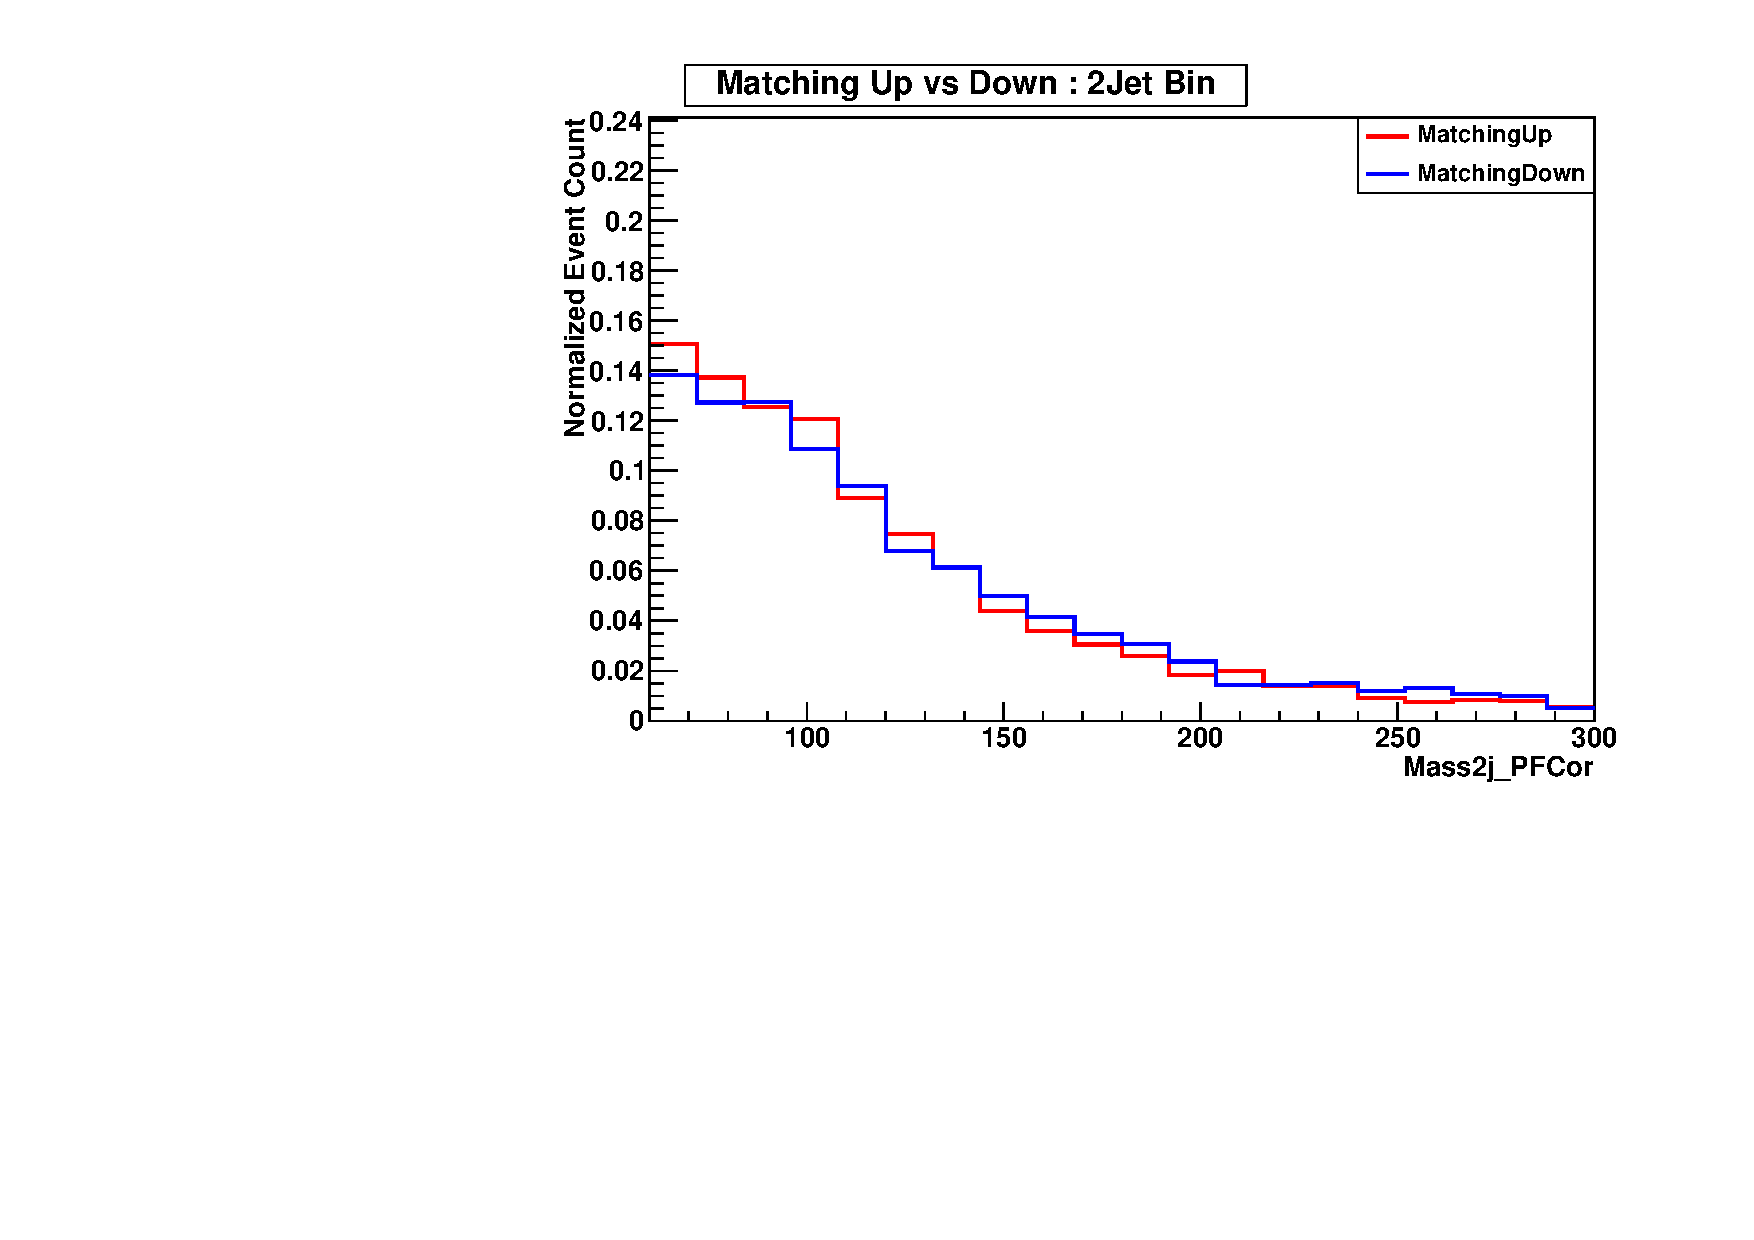
\includegraphics[width=0.48\textwidth]{figs/validation/ShapeComp_Matching2j.pdf}
\put(-0.80,0.0){(c)} 
\unitlength=0.33\linewidth
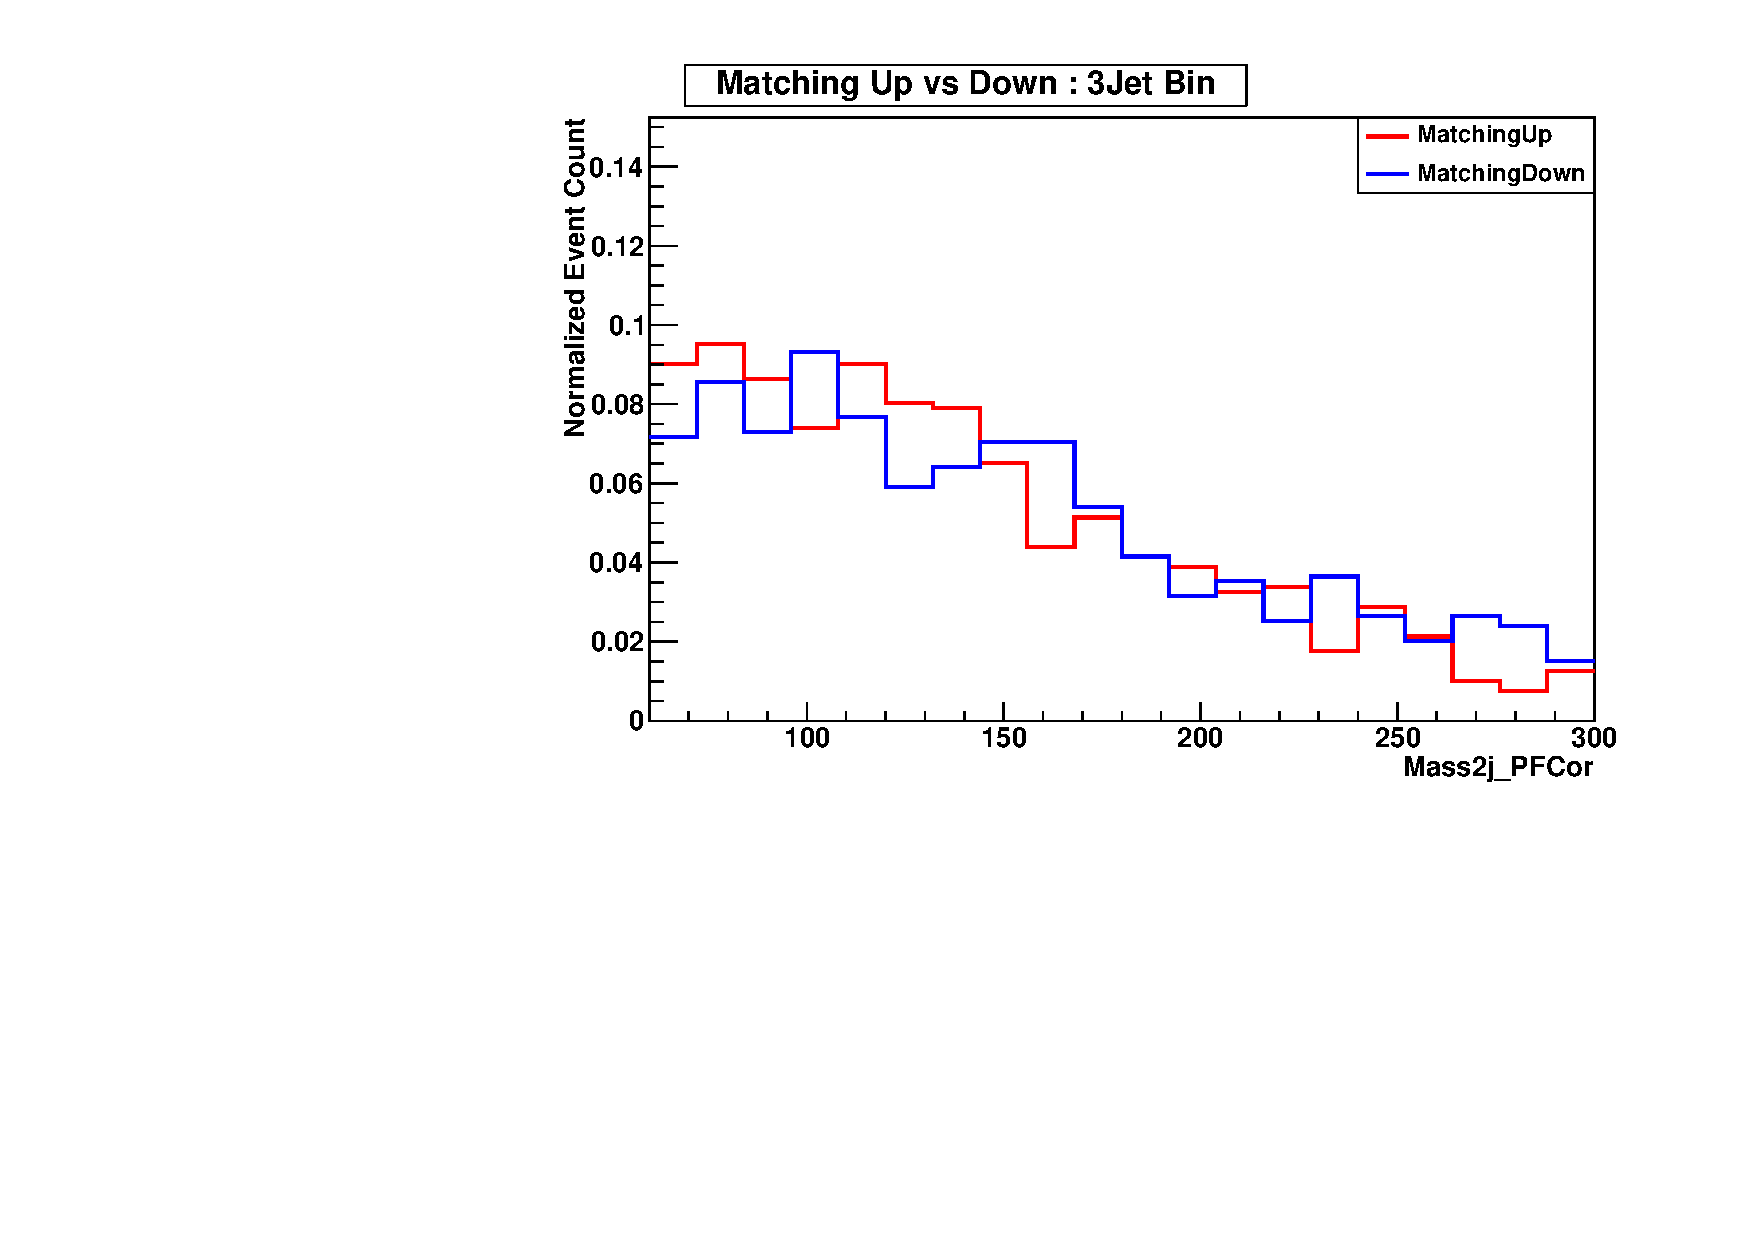
\includegraphics[width=0.48\textwidth]{figs/validation/ShapeComp_Matching3j.pdf}
\put(-0.80,0.0){(d)} 
\caption{Comparison between Up and Down shapes for: (a) scale - 2-jet bin, (b) scale - 3-jet bin, (c) matching - 2-jet bin, (d) matching - 3-jet bin.} 
\label{fig:Validation_fMUfSU_ShapeComparisonUpVsDown}}
\end{figure}
%%%%%%%
%%%%%%%%%%%%%%%%%%%%%%%%%%%%
%%%%%%%
\begin{figure}[h!] {\centering
\unitlength=0.33\linewidth
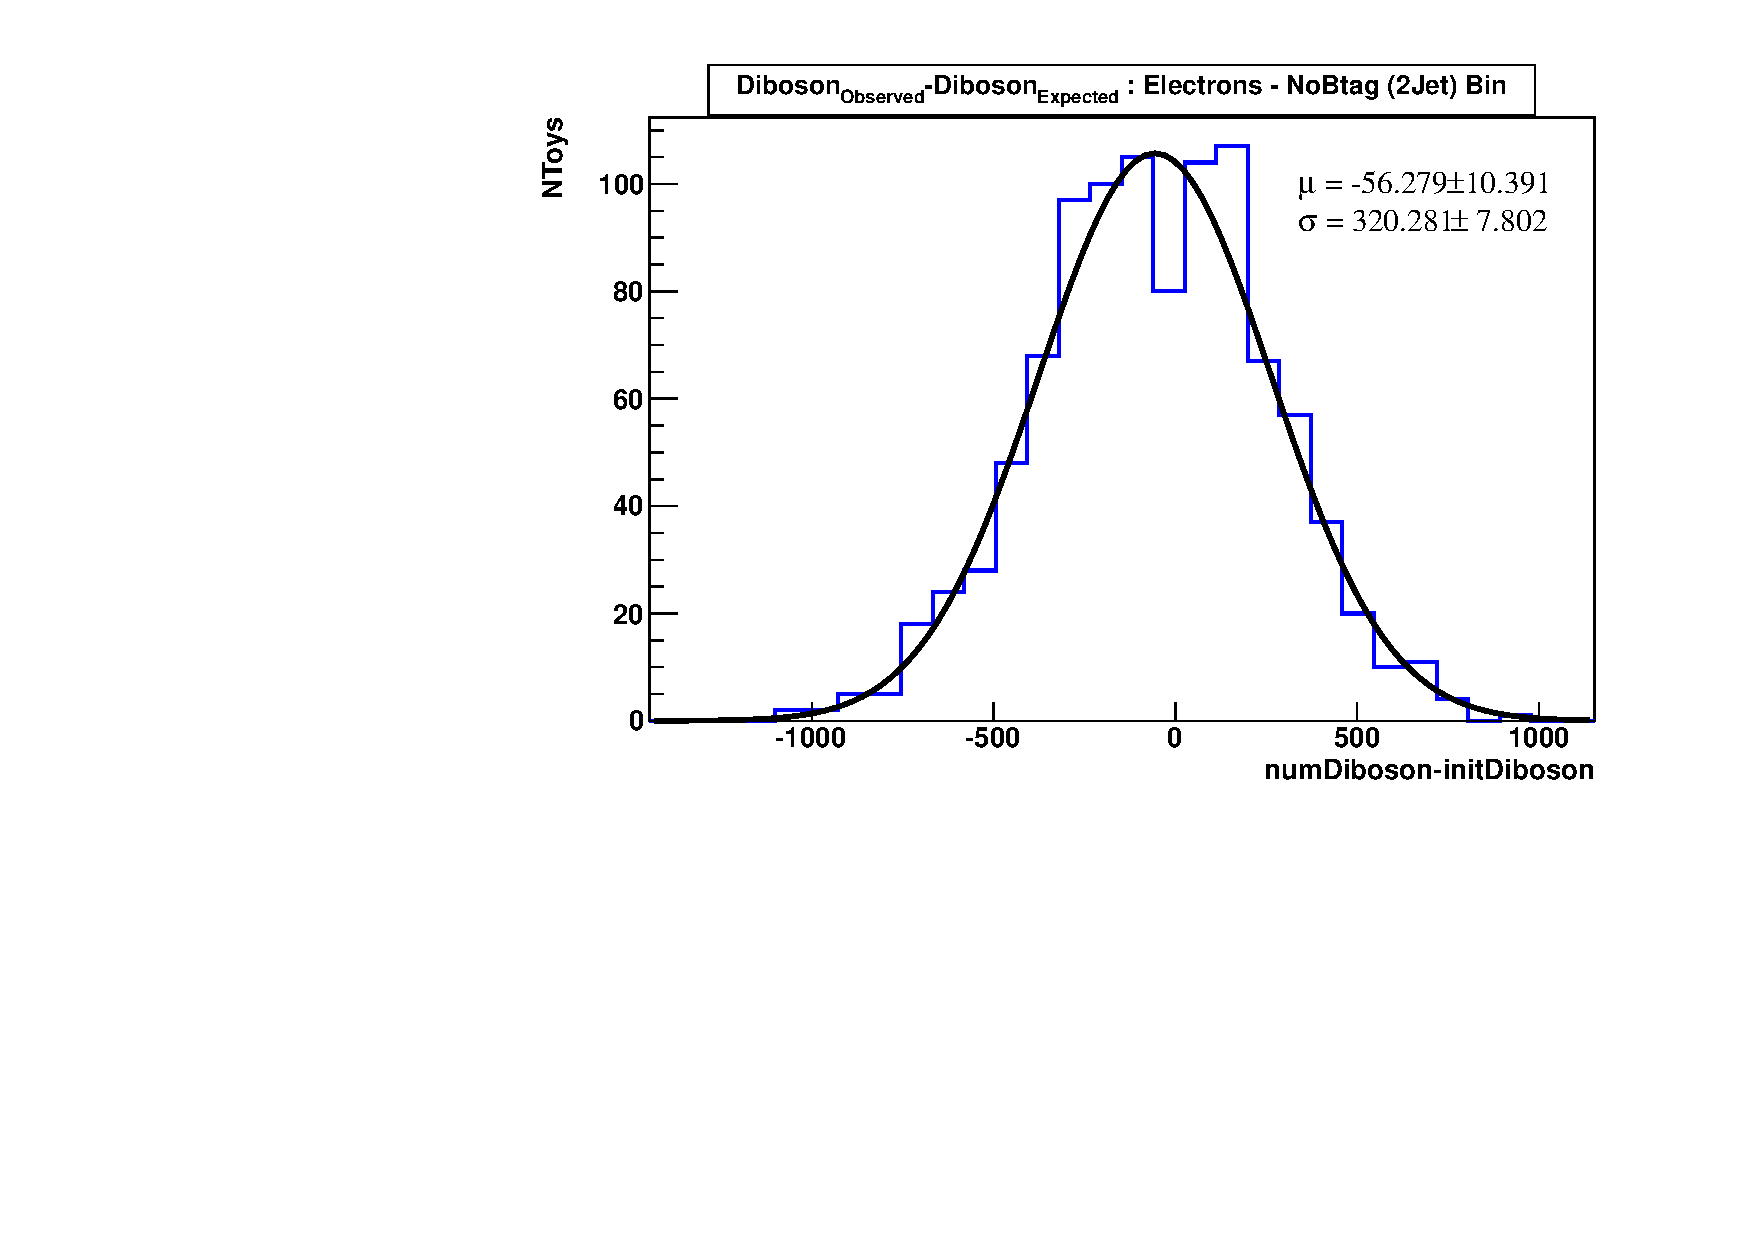
\includegraphics[width=0.96\textwidth]{figs/validation/DibosonYield_Validation_el_NoBtag_2j.pdf}
\put(-1.5,0.0){(a)} \\
\unitlength=0.33\linewidth
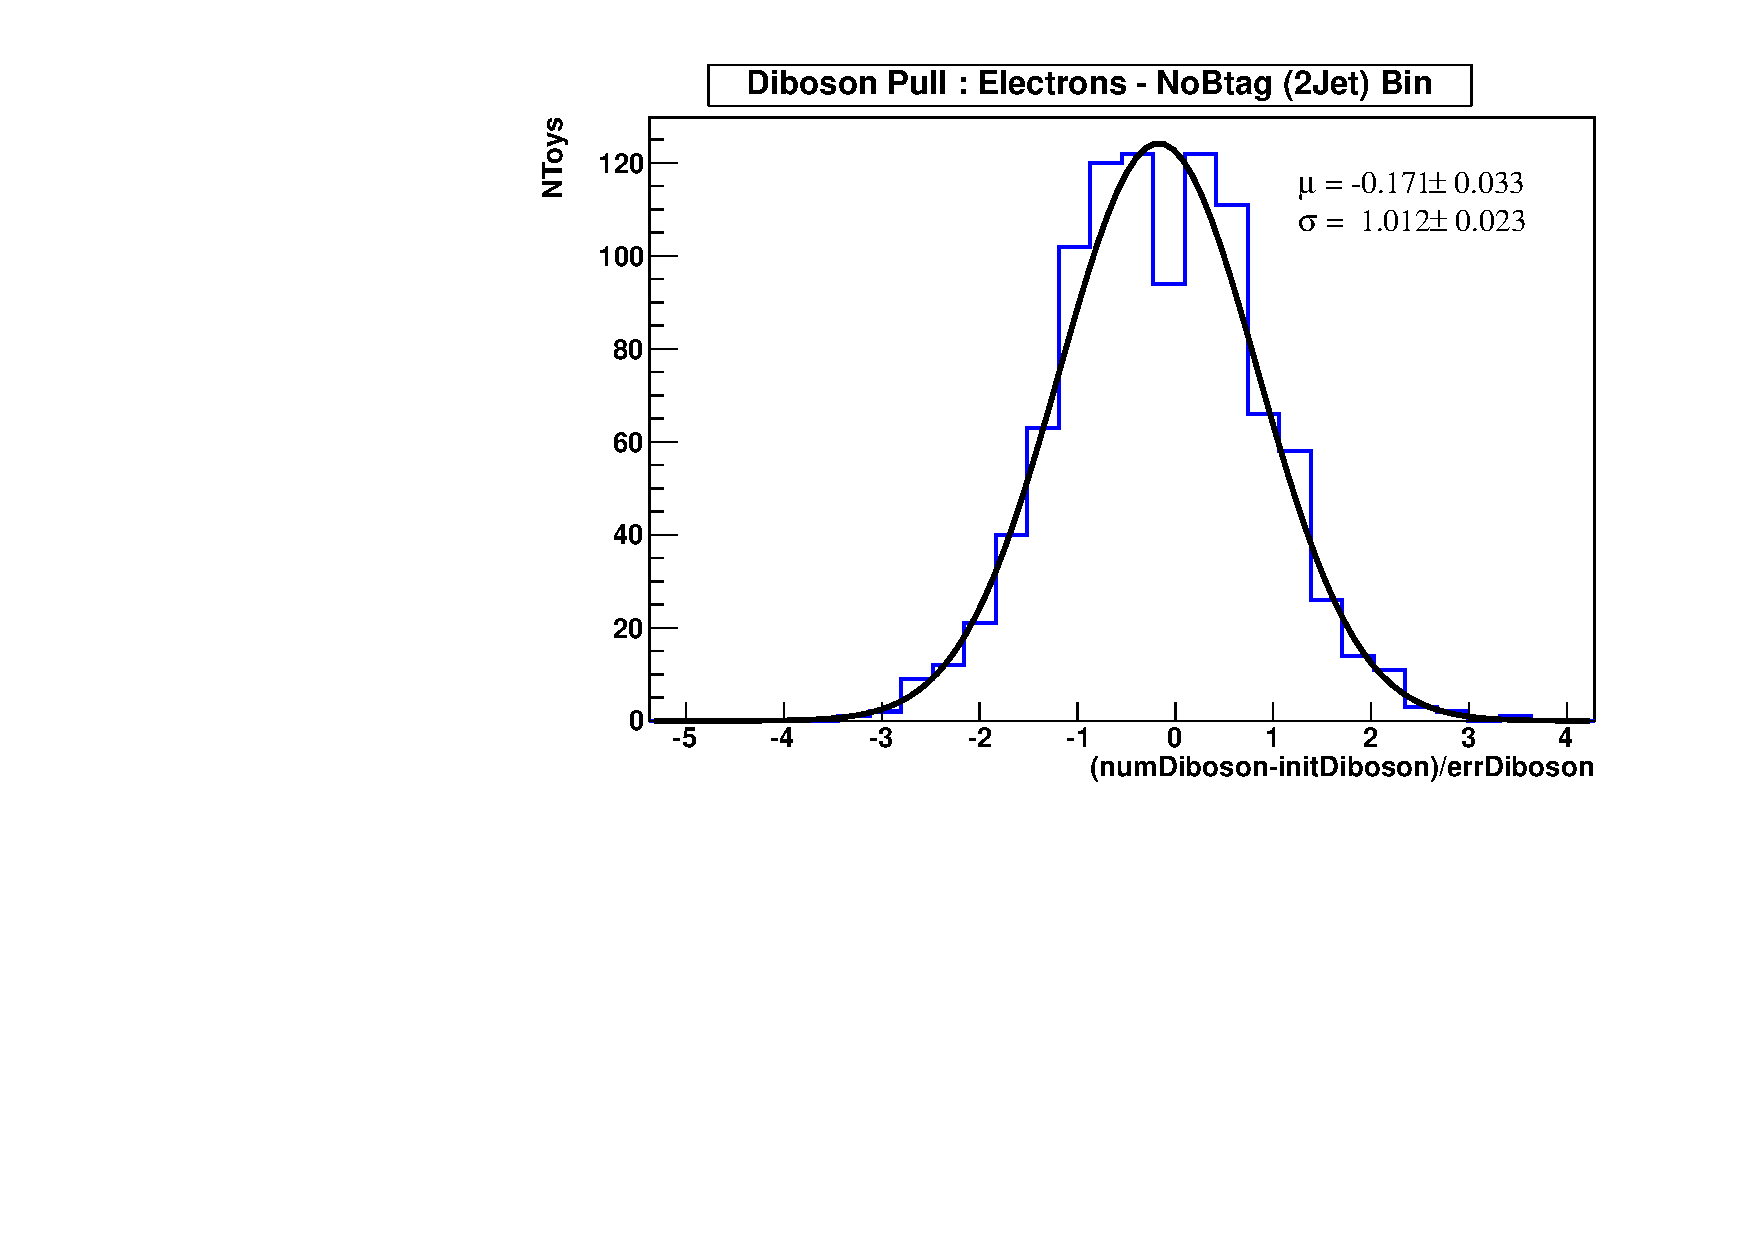
\includegraphics[width=0.96\textwidth]{figs/validation/DibosonPull_Validation_el_NoBtag_2j.pdf}
\put(-1.5,0.0){(b)} \\
\caption{Fit validation in the untagged (2-jet) bin of the electron channel, using 1000 Toy MC datasets. Diboson (a) Fitted-Given Yield, (b) Pull=(Fitted-Given)/Error.} 
\label{fig:DibosonValidation_el_NoBTag}}
\end{figure}
%%%%%%%
%%%%%%%
\begin{figure}[h!] {\centering
\unitlength=0.33\linewidth
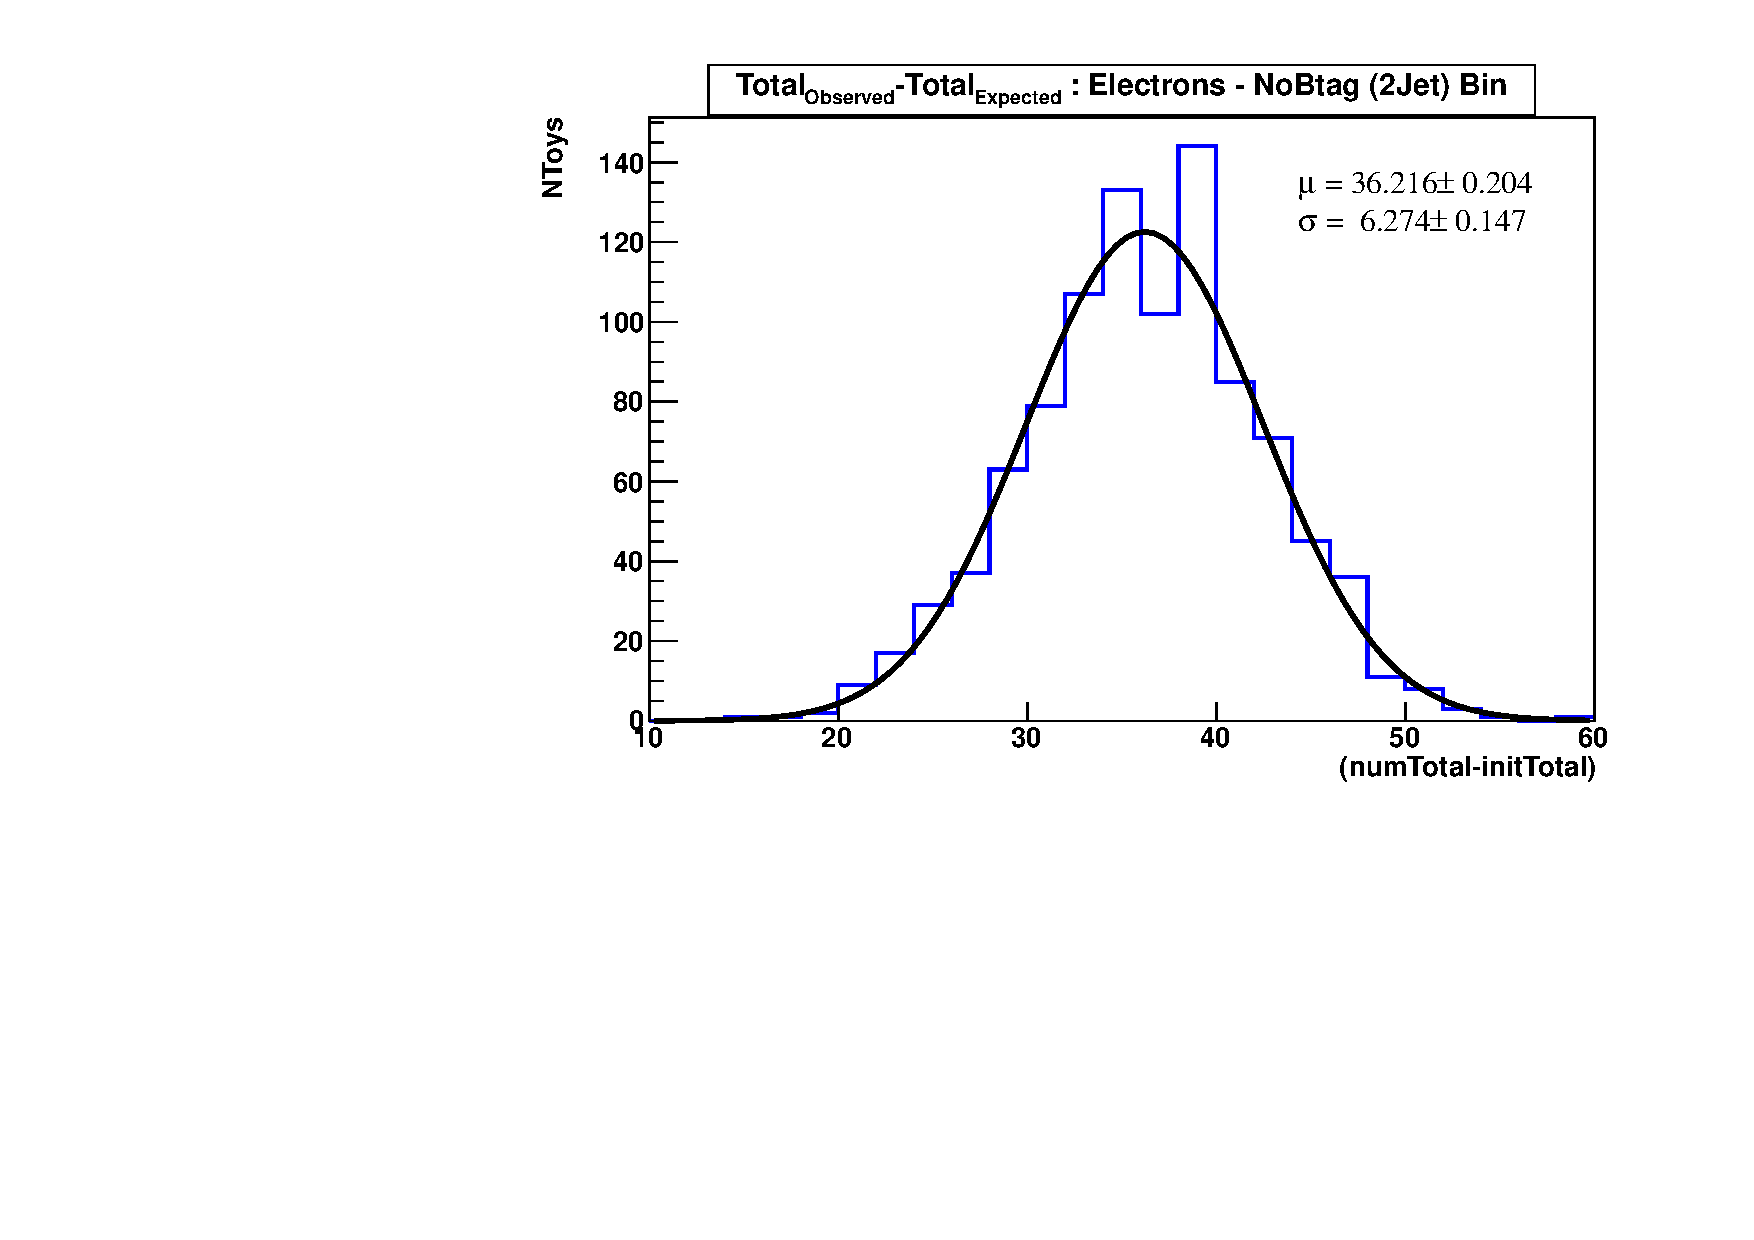
\includegraphics[width=0.48\textwidth]{figs/validation/TotalYield_Validation_el_NoBtag_2j.pdf}
\put(-0.80,0.0){(a)}
\unitlength=0.33\linewidth
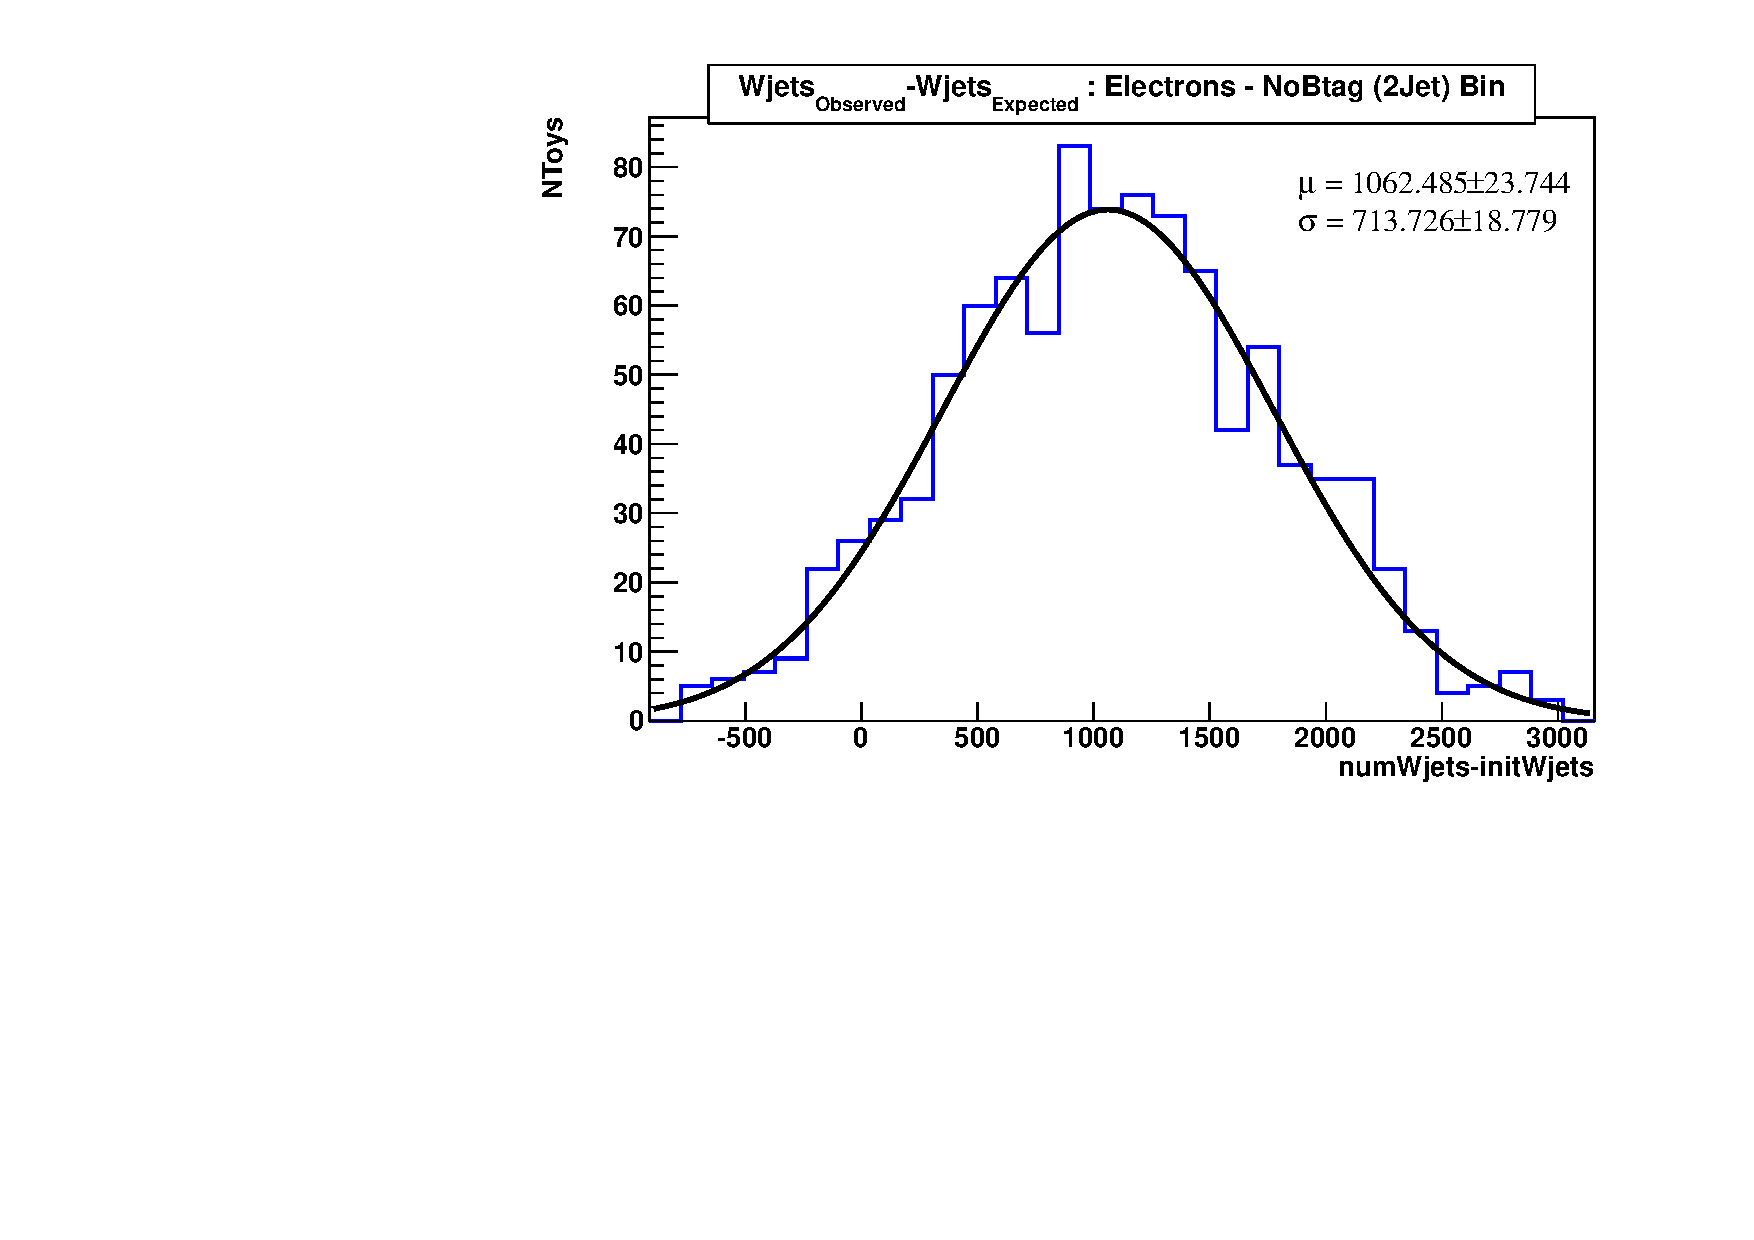
\includegraphics[width=0.48\textwidth]{figs/validation/WjetsYield_Validation_el_NoBtag_2j.pdf}
\put(-0.80,0.0){(b)}\\ 
\unitlength=0.33\linewidth
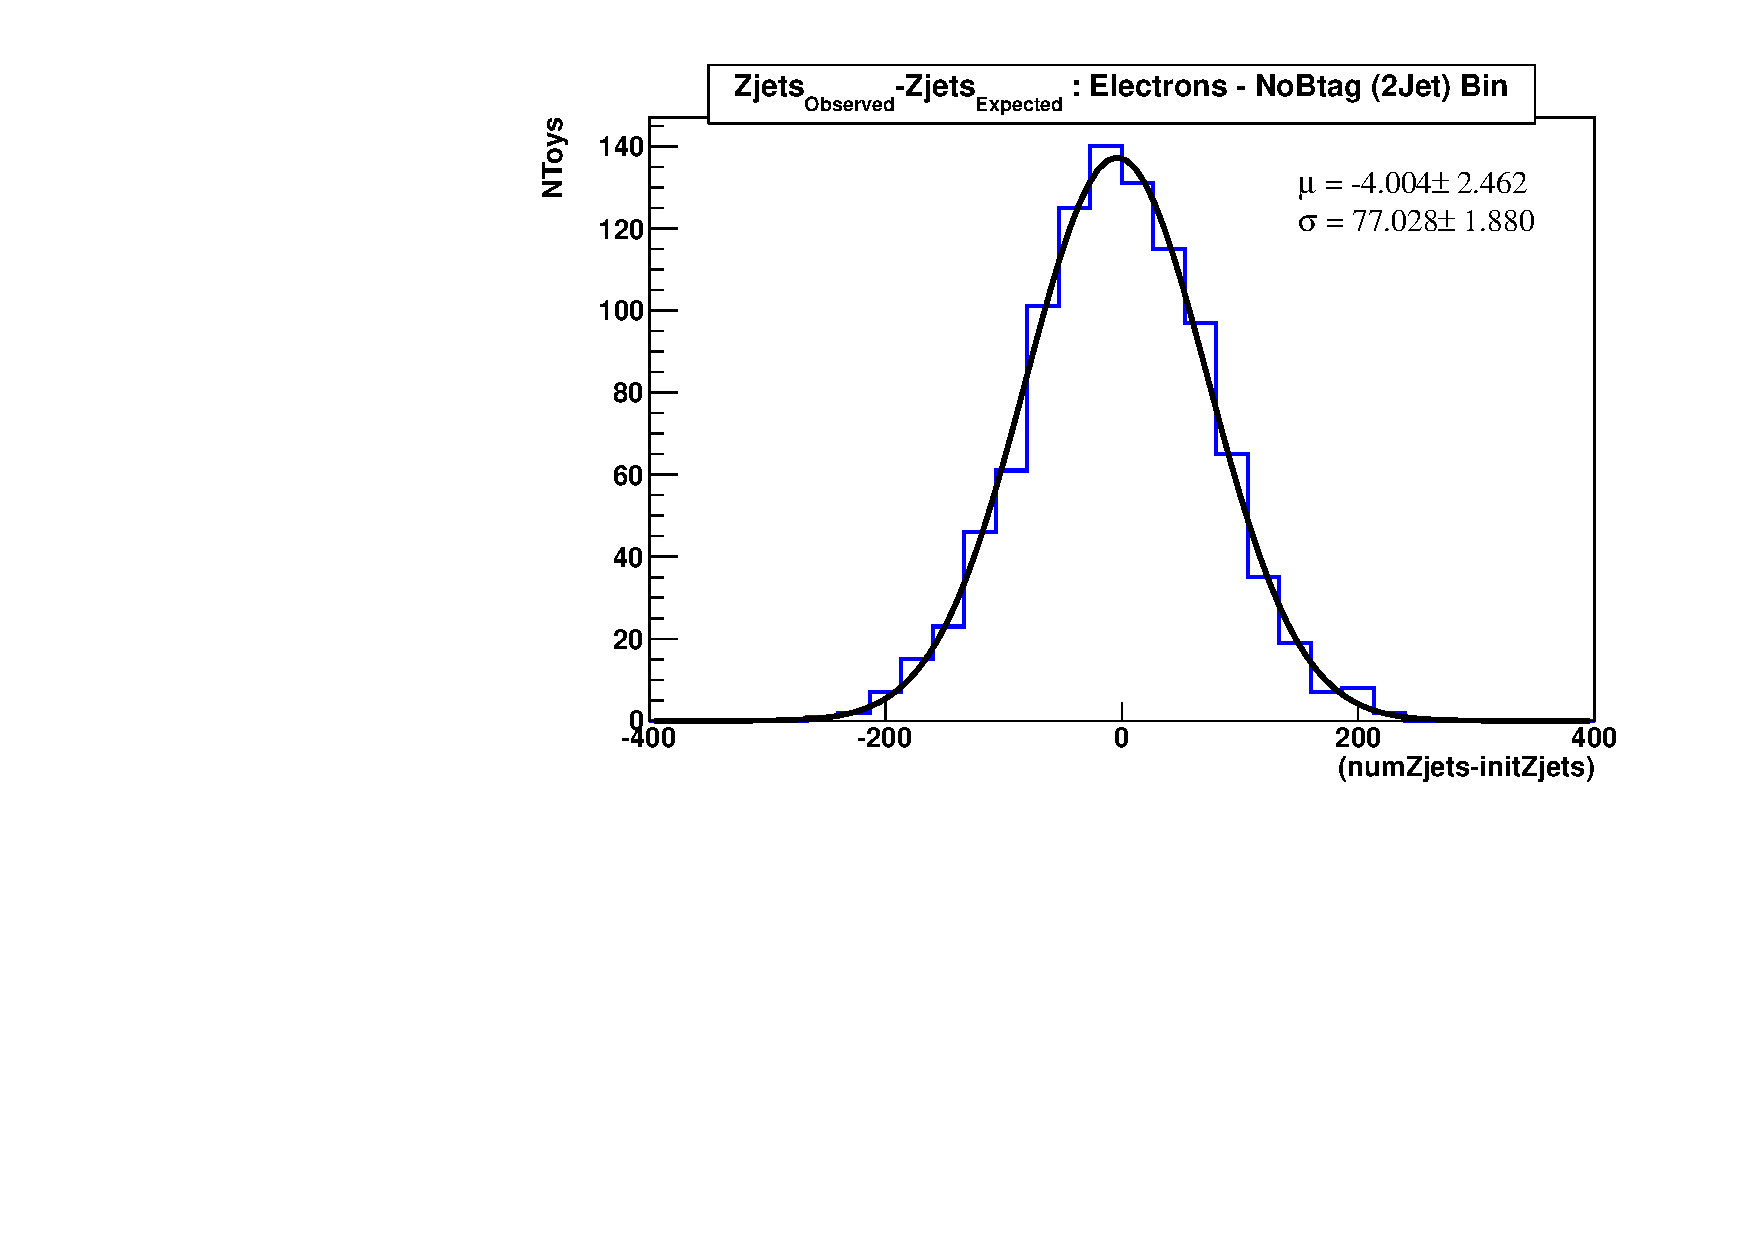
\includegraphics[width=0.48\textwidth]{figs/validation/ZjetsYield_Validation_el_NoBtag_2j.pdf}
\put(-0.80,0.0){(c)}
\unitlength=0.33\linewidth
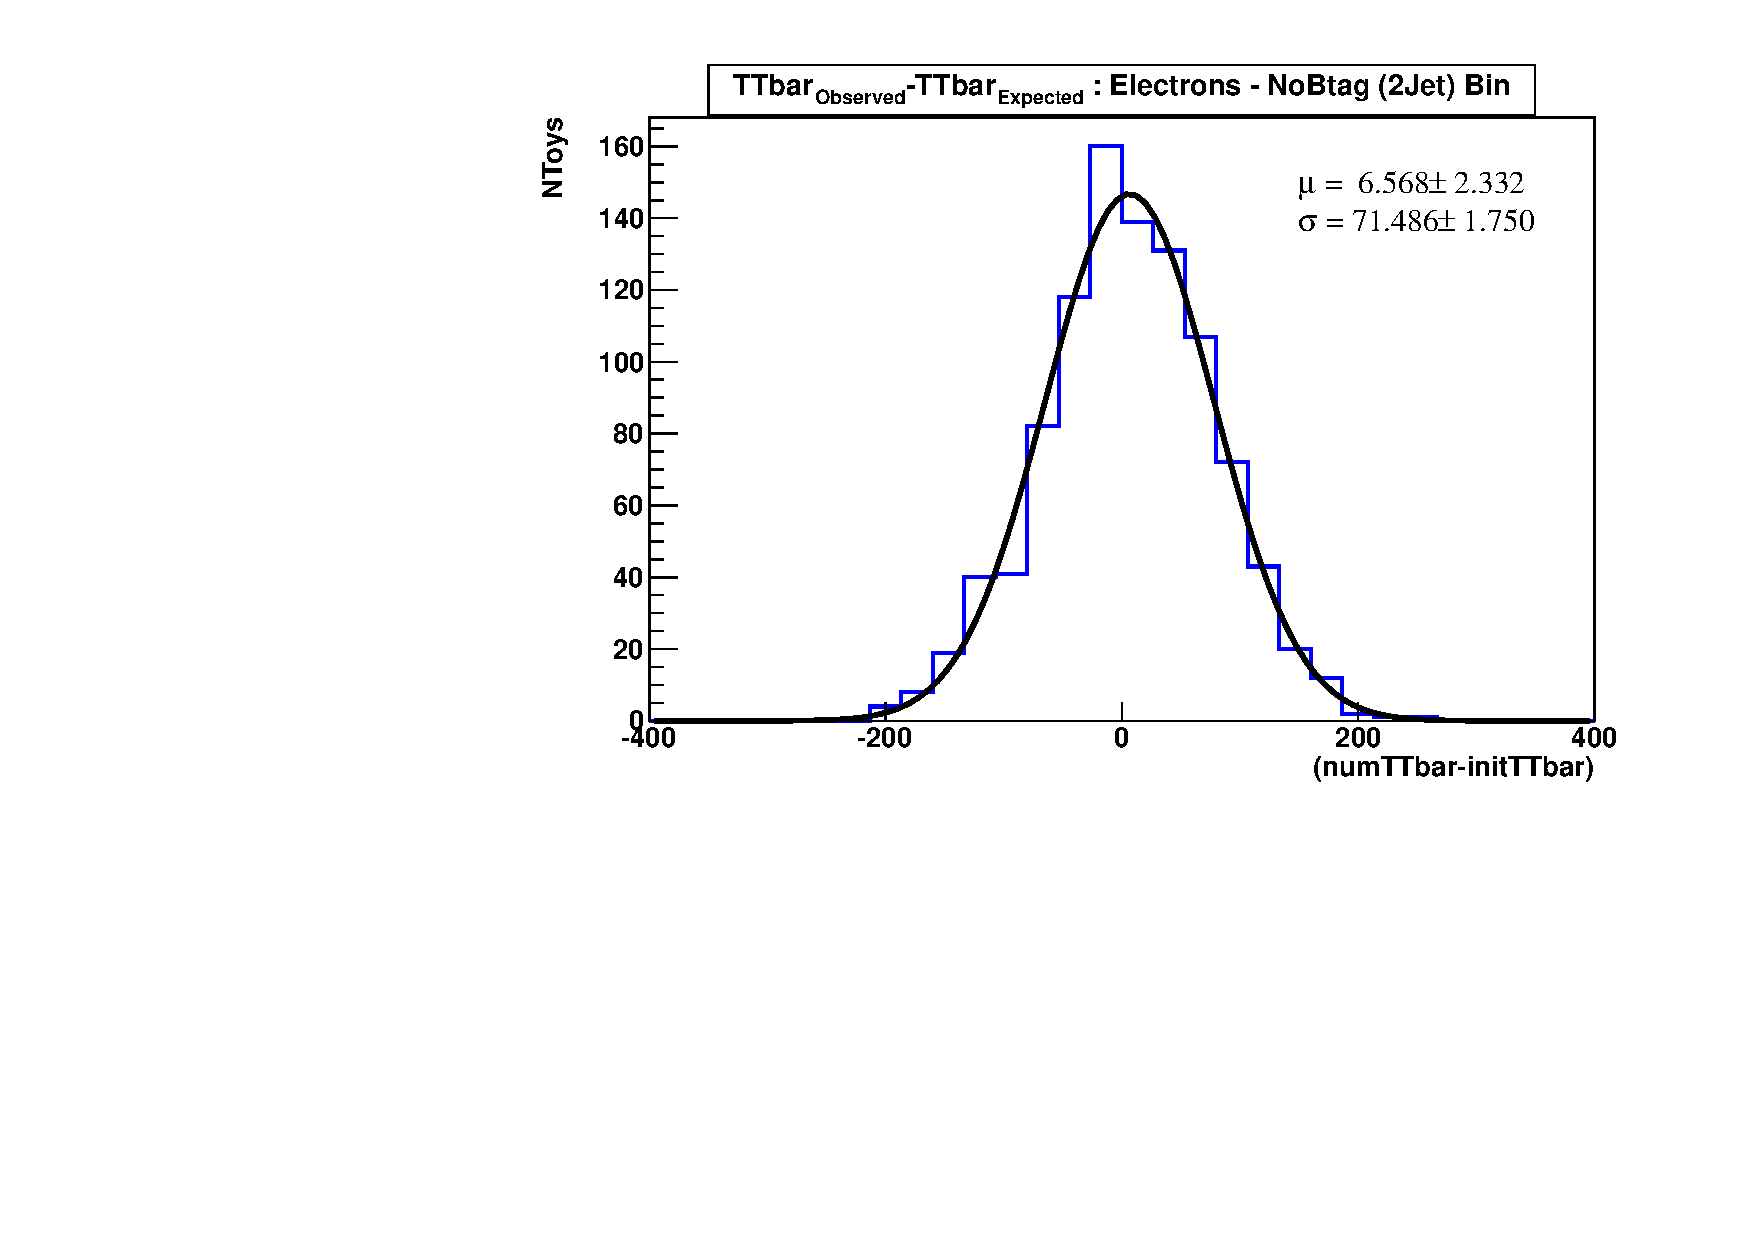
\includegraphics[width=0.48\textwidth]{figs/validation/TTbarYield_Validation_el_NoBtag_2j.pdf}
\put(-0.80,0.0){(d)}\\ 
\unitlength=0.33\linewidth
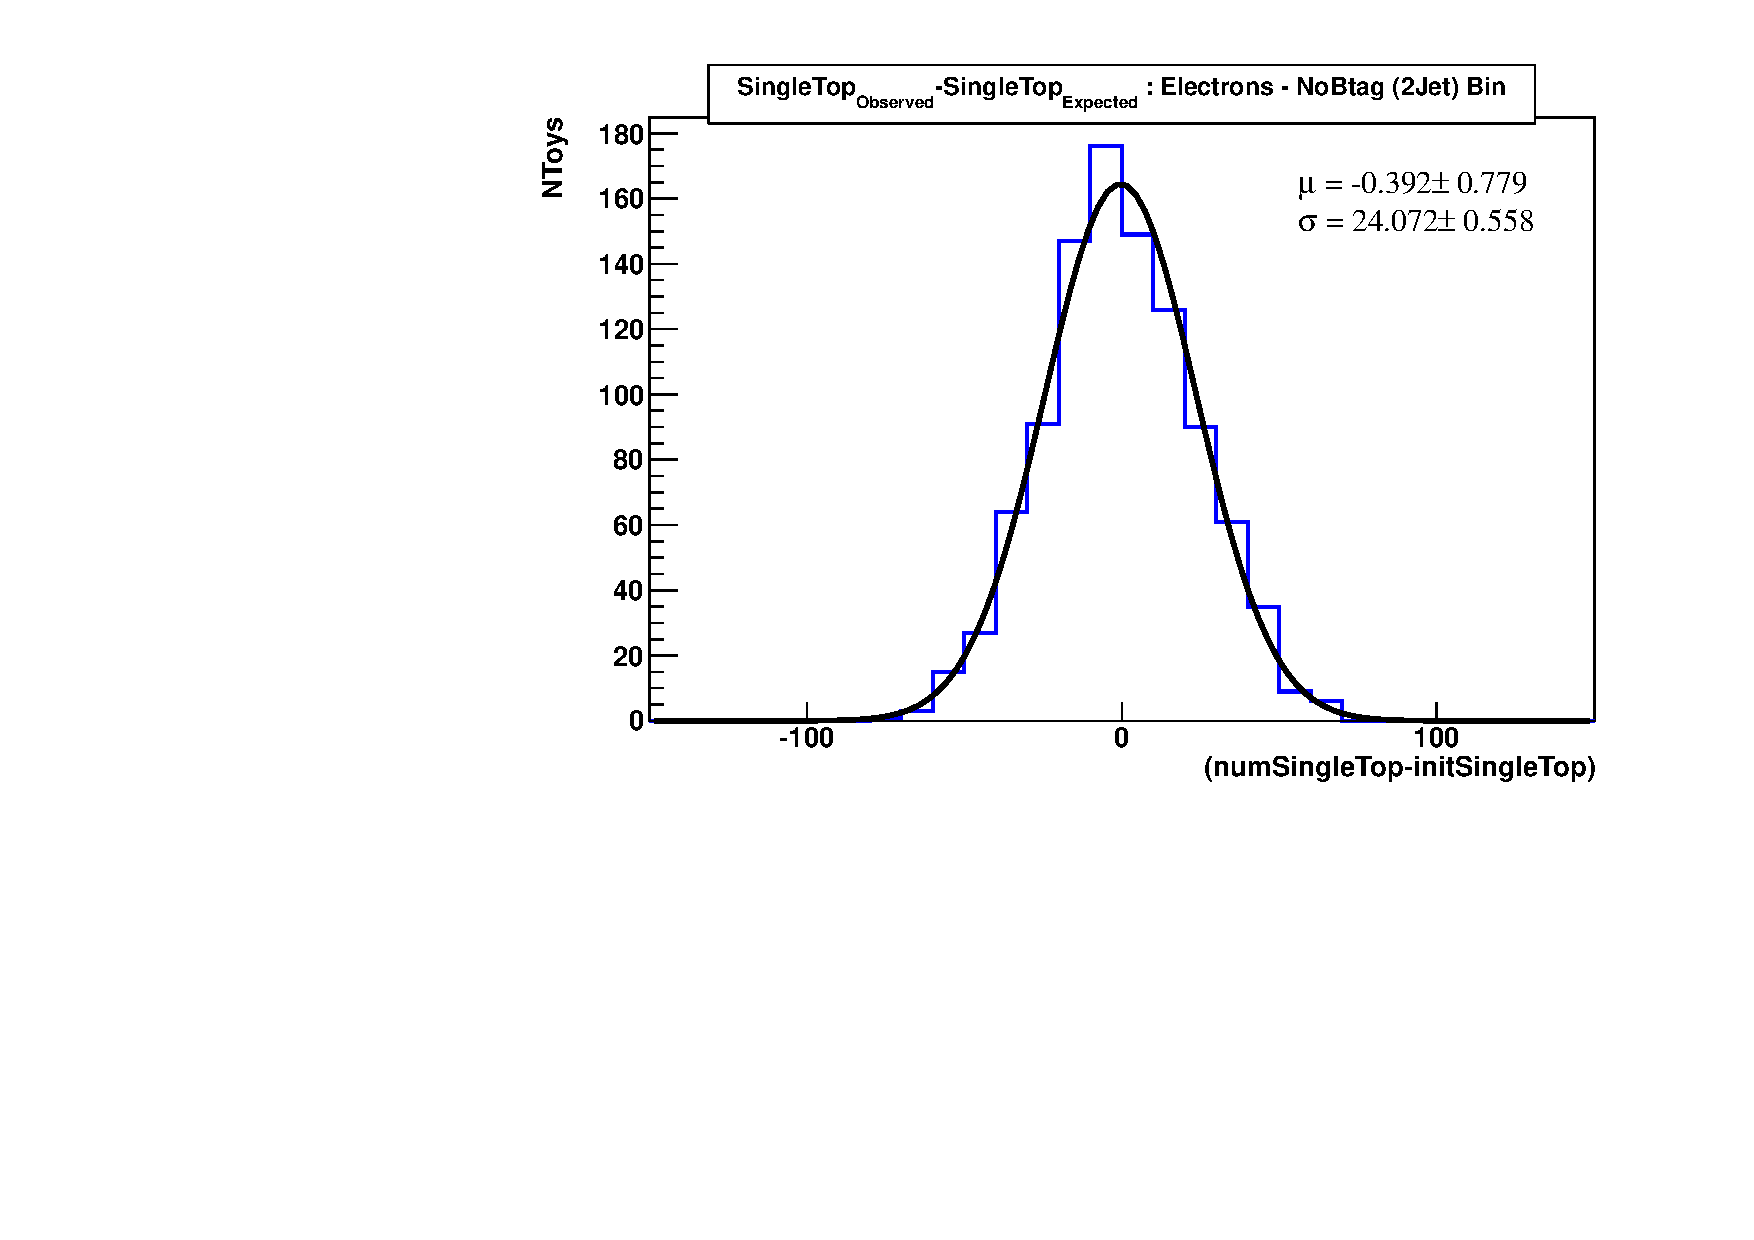
\includegraphics[width=0.48\textwidth]{figs/validation/SingleTopYield_Validation_el_NoBtag_2j.pdf}
\put(-0.80,0.0){(e)} 
\unitlength=0.33\linewidth
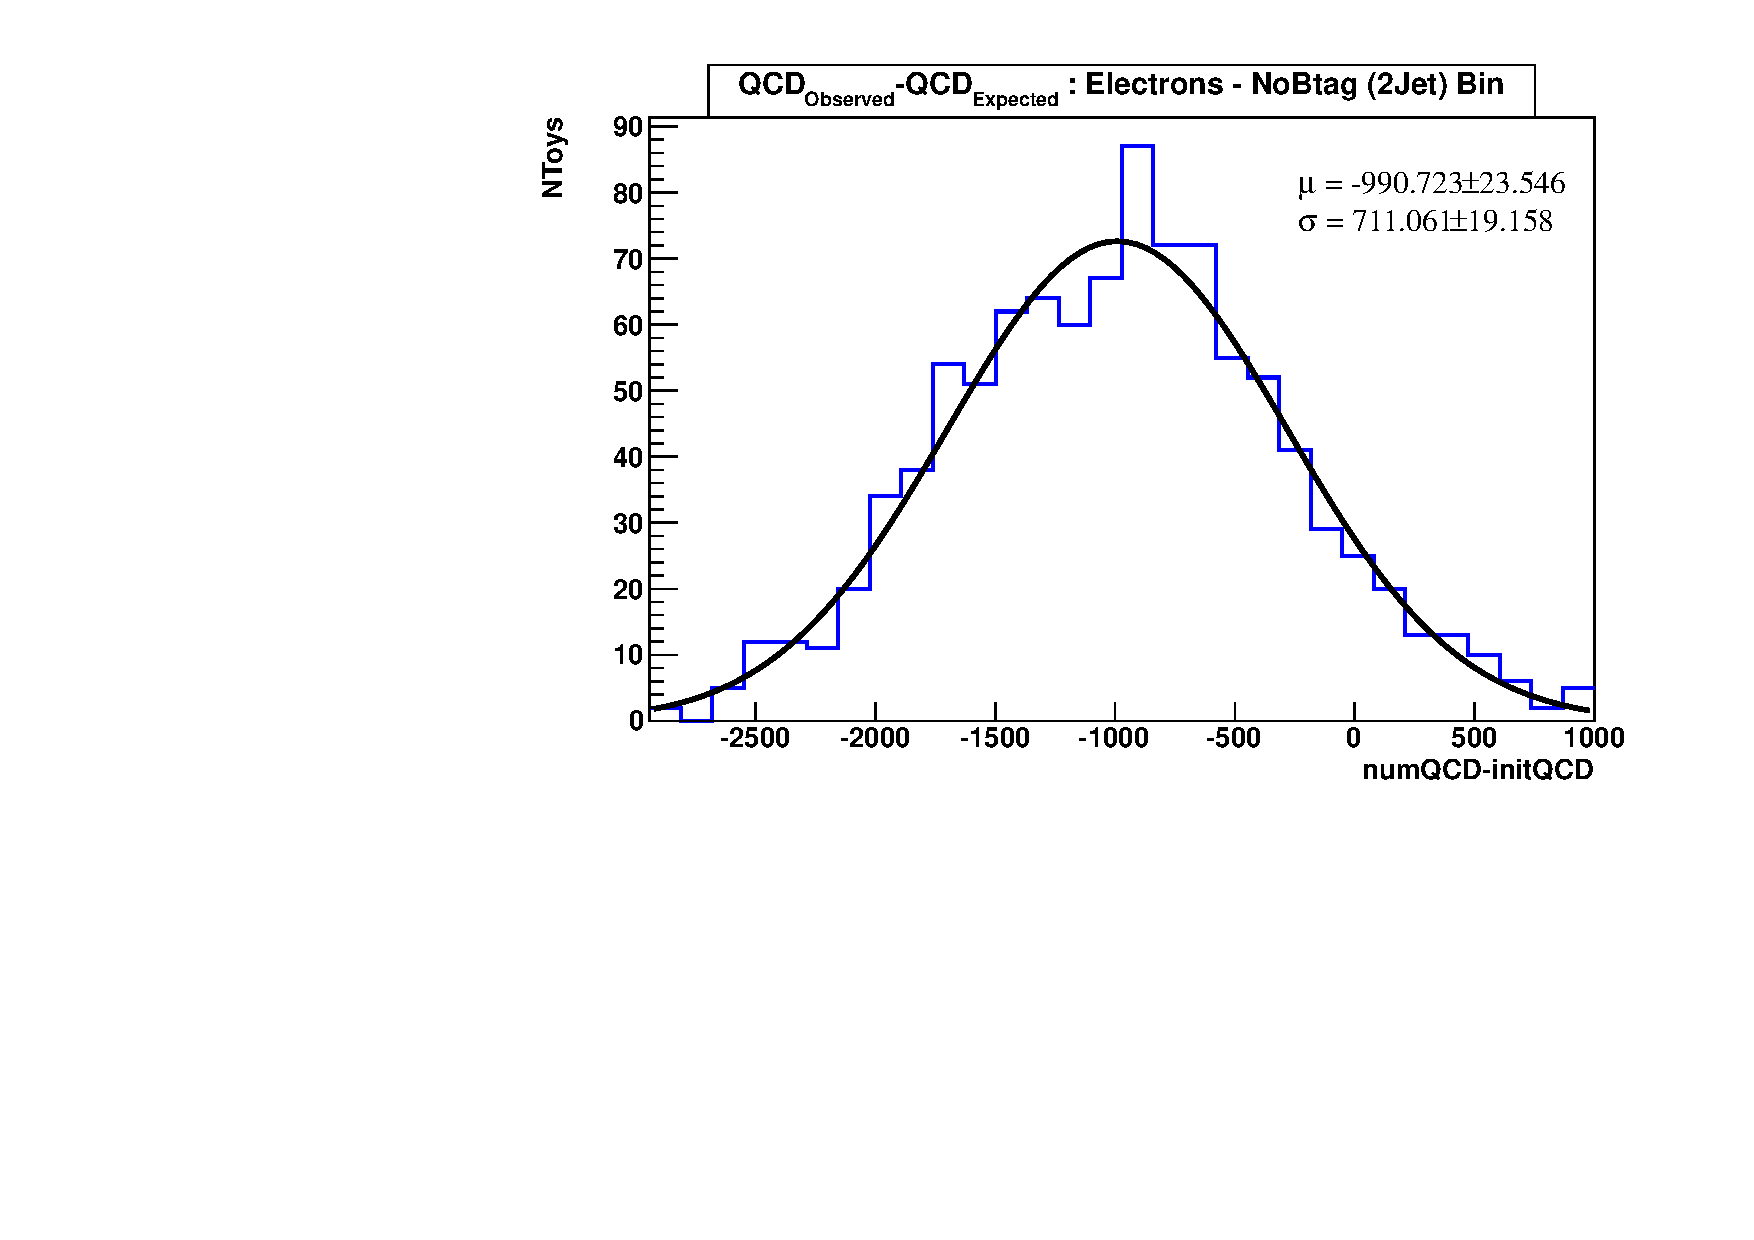
\includegraphics[width=0.48\textwidth]{figs/validation/QCDYield_Validation_el_NoBtag_2j.pdf}
\put(-0.80,0.0){(f)}\\
\unitlength=0.33\linewidth
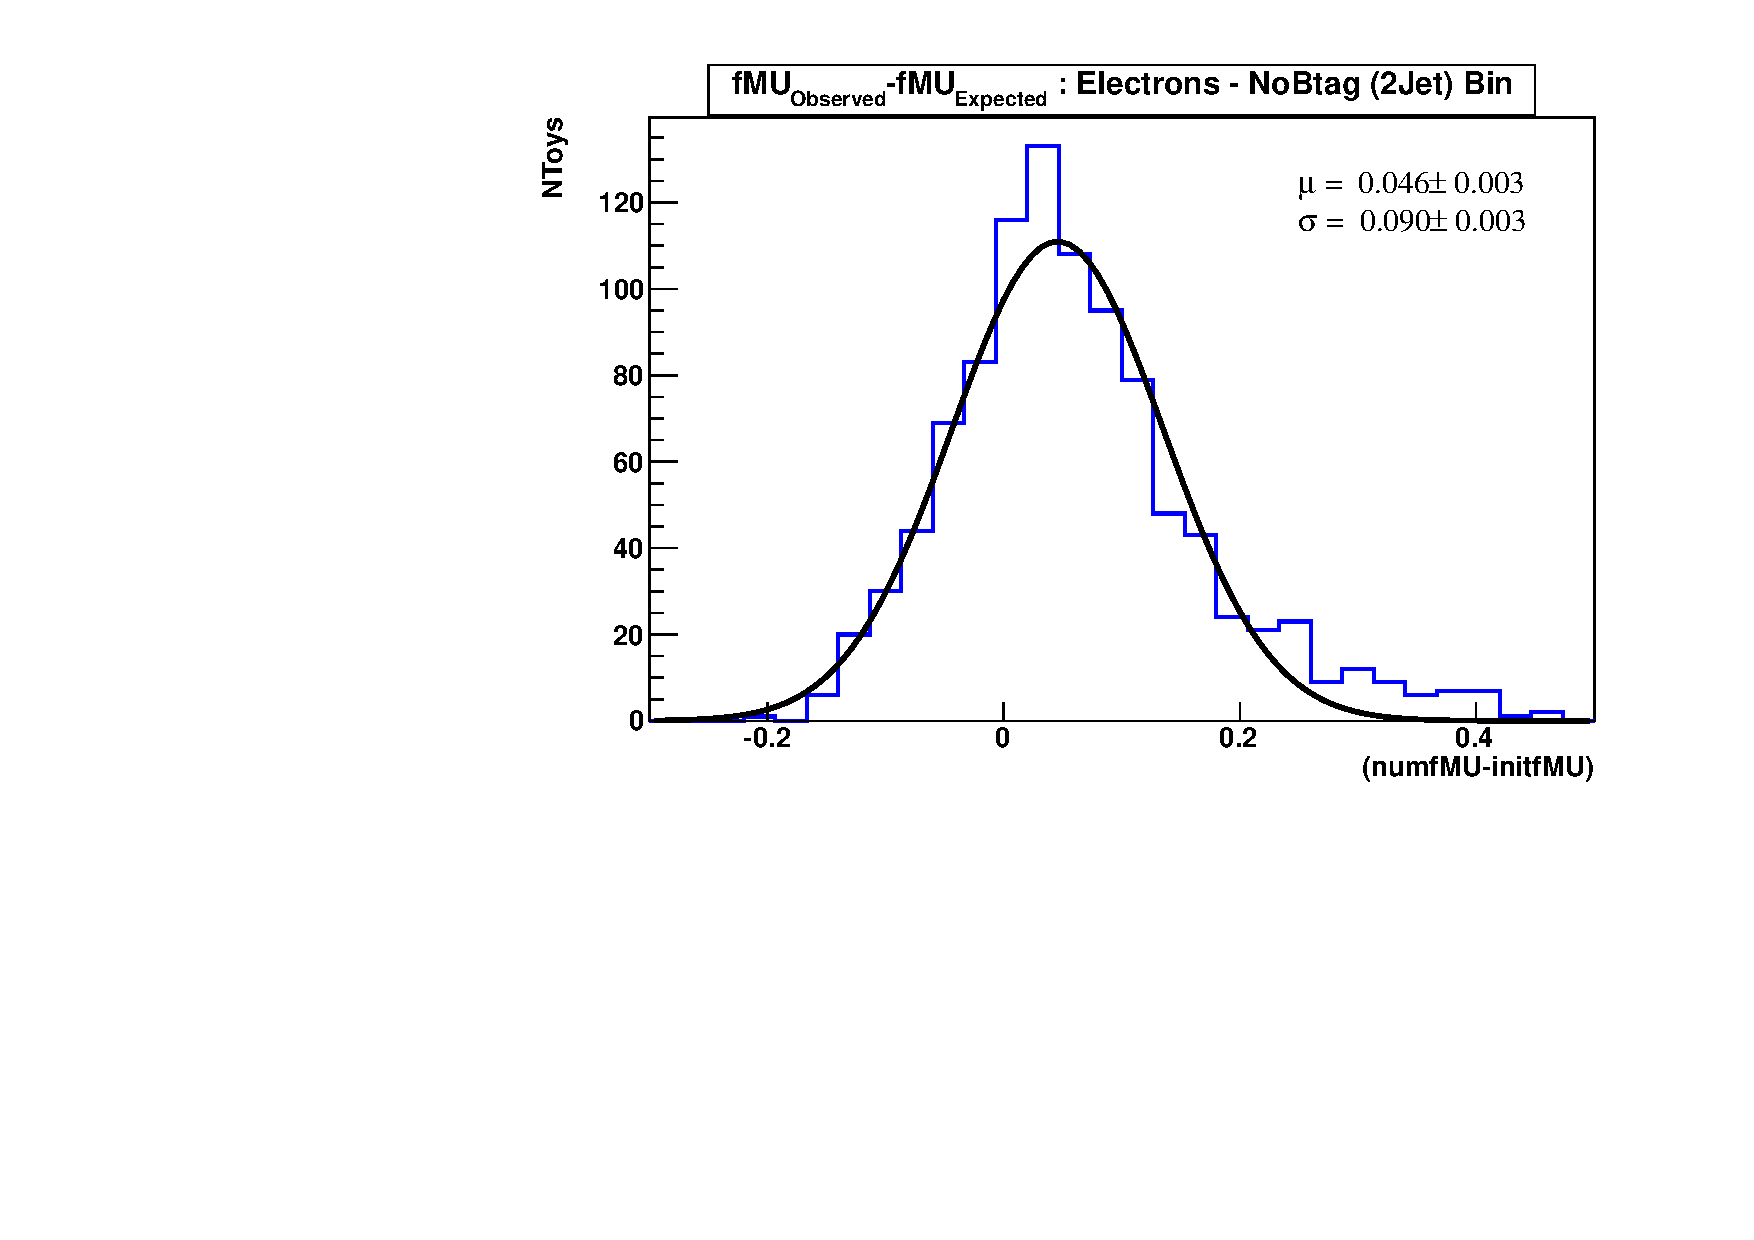
\includegraphics[width=0.48\textwidth]{figs/validation/fMUYield_Validation_el_NoBtag_2j.pdf}
\put(-0.80,0.0){(g)} 
\unitlength=0.33\linewidth
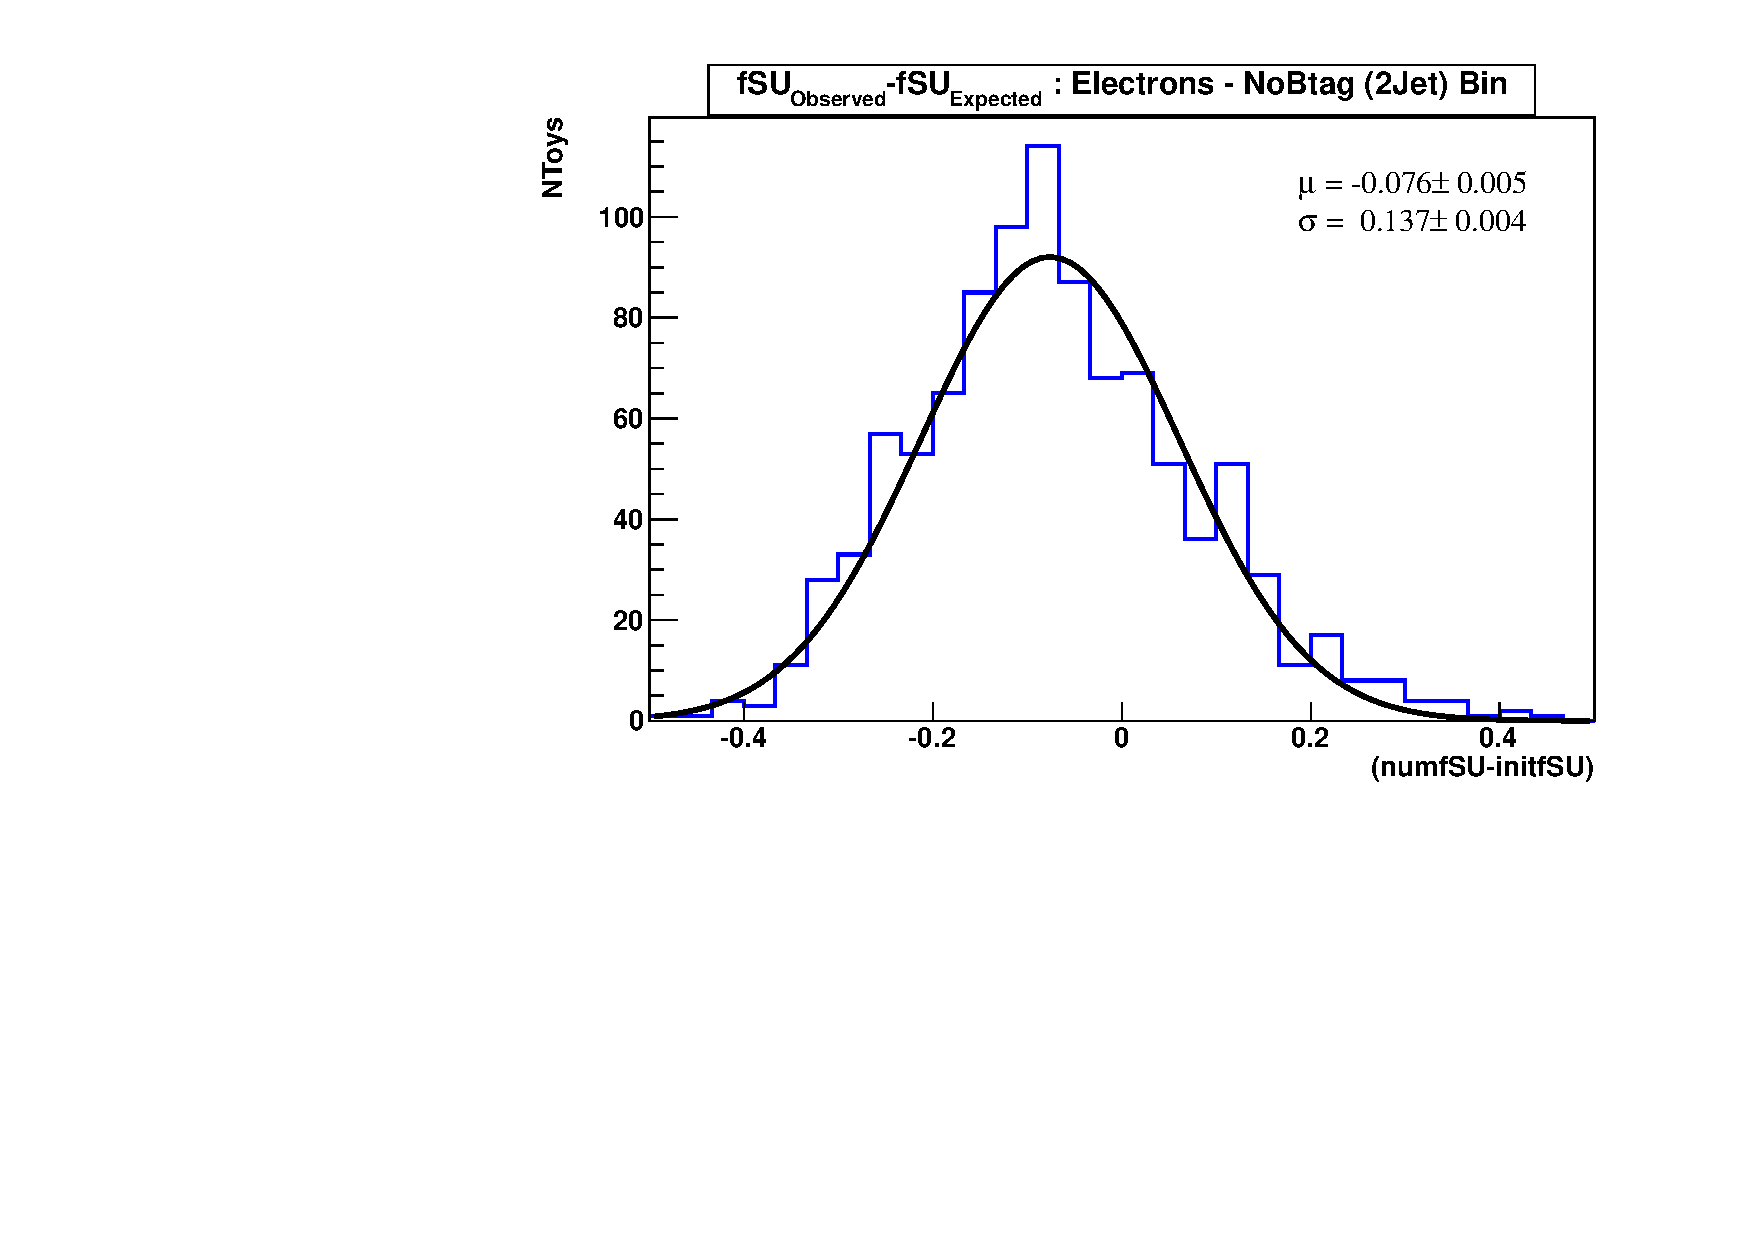
\includegraphics[width=0.48\textwidth]{figs/validation/fSUYield_Validation_el_NoBtag_2j.pdf}
\put(-0.80,0.0){(h)} 
\caption{Fit validation in the  untagged (2-jet) bin of the electron channel, using 1000 Toy MC datasets. Fitted-Given yields for: (a) Total, (b) W+jets, (c) Z+jets, (d) $t\bar{t}$, (e) SingleTop, (f) QCD, (g) Matching Up Fraction, (h) Scale Up Fraction.} 
\label{fig:Validation_Yields_el_NoBTag_2j}}
\end{figure}
%%%%%%%
%%%%%%%
\begin{figure}[h!] {\centering
\unitlength=0.33\linewidth
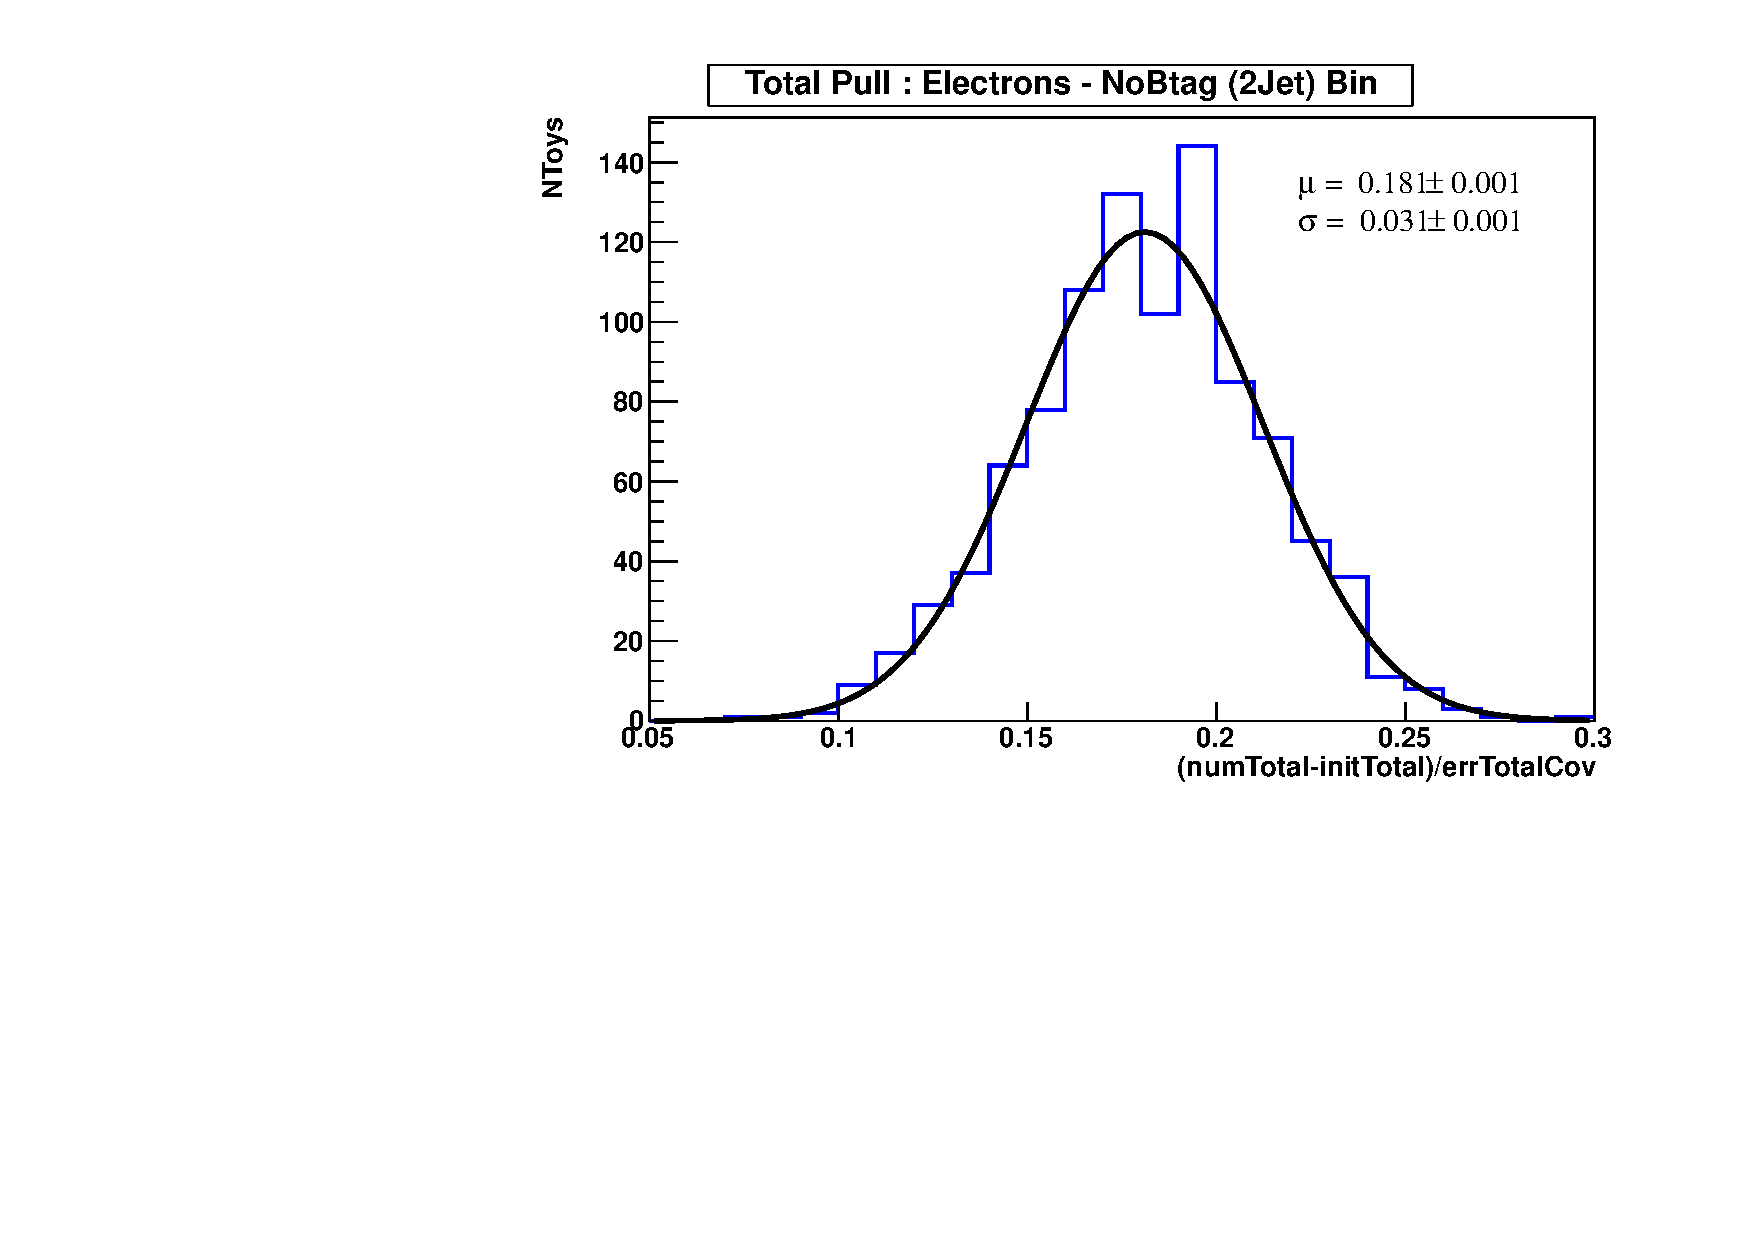
\includegraphics[width=0.48\textwidth]{figs/validation/TotalPull_Validation_el_NoBtag_2j.pdf}
\put(-0.80,0.0){(a)} 
\unitlength=0.33\linewidth
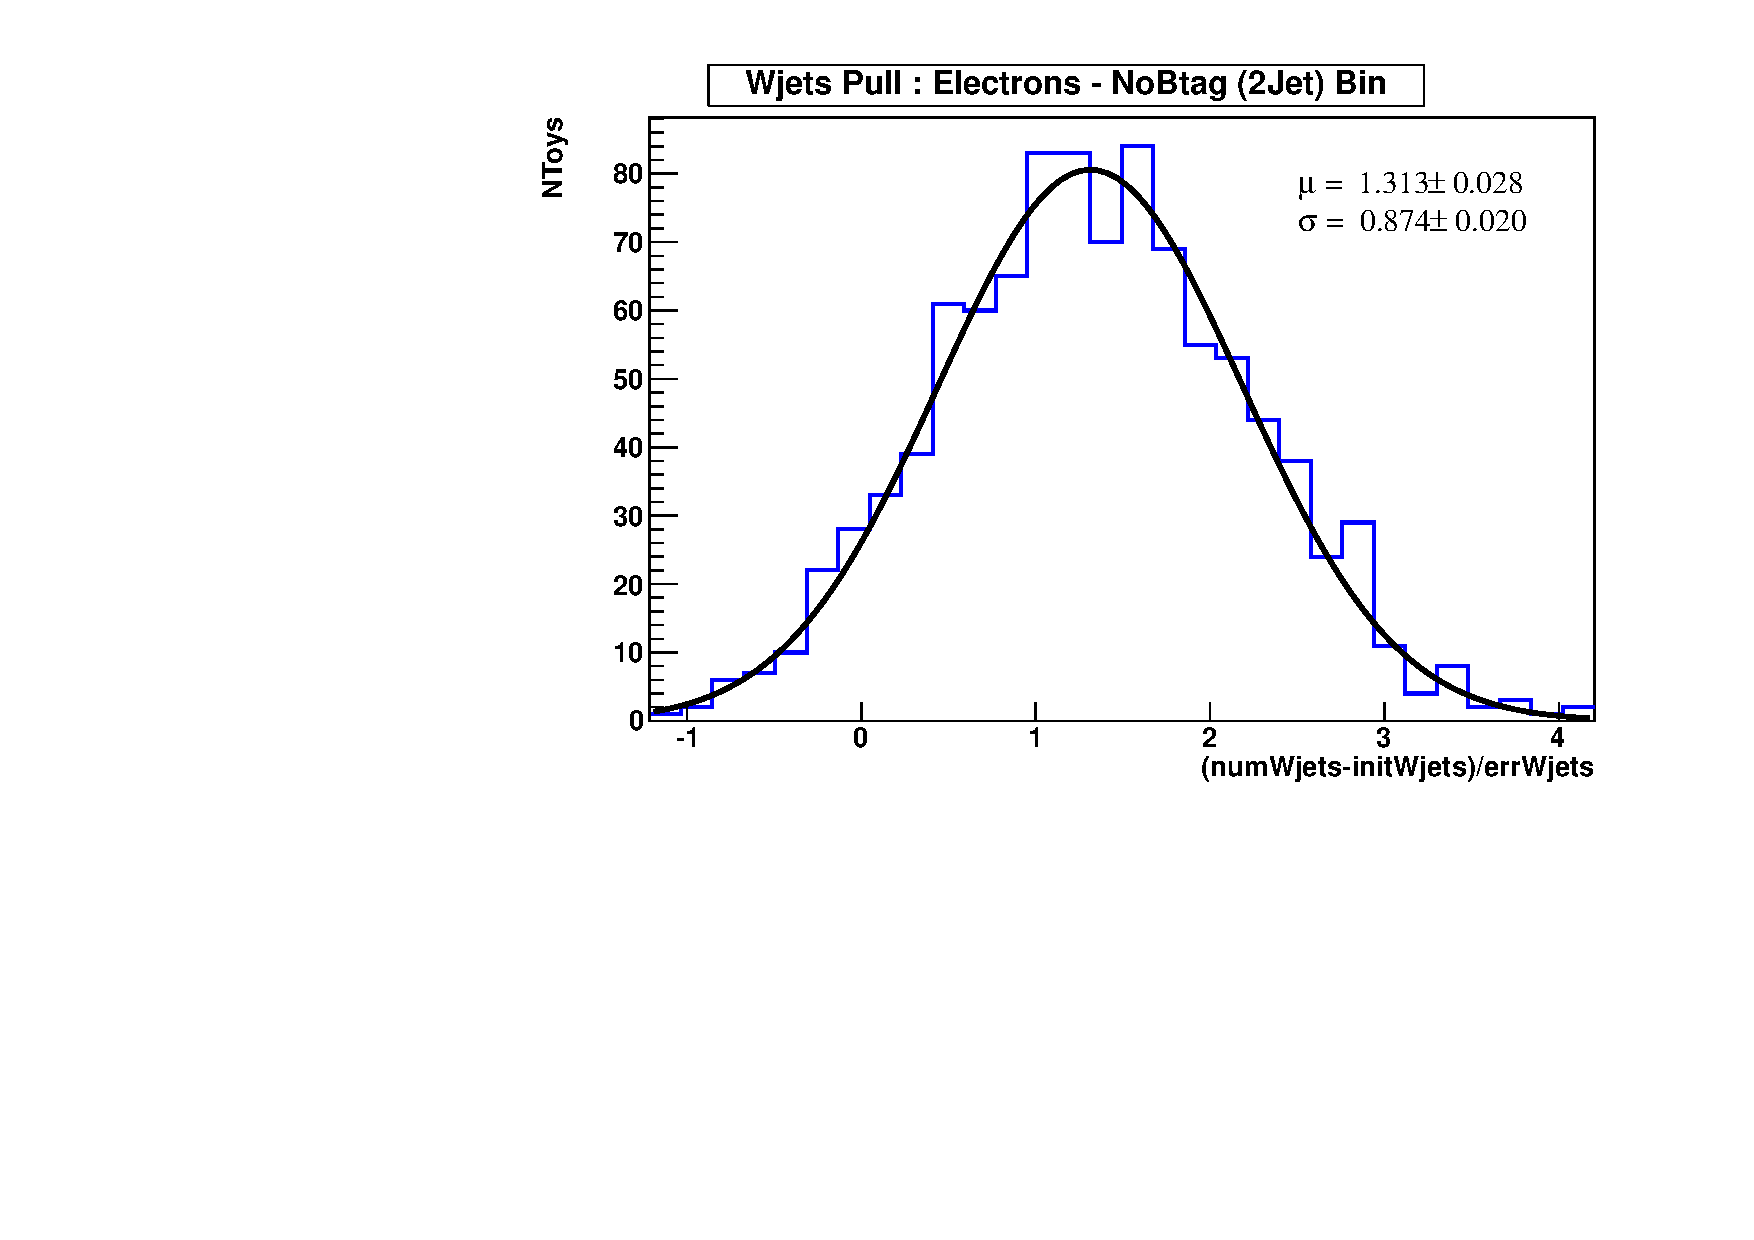
\includegraphics[width=0.48\textwidth]{figs/validation/WjetsPull_Validation_el_NoBtag_2j.pdf}
\put(-0.80,0.0){(b)}\\
\unitlength=0.33\linewidth
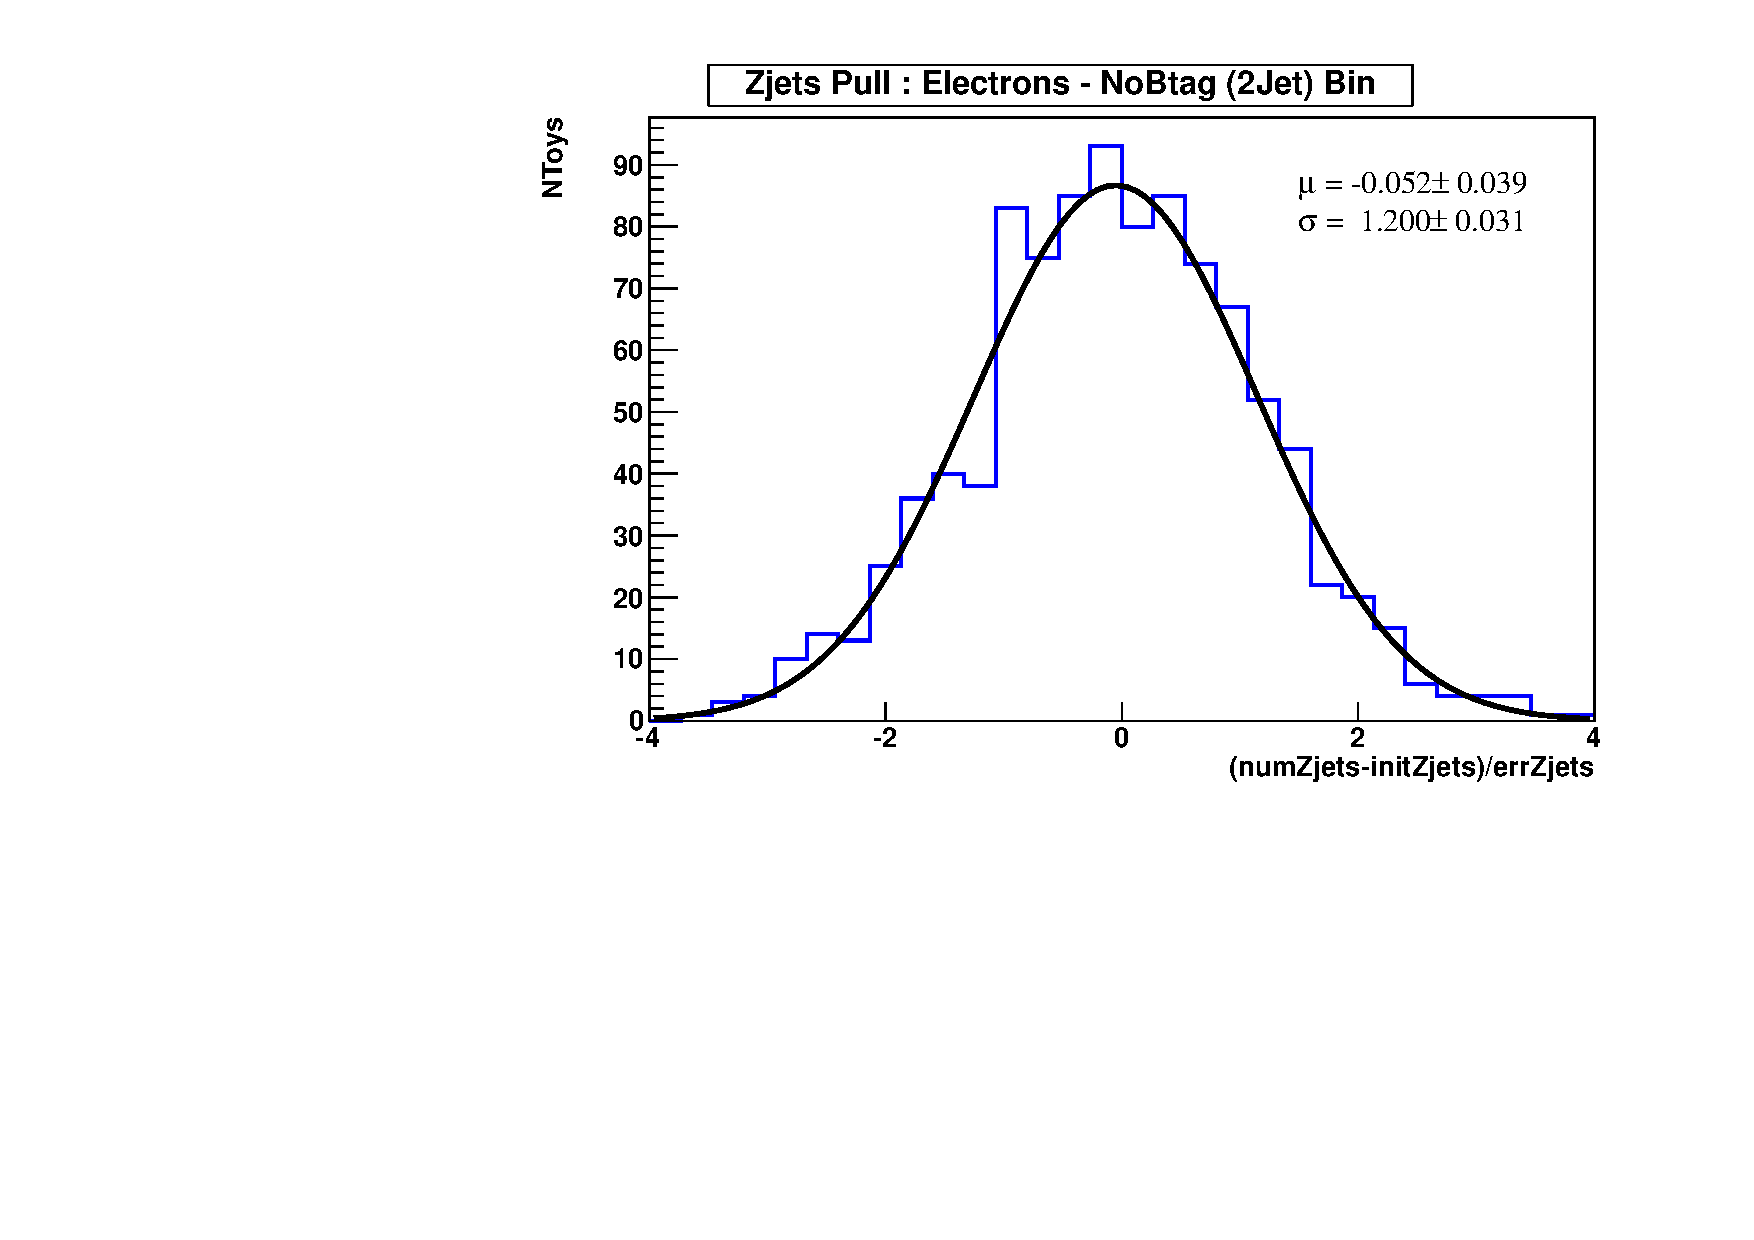
\includegraphics[width=0.48\textwidth]{figs/validation/ZjetsPull_Validation_el_NoBtag_2j.pdf}
\put(-0.80,0.0){(c)}
\unitlength=0.33\linewidth
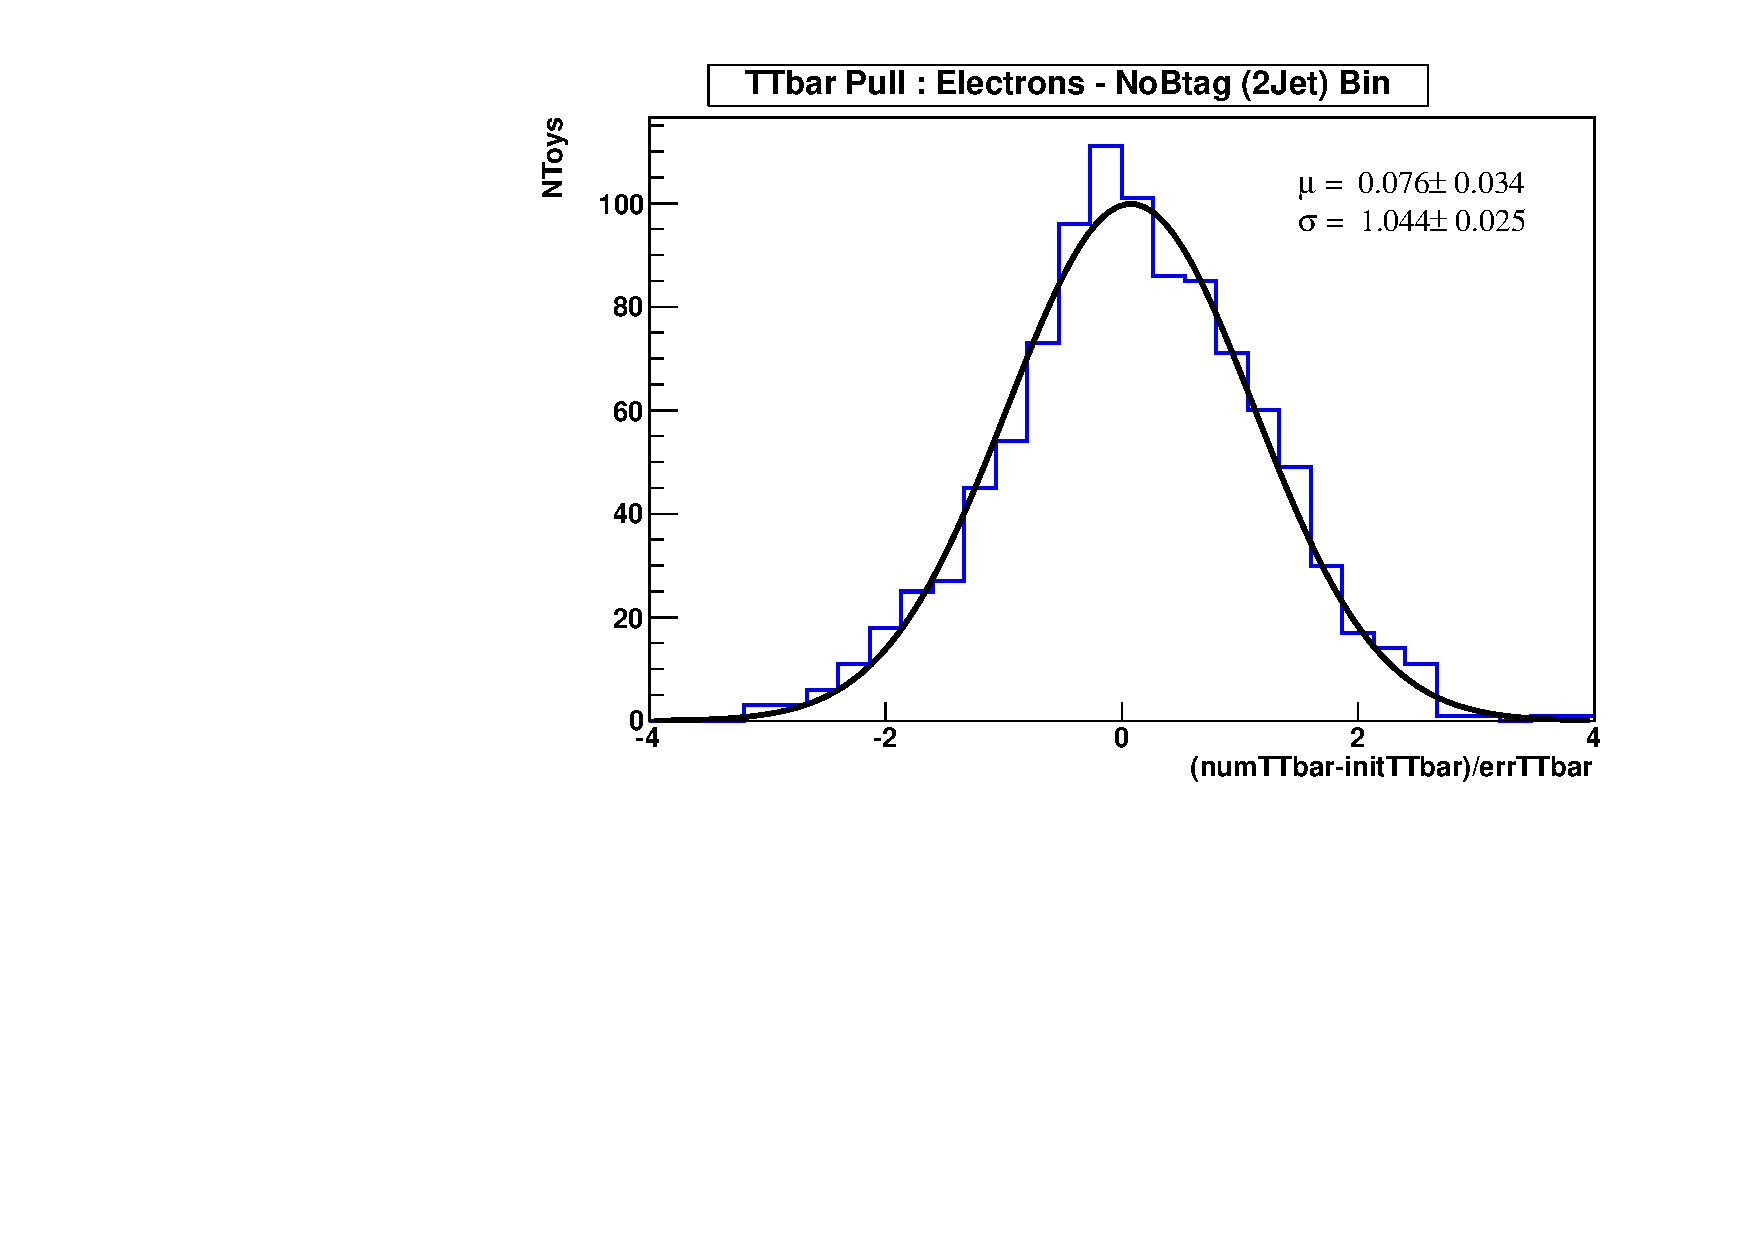
\includegraphics[width=0.48\textwidth]{figs/validation/TTbarPull_Validation_el_NoBtag_2j.pdf}
\put(-0.80,0.0){(d)}\\ 
\unitlength=0.33\linewidth
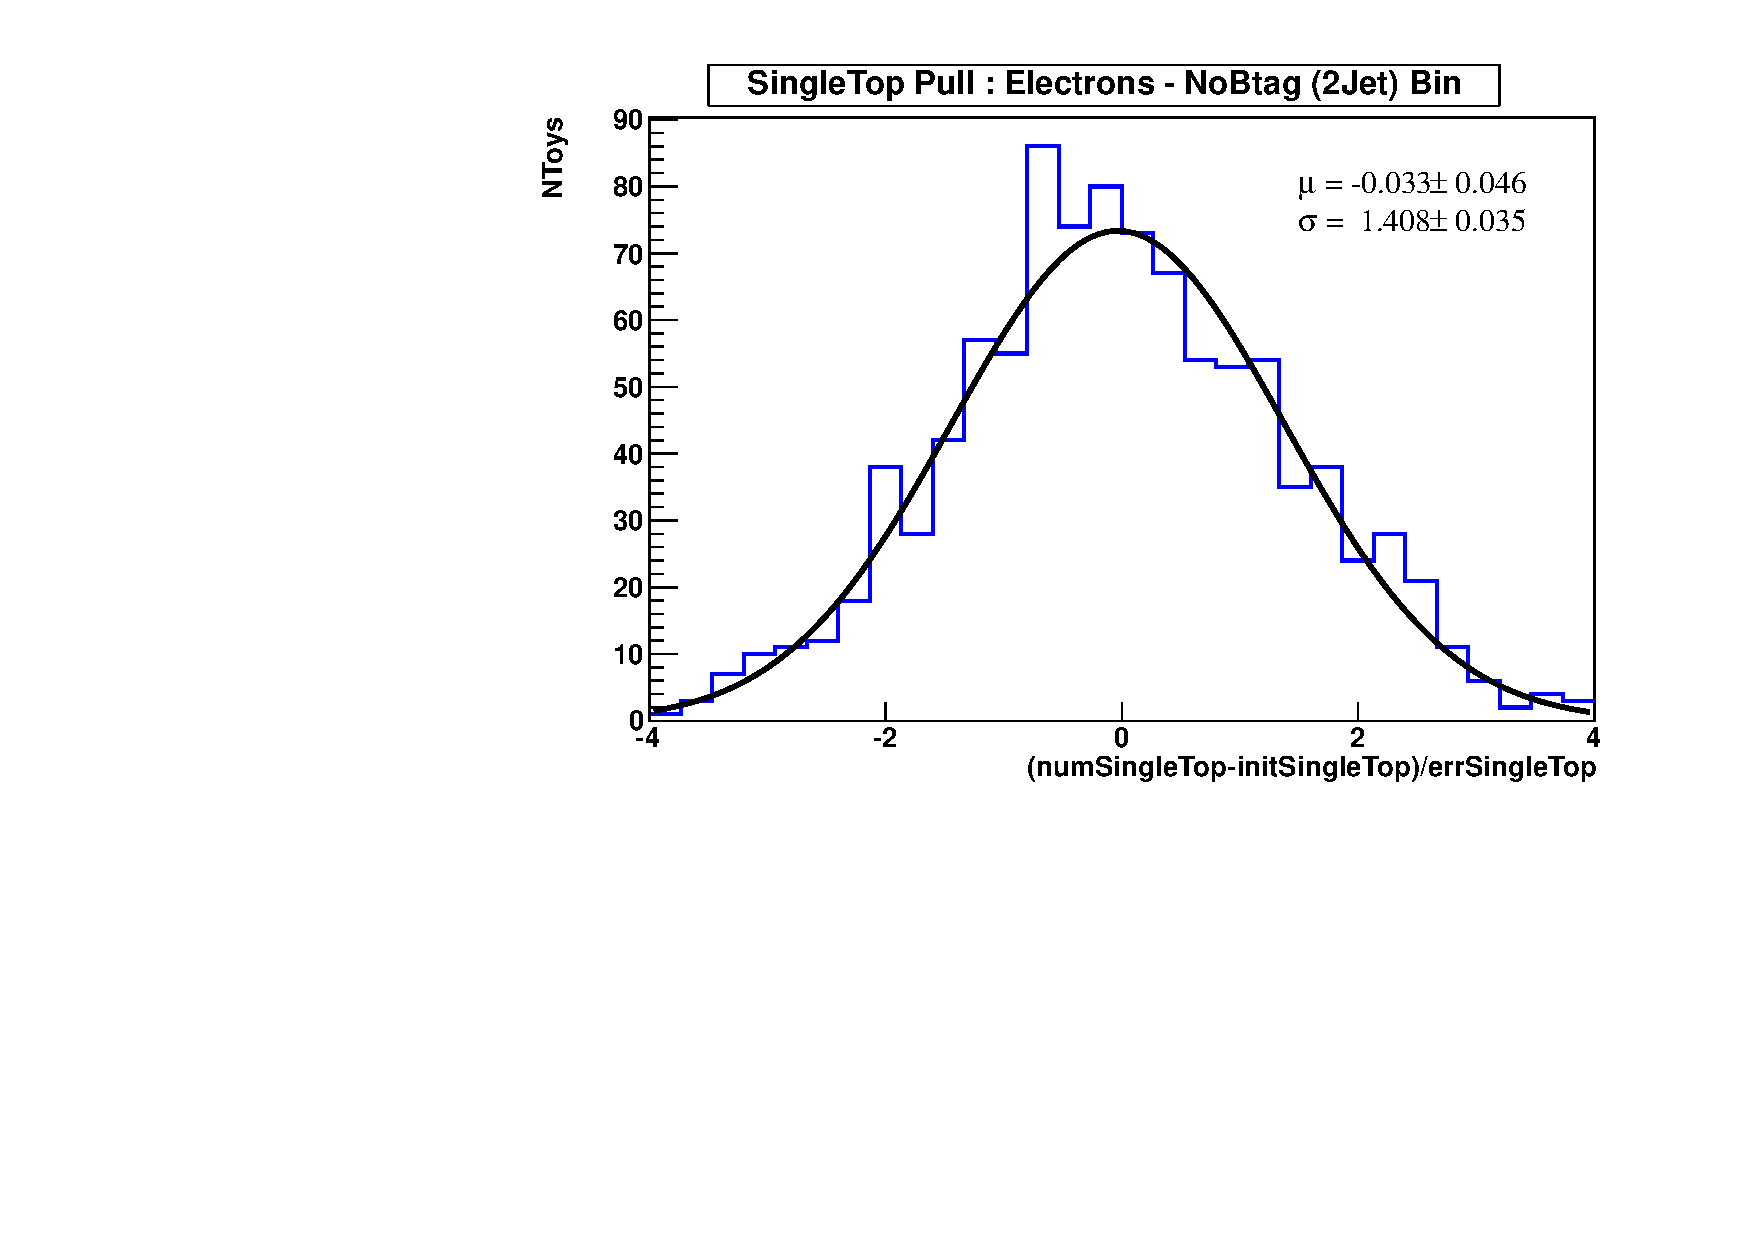
\includegraphics[width=0.48\textwidth]{figs/validation/SingleTopPull_Validation_el_NoBtag_2j.pdf}
\put(-0.80,0.0){(e)} 
\unitlength=0.33\linewidth
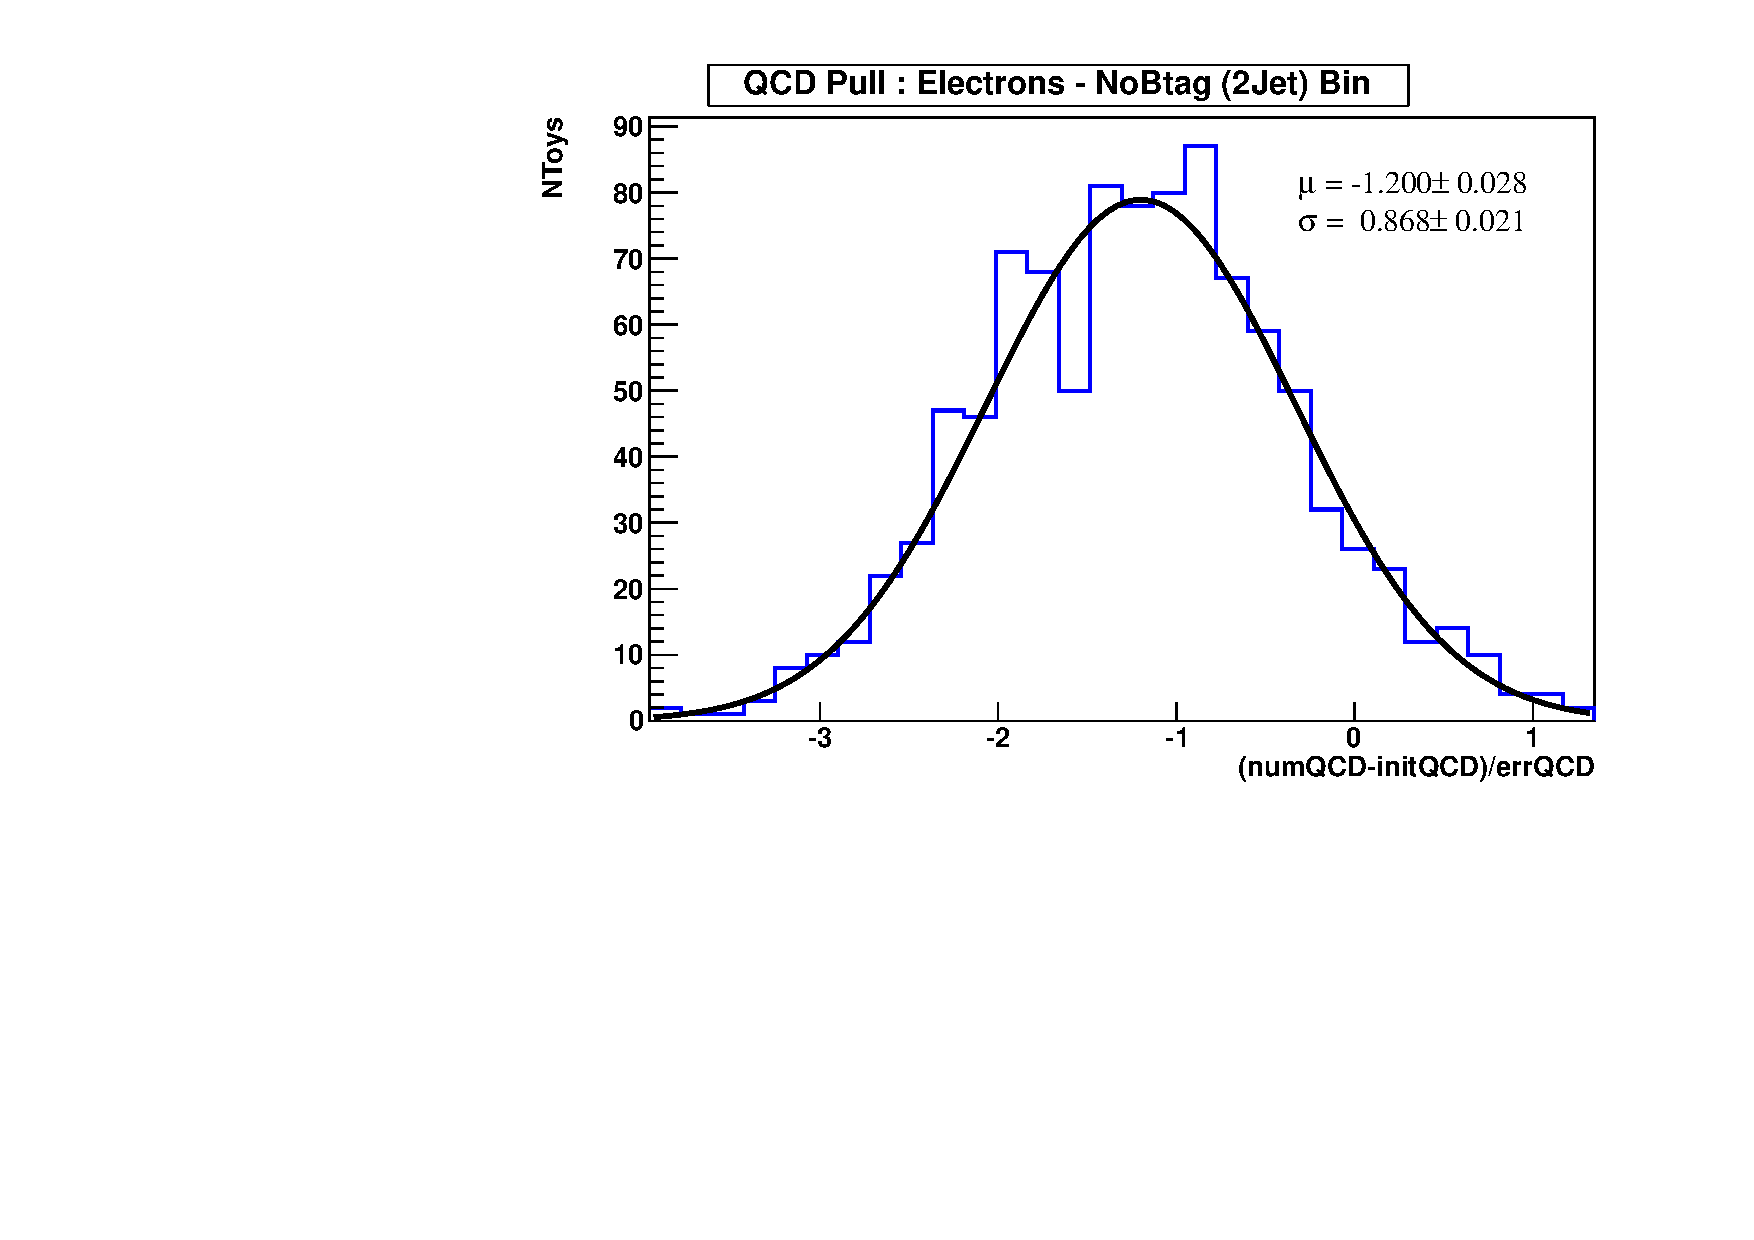
\includegraphics[width=0.48\textwidth]{figs/validation/QCDPull_Validation_el_NoBtag_2j.pdf}
\put(-0.80,0.0){(f)}\\
\unitlength=0.33\linewidth
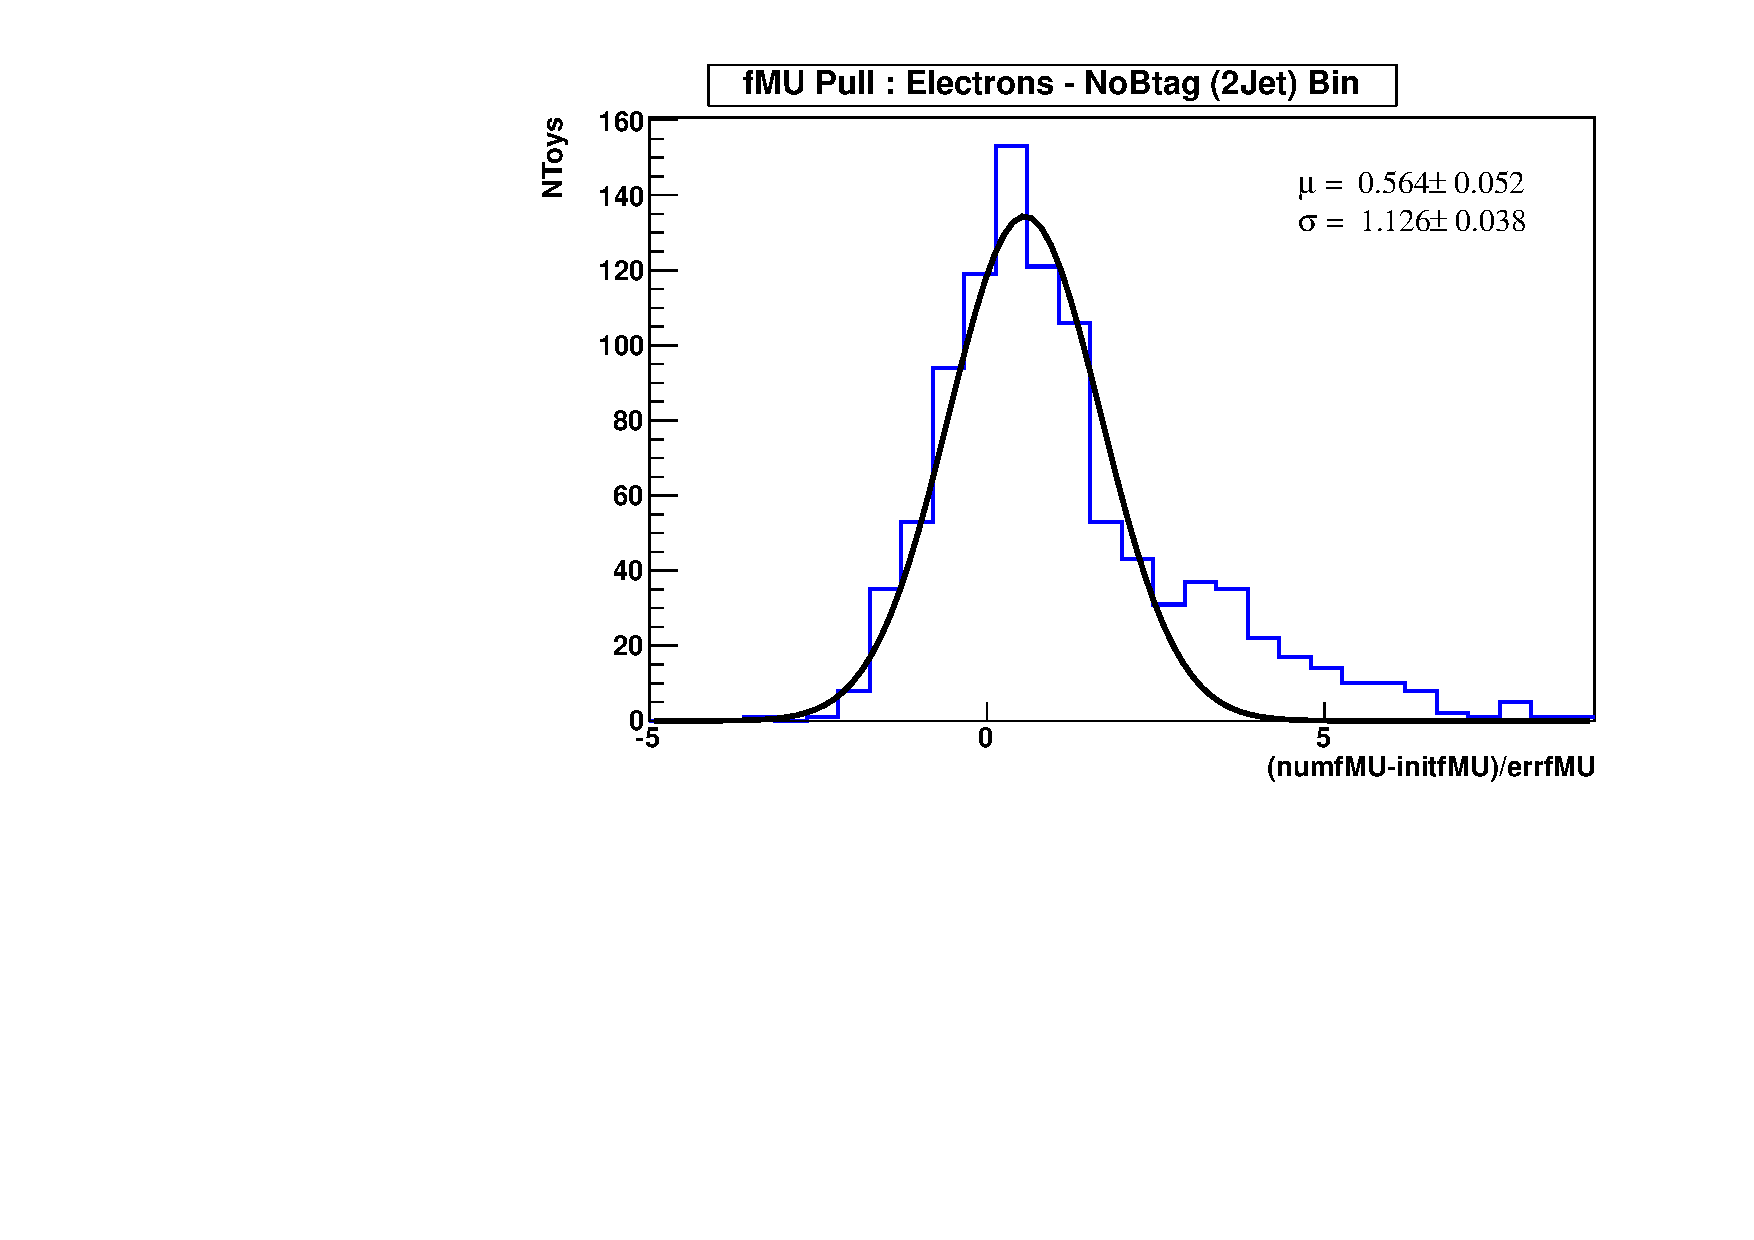
\includegraphics[width=0.48\textwidth]{figs/validation/fMUPull_Validation_el_NoBtag_2j.pdf}
\put(-0.80,0.0){(g)}
\unitlength=0.33\linewidth
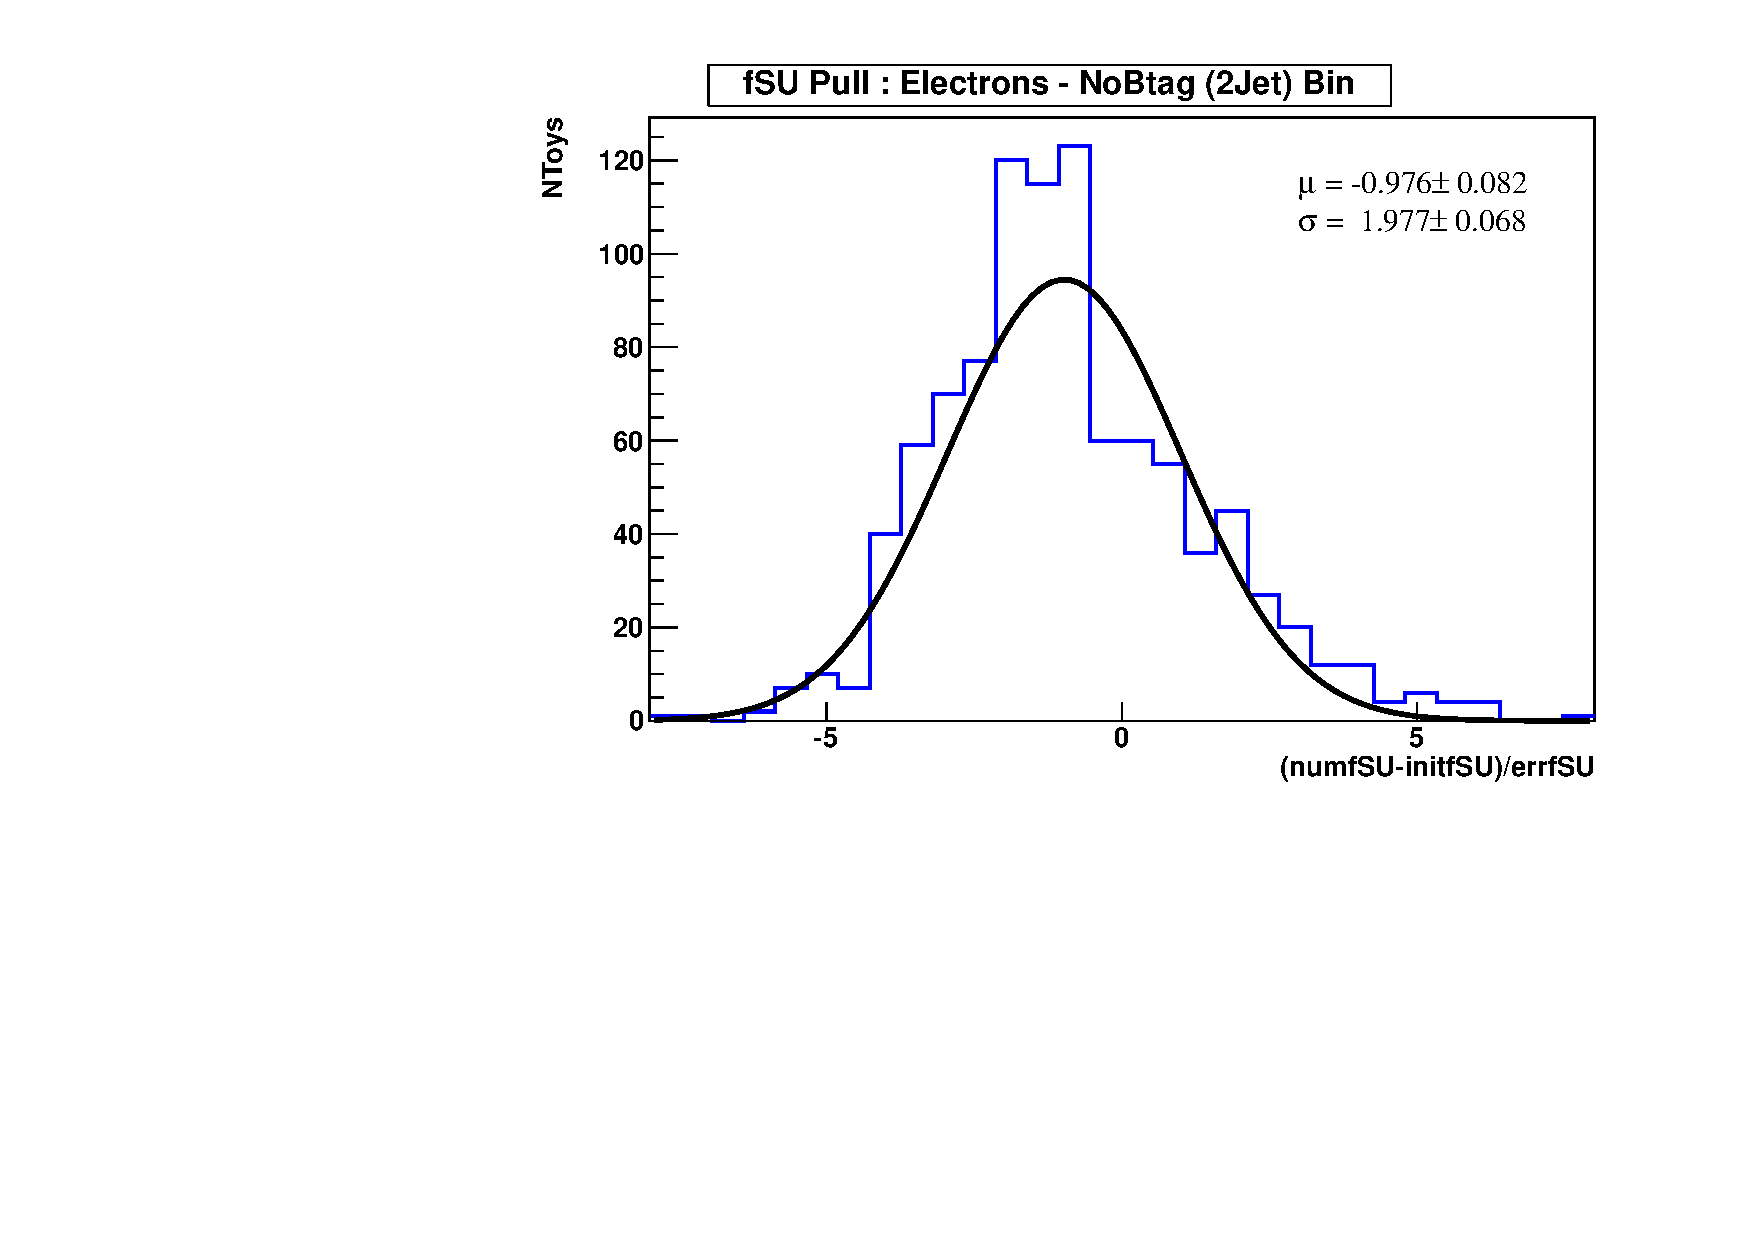
\includegraphics[width=0.48\textwidth]{figs/validation/fSUPull_Validation_el_NoBtag_2j.pdf}
\put(-0.80,0.0){(h)}
\caption{Fit validation in the  untagged (2-jet) bin of the electron channel, using 1000 Toy MC datasets. Pull=(Fitted-Given)/Error for: (a) Total, (b) W+jets, (c) Z+jets, (d) $t\bar{t}$, (e) SingleTop, (f) QCD, (g) Matching Up Fraction, (h) Scale Up Fraction.} 
\label{fig:Validation_Pulls_el_NoBTag_2j}}
\end{figure}
%%%%%%%
%%%%%%%%%%%%%%%%%%%%%%%%%%%%
%%%%%%%
\begin{figure}[h!] {\centering
\unitlength=0.33\linewidth
\includegraphics[width=0.48\textwidth]{figs/validation/TotalYield_Validation_fixedfMUfSU_mu_NoBtag_2j.pdf}
\put(-0.80,0.0){(a)}
\unitlength=0.33\linewidth
\includegraphics[width=0.48\textwidth]{figs/validation/DibosonYield_Validation_fixedfMUfSU_mu_NoBtag_2j.pdf}
\put(-0.80,0.0){(b)}\\ 
\unitlength=0.33\linewidth
\includegraphics[width=0.48\textwidth]{figs/validation/WjetsYield_Validation_fixedfMUfSU_mu_NoBtag_2j.pdf}
\put(-0.80,0.0){(c)} 
\unitlength=0.33\linewidth
\includegraphics[width=0.48\textwidth]{figs/validation/ZjetsYield_Validation_fixedfMUfSU_mu_NoBtag_2j.pdf}
\put(-0.80,0.0){(d)}\\
\unitlength=0.33\linewidth
\includegraphics[width=0.48\textwidth]{figs/validation/TTbarYield_Validation_fixedfMUfSU_mu_NoBtag_2j.pdf}
\put(-0.80,0.0){(e)} 
\unitlength=0.33\linewidth
\includegraphics[width=0.48\textwidth]{figs/validation/SingleTopYield_Validation_fixedfMUfSU_mu_NoBtag_2j.pdf}
\put(-0.80,0.0){(f)} 
\caption{Fit validation in the  untagged (2-jet) bin of the muon channel, using 1000 Toy MC datasets. The Matching and Scaling fractions are fixed to their expected values. Fitted-Given yields for: (a) Total, (b) Diboson, (c) W+jets, (d) Z+jets, (e) $t\bar{t}$, (f) SingleTop.} 
\label{fig:Validation_Yields_NoBTag_2j_fixedfMUfSU}}
\end{figure}
%%%%%%%
%%%%%%%
\begin{figure}[h!] {\centering
\unitlength=0.33\linewidth
\includegraphics[width=0.48\textwidth]{figs/validation/TotalPull_Validation_fixedfMUfSU_mu_NoBtag_2j.pdf}
\put(-0.80,0.0){(a)}
\unitlength=0.33\linewidth
\includegraphics[width=0.48\textwidth]{figs/validation/DibosonPull_Validation_fixedfMUfSU_mu_NoBtag_2j.pdf}
\put(-1.00,0.0){(b)}\\ 
\unitlength=0.33\linewidth
\includegraphics[width=0.48\textwidth]{figs/validation/WjetsPull_Validation_fixedfMUfSU_mu_NoBtag_2j.pdf}
\put(-0.80,0.0){(c)}
\unitlength=0.33\linewidth
\includegraphics[width=0.48\textwidth]{figs/validation/ZjetsPull_Validation_fixedfMUfSU_mu_NoBtag_2j.pdf}
\put(-0.80,0.0){(d)}\\
\unitlength=0.33\linewidth
\includegraphics[width=0.48\textwidth]{figs/validation/TTbarPull_Validation_fixedfMUfSU_mu_NoBtag_2j.pdf}
\put(-0.80,0.0){(e)} 
\unitlength=0.33\linewidth
\includegraphics[width=0.48\textwidth]{figs/validation/SingleTopPull_Validation_fixedfMUfSU_mu_NoBtag_2j.pdf}
\put(-1.00,0.0){(f)} 
\caption{Fit validation in the  untagged (2-jet) bin of the muon channel, using 1000 Toy MC datasets. The Matching and Scaling fractions are fixed to their expected values. Pull=(Fitted-Given)/Error for: (a) Total, (b) Diboson, (c) W+jets, (d) Z+jets, (e) $t\bar{t}$, (f) SingleTop.} 
\label{fig:Validation_Pulls_NoBTag_2j_fixedfMUfSU}}
\end{figure}
%%%%%%%
%%%%%%%
\begin{figure}[h!] {\centering
\unitlength=0.33\linewidth
\includegraphics[width=0.43\textwidth]{figs/validation/DibosonYield_Validation_muNoBtag2j_DbShiftm0p2.pdf}
\put(-0.70,0.0){(a)} 
\unitlength=0.33\linewidth
\includegraphics[width=0.43\textwidth]{figs/validation/DibosonPull_Validation_muNoBtag2j_DbShiftm0p2.pdf}
\put(-0.80,0.0){(b)}\\
\unitlength=0.33\linewidth
\includegraphics[width=0.43\textwidth]{figs/validation/DibosonYield_Validation_muNoBtag2j_DbShiftm0p1.pdf}
\put(-0.70,0.0){(c)}
\unitlength=0.33\linewidth
\includegraphics[width=0.43\textwidth]{figs/validation/DibosonPull_Validation_muNoBtag2j_DbShiftm0p1.pdf}
\put(-0.80,0.0){(d)}\\ 
\unitlength=0.33\linewidth
\includegraphics[width=0.43\textwidth]{figs/validation/DibosonYield_Validation_muNoBtag2j_DbShift0.pdf}
\put(-0.70,0.0){(e)} 
\unitlength=0.33\linewidth
\includegraphics[width=0.43\textwidth]{figs/validation/DibosonPull_Validation_muNoBtag2j_DbShift0.pdf}
\put(-0.80,0.0){(f)}\\
\unitlength=0.33\linewidth
\includegraphics[width=0.43\textwidth]{figs/validation/DibosonYield_Validation_muNoBtag2j_DbShiftp0p1.pdf}
\put(-0.70,0.0){(g)}
\unitlength=0.33\linewidth
\includegraphics[width=0.43\textwidth]{figs/validation/DibosonPull_Validation_muNoBtag2j_DbShiftp0p1.pdf}
\put(-0.80,0.0){(h)}\\
\unitlength=0.33\linewidth
\includegraphics[width=0.43\textwidth]{figs/validation/DibosonYield_Validation_muNoBtag2j_DbShiftp0p2.pdf}
\put(-0.70,0.0){(i)}
\unitlength=0.33\linewidth
\includegraphics[width=0.43\textwidth]{figs/validation/DibosonPull_Validation_muNoBtag2j_DbShiftp0p2.pdf}
\put(-0.80,0.0){(j)}
\caption{Fit validation in the untagged (2-jet) bin of the muon channel without fit-error smearing for default Diboson Yield $\times$ (a),(b) $0.8$; (c),(d) $0.9$; (e),(f) $1.0$; (g),(h) $1.1$;( i),(j) $1.2$. Diboson (a),(c),(e),(g),(i) Yields and (b),(d),(f),(h),(j) Pulls are displayed.} 
\label{fig:Validation_fixedCentralYields_Diboson_mu_NoBTag_2j}}
\end{figure}
%%%%%%%
%%%%%%%
\begin{figure}[h!] {\centering
\unitlength=0.33\linewidth
\includegraphics[width=0.96\textwidth]{figs/validation/DibosonYield_BiasScan_muNoBtag2j.pdf}
\caption{Diboson Yield Scan results in the untagged (2-jet) bin of the muon channel without fit-error smearing, using 1000 Toy MC datasets at each point. The distribution is fitted with a first order polynomial, which is statistically consistent with a constant function.} 
\label{fig:Validation_fixedCentralYields_BiasScan_mu_NoBTag_2j}}
\end{figure}
%%%%%%%
